%%!TEX encoding = UTF-8 Unicode

% Several lines in file have comments suggesting common packages for the
% typical thesis in informatics or electronics developed at UA
% uncomment/comment the lines as required for your work
% Before each optional line you will have a small comment

% According to UA rules, font size should range from 10 to 12pt.
\documentclass[11pt,a4paper,oneside,onecolumn]{memoir}

\listfiles
\fixpdflayout

\usepackage[utf8]{inputenc}

% Select Computer Modern Typewritter (For bold ttfamily in listings)
\usepackage{lmodern}
% OR... Bera Mono
%\usepackage[scaled]{beramono} % TTT Font
%\usepackage{anyfontsize} % As the name says...

\usepackage[T1]{fontenc}

% Enable for for Overleaf support
\usepackage{ifthen}
\def\useoverleaf{0}  % change to non-zero (for instance, 1) to enable it

\makeatletter
\newcommand{\makecoverfile}[0]{%
  \immediate\write18{latexmk -pdf cover.tex}%
}
\makeatother

% For PDF merging
\usepackage{pdfpages}

% Set DPI to 300
\pdfpxdimen=\dimexpr 1in/300\relax

% Allow the use of a larger number of packages
\usepackage{morewrites} 

% For English and Portuguese languages
% Portuguese will be the default.
% Uncomment \setlanguage below to change it
\usepackage[english,portuguese]{babel}

% Uncomment to use a custom date format
%\usepackage{datetime}
%\newdateformat{thesisdate}{\monthname[\THEMONTH] \THEYEAR} % Month Year

% Make pdf look better
\usepackage{microtype} 

% Uncomment to enable floats on facing pages
%\usepackage{dpfloat}

% Side by side figures
% Eg. Fig 1a, Fig 1b
\usepackage[hang,small,bf]{caption}
%\let\tion\undefined 
%\let\subfloat\undefined
\usepackage{subcaption}

%\RequirePackage{textcase}

% Dropped Caps
%\usepackage{lettrine}

% Configure Hyperlink color
% As a matter or style, you may use this to enable/disable color boxes on links
%\usepackage[breaklinks=true,colorlinks=false,linkcolor=blue]{hyperref}
% Or use the default values provided by the hyperref package
\usepackage{hyperref}

% Redefine section names according to your preference
%\def\sectionautorefname{Section}
%\def\chapterautorefname{Chapter}
%\def\figureautorefname{Figure}
%\def\listingautorefname{Listing}
%\def\tableautorefname{Table}

% Redefine code boxes
\ifthenelse{\equal{\useoverleaf}{0}}
{\usepackage[outputdir=build]{minted}}
{\usepackage{minted}}%

\addto\captionsportuguese{%
  \renewcommand\listingscaption{Código}
}
\fvset{fontsize=\footnotesize} % Make Code blocks smaller than text
\usepackage{csquotes}

% Add support for PDF Comments
\usepackage{comment}
\ifthenelse{\equal{\useoverleaf}{0}}
{\usepackage{pdfcomment}}{}
\usepackage{bookmark} % New Bookmarks

% For Multiple columns in Glossary
\usepackage{multicol}

% Add support for Math symbols
\usepackage{amsmath}
\usepackage{amssymb}

% Add support for graphics
\usepackage{graphicx}

% Add support for Colors
\usepackage{xcolor}

% Add support for the Euro symbol
\usepackage{eurosym}

% Add support for missingfigure and todo
\usepackage{todonotes}

% Setup bibliography with Biber using IEEE style for proper UTF-8 support
\usepackage[backend=biber, style=ieee, sorting=none, natbib=true, mincitenames=1, maxcitenames=2]{biblatex}
\bibliography{bib/references.bib}

% Use acronyms
\usepackage[printonlyused]{acronym} % For acronyms

% Indenting the first paragraph after section start
\usepackage{indentfirst}

% For fixing listoflistings with memoir
\usepackage{xparse} 

% Uncomment the next lines to enable chart support through pgf and tikz
% This may require you to install further packages in your Tex system
%\usepackage[version=0.96]{pgf}
%\usepackage{tikz}

% UML support
%\usepackage{pgf-umlsd}

% Trees, Arrows, Mindmaps and other popular objects
%\usetikzlibrary{arrows,shadows,trees,shapes,decorations,automata,backgrounds,petri,mindmap} % for pgf-umlsd

% Package to master SI units
\usepackage[detect-weight=true, binary-units=true]{siunitx}
% For Electric Circuits
%\sisetup{load-configurations = binary}

% Set Voltage direction accordingly
% Option : oldvoltagedirection,nooldvoltagedirection,RPvoltages,EFvoltages
% More information at: https://mirrors.ibiblio.org/CTAN/graphics/pgf/contrib/circuitikz/doc/circuitikzmanual.pdf
% By default this template is using the Old Voltage Direction
%\usepackage[oldvoltagedirection,american,cuteinductors,smartlabels]{circuitikz}
%\usetikzlibrary{calc}
%\ctikzset{bipoles/thickness=1}
%\ctikzset{bipoles/length=0.8cm}
%\ctikzset{bipoles/diode/height=.375}
%\ctikzset{bipoles/diode/width=.3}
%\ctikzset{tripoles/thyristor/height=.8}
%\ctikzset{tripoles/thyristor/width=1}
%\ctikzset{bipoles/vsourceam/height/.initial=.7}
%\ctikzset{bipoles/vsourceam/width/.initial=.7}
%\tikzstyle{every node}=[font=\small]
%\tikzstyle{every path}=[line width=0.8pt,line cap=round,line join=round]

% For inline TT text (e.g. code snippets)
\usepackage{verbatim}

% Frames around figures and allow force placement
\usepackage{float}

% Configure Float style
%\floatstyle{boxed}
%\restylefloat{table}
%\restylefloat{figure}
%\restylefloat{lstlisting}

% For test purposes you may use the lipsum package to create dummy text
\usepackage{lipsum} % REMOVE

%Keep floats inside section!
\usepackage[section]{placeins}
\let \oldsubsubsection \subsubsection
\renewcommand{\subsubsection}[2][]{
  \FloatBarrier
  \oldsubsubsection#1{#2}
}
\let \oldsubsection \subsection
\renewcommand{\subsection}[2][]{
  \FloatBarrier
  \oldsubsection#1{#2}
}
\let \oldsection \section
\renewcommand{\section}[2][]{
  \FloatBarrier
  \oldsection#1{#2}
}
\let \oldchapter \chapter
\renewcommand{\chapter}[2][]{
  \FloatBarrier
  \oldchapter#1{#2}
}



% Use the built-in division styling
\headstyles{memman}

% Include subsections in the TOC
\settocdepth{subsection}

% Numbering down to subsections as well
\setsecnumdepth{subsection}

% extra index for first lines
\makeindex[lines]

% Margins for University of Aveiro Thesis
\setlrmarginsandblock{3cm}{2.5cm}{*}
\setulmarginsandblock{3cm}{3cm}{*}
\checkandfixthelayout

% Or select your custom spacing to make any ajustment
%\addtolength{\parskip}{0.5\baselineskip}
\linespread{1.5}

\newcommand\mainmatterWithoutReset
{\edef\temppagenumber{\arabic{page}}%
  \mainmatter
  \setcounter{page}{\temppagenumber}%
}


%%%%%%%%%%%%%%%%%%%%%%%%%%%%%%%%%%%%%%%%%%%%%%%%%%
% Document begins here
%%%%%%%%%%%%%%%%%%%%%%%%%%%%%%%%%%%%%%%%%%%%%%%%%%

\begin{document}

% Fix the numbering scheme by having a ghost style for page numbering
\pagenumbering{Alph}

\ifthenelse{\equal{\useoverleaf}{0}}{}{\makecoverfile{}}%
\setcounter{page}{0}\includepdf[pages=-]{cover.pdf}

% Uncomment to enable English
%\selectlanguage{english}


% Front matter

%Custom Chapter style named `thesis`
\makechapterstyle{thesis}{% Based on ell
  \chapterstyle{default}
  \renewcommand*{\chapnumfont}{\normalfont\sffamily}
  \renewcommand*{\chaptitlefont}{\normalfont\Huge\sffamily}
  \settowidth{\chapindent}{\chapnumfont 111}
  \renewcommand*{\chapterheadstart}{\begingroup
    \vspace*{\beforechapskip}%
    \begin{adjustwidth}{}{-\chapindent}%
    \hrulefill
    \smash{\rule{0.4pt}{15mm}}
    \end{adjustwidth}\endgroup}
  \renewcommand*{\printchaptername}{}
  \renewcommand*{\chapternamenum}{}
  \renewcommand*{\printchapternum}{%
    \begin{adjustwidth}{}{-\chapindent}
    \hfill
    \raisebox{10mm}[0pt][0pt]{\fontsize{30}{25}\selectfont\chapnumfont \thechapter}%
                              \hspace*{1em}
    \end{adjustwidth}\vspace*{-3.0\onelineskip}}
  \renewcommand*{\printchaptertitle}[1]{%
    \vskip\onelineskip
    \raggedleft {\chaptitlefont ##1}\par\nobreak\vskip 4\onelineskip}}


% Select chapter style from existing or select custom
%\chapterstyle{thesis} % Others: dowding, demo2, dash, chappell, brotherton, bianchi, ger, madsen, tatcher, veelo,indexes)
% thesis can also be used as defined previously
% Check the memoir documentation for the available themes
% Default is veelo
\chapterstyle{veelo}
\makeoddfoot{plain}{}{\thepage}{} % Added by André Zúquete to fix a page numbering issue on the veelo chapter style

% Select Page style
\pagestyle{plain}

% If you feel adventurous you can also define all aspects of your theme
% Use either this input or the chapterstyle before
% % Rules
\newcommand{\thinRule}{\rule{\textwidth}{0.25pt}}

% Customize heading appearances
% Define styles
\newcommand{\partSize}{\Huge}
\newcommand{\partStyle}{\lsstyle\scshape}
\newcommand{\chapterSize}{\Huge}
\newcommand{\chapterStyle}{\lsstyle\scshape}
\newcommand{\chapterAfter}{}
\newcommand{\sectionSize}{\Large}
\newcommand{\sectionStyle}{\scshape\MakeTextLowercase}
\newcommand{\subsectionSize}{\large}
\newcommand{\subsectionStyle}{\scshape\MakeTextLowercase}
\newcommand{\subsubsectionSize}{\large}
\newcommand{\subsubsectionStyle}{\scshape\MakeTextLowercase}
\newlength{\partNumSizePt}
\setlength{\partNumSizePt}{60pt}
\newlength{\chapterNumSizePt}
\setlength{\chapterNumSizePt}{60pt}
\newcommand{\partNumSize}{%
  \fontsize{\partNumSizePt}{1.2\partNumSizePt}\selectfont%
}
\newcommand{\partNumStyle}{\partChapterNumColor}
\newcommand{\chapterNumSize}{%
  \fontsize{\chapterNumSizePt}{1.2\chapterNumSizePt}\selectfont%
}
\newcommand{\chapterNumStyle}{\partChapterNumColor}

% Customize parts
\renewcommand{\partnamefont}{\partSize\partStyle}
\renewcommand{\partnumfont}{\partNumSize\partNumStyle}
\renewcommand{\printpartname}{}
\renewcommand{\printparttitle}[1]{%
  \normalfont\normalcolor\partnamefont #1
}

% Customize chapters
\makeatletter
\setlength{\beforechapskip}{30pt}
\renewcommand*{\chapterheadstart}{\vspace*{\beforechapskip}}
\setlength{\afterchapskip}{3ex}
\setlength{\midchapskip}{3ex}
\renewcommand*{\chapnamefont}{%
  \Large\flushright\chapterStyle\partChapterNumColor%
}
\renewcommand*{\chapnumfont}{\chapterNumSize\chapterNumStyle}
\renewcommand*{\chaptitlefont}{%
  \normalfont\flushleft\normalcolor\chapterSize\chapterStyle%
}
\renewcommand*{\printchaptername}{%
  \chapnamefont\MakeTextLowercase{\@chapapp}%
}
\renewcommand*{\chapternamenum}{\quad}
\renewcommand*{\printchapternum}{%
%  \chapnumfont\textls[-75]{\classicstylenums{\thechapter}}%
 \chapnumfont\textls[-75]{\thechapter}%

}
\renewcommand*{\printchaptertitle}[1]{%
  \chaptitlefont #1
  \chapterAfter
}
\makeatother
% Customize sections and subsections
\setsecnumformat{\csname my#1\endcsname\quad}
\setsecheadstyle{\sectionSize\sectionStyle}
\newcommand{\mysection}{{\thesection}}
\setlength{\beforesecskip}{3em}


\setsubsecheadstyle{\subsectionSize\subsectionStyle}
\newcommand{\mysubsection}{{\normalfont\subsectionSize\thesubsection}}
\setlength{\beforesubsecskip}{3em}

\setsubsubsecheadstyle{\subsubsectionSize\subsubsectionStyle}
\newcommand{\mysubsubsection}{{\normalfont\subsubsectionSize\thesubsubsection}}
\setlength{\beforesubsubsecskip}{2em}

% Customize "Table of ..." appearance
% Customize headings
\newcommand{\renewPrintXTitle}[1]{%
  \renewcommand{#1}[1]{%
    \printchaptertitle{##1}%
  }%
}
\renewPrintXTitle{\printtoctitle}
\renewPrintXTitle{\printlottitle}
\renewPrintXTitle{\printloftitle}

% Customize ToC headings
\renewcommand{\cftpartfont}{\partChapterNumColor\partStyle}
\renewcommand{\cftchapterfont}{\chapterStyle}
\renewcommand{\cftsectionfont}{}
\renewcommand{\cftsubsectionfont}{}
\renewcommand{\cftfigurefont}{}
\renewcommand{\cfttablefont}{}
\newcommand{\cftlstlistingfont}{}

% Increase number width
\newlength{\cftNumWidthIncrease}
\setlength{\cftNumWidthIncrease}{0.25em}
\addtolength{\cftpartnumwidth}{\cftNumWidthIncrease}
\addtolength{\cftchapternumwidth}{\cftNumWidthIncrease}
\addtolength{\cftsectionindent}{\cftNumWidthIncrease}
\addtolength{\cftsubsectionindent}{\cftNumWidthIncrease}
% No leader dots
%\renewcommand*{\cftpartdotsep}{\cftnodots}
%\renewcommand*{\cftchapterdotsep}{\cftnodots}
%\renewcommand*{\cftsectiondotsep}{\cftnodots}
%\renewcommand*{\cftsubsectiondotsep}{\cftnodots}
%\renewcommand*{\cftfiguredotsep}{\cftnodots}
%\renewcommand*{\cfttabledotsep}{\cftnodots}
%\newcommand*{\cftlstlistingdotsep}{\cftnodots}
% Set page numbers immediately after entry text
\newcommand{\tocEntryPageSep}{\hspace{1em}}
\renewcommand{\cftpartleader}{\cftdotfill{\cftdotsep}}
%\renewcommand{\cftpartafterpnum}{\cftparfillskip}
%\renewcommand{\cftchapterleader}{\tocEntryPageSep}
\renewcommand{\cftchapterleader}{\cftdotfill{\cftdotsep}}
%\renewcommand{\cftchapterafterpnum}{\cftparfillskip}
\renewcommand{\cftsectionleader}{\cftdotfill{\cftdotsep}}
%\renewcommand{\cftsectionafterpnum}{\cftparfillskip}
\renewcommand{\cftsubsectionleader}{\cftdotfill{\cftdotsep}}
%\renewcommand{\cftsubsectionafterpnum}{\cftparfillskip}
\renewcommand{\cftfigureleader}{\cftdotfill{\cftdotsep}}
%\renewcommand{\cftfigureafterpnum}{\cftparfillskip}
\renewcommand{\cfttableleader}{\cftdotfill{\cftdotsep}}
%\renewcommand{\cfttableafterpnum}{\cftparfillskip}
\newcommand{\cftlstlistingleader}{\cftdotfill{\cftdotsep}}
%\newcommand{\cftlstlistingafterpnum}{\cftparfillskip}
% Customize page numbers
\newcommand{\tocPageStyle}{\tocPageColor}
\renewcommand{\cftpartpagefont}{\tocPageStyle}
\renewcommand{\cftchapterpagefont}{\tocPageStyle}
\renewcommand{\cftsectionpagefont}{\tocPageStyle}
\renewcommand{\cftsubsectionpagefont}{\tocPageStyle}
\renewcommand{\cftfigurepagefont}{\tocPageStyle}
\renewcommand{\cfttablepagefont}{\tocPageStyle}
\newcommand{\cftlstlistingpagefont}{\tocPageStyle}

% Abstract
% Remove indents around abstract text
\setlength{\absleftindent}{0pt}
\setlength{\absrightindent}{0pt}
% Change font size to conform with the rest of the document text
\renewcommand{\abstracttextfont}{\normalsize}

% Customize headers and footers including page numbers
\newcommand{\hfTextSize}{\footnotesize}
\newcommand{\headTextStyle}{\lsstyle\scshape\MakeTextLowercase}
\nouppercaseheads
\makeevenhead{headings}%
             {\hfTextSize\thepage}%
             {}%
             {\hfTextSize\headTextStyle\leftmark}
\makeevenhead{plain}%
             {\hfTextSize\thepage}%
             {}%
             {\hfTextSize\headTextStyle\leftmark}
\makeoddhead{headings}%
            {\hfTextSize\headTextStyle\rightmark}%
            {}%
            {\hfTextSize\thepage}
\makeoddhead{plain}%
            {\hfTextSize\headTextStyle\rightmark}%
            {}%
            {\hfTextSize\thepage}


% Customize captions
\newcommand{\captionSize}{\small}
\newcommand{\captionStyle}{\scshape}
\newcommand{\captionWidthRatio}{0.9}

\captionnamefont{\captionSize\captionStyle}
\captiontitlefont{\captionSize}
\captiondelim{ -- }
\captiontitlefinal{}
\changecaptionwidth
%\captionwidth{\captionWidthRatio\textwidth}

% Define colors
%\newcommand{\titleColor}{\color[rgb]{0.616, 0.0627, 0.176}}
\newcommand{\titleColor}{\color[rgb]{0,0,0}}

\newcommand{\partChapterNumColor}{\titleColor}
\newcommand{\dropCapColor}{\titleColor}
%\newcommand{\tocPageColor}{\color[rgb]{0.0980, 0.329, 0.651}}

\newcommand{\tocPageColor}{\color[rgb]{0, 0,0}}
\definecolor{shade0}{rgb}{1.0 , 1.0 , 1.0 }
\definecolor{shade1}{rgb}{0.9 , 0.9 , 0.9 }
\definecolor{shade2}{rgb}{0.8 , 0.8 , 0.8 }
\definecolor{shade3}{rgb}{0.65, 0.65, 0.65}
\definecolor{shade4}{rgb}{0.45, 0.45, 0.45}
\definecolor{shade5}{rgb}{0.0 , 0.0 , 0.0 }



%Exclude sub figures from List of Figures
%\captionsetup[subfloat]{list=no}

% Texts
\newenvironment{introduction}
{%
  \begin{minipage}{\textwidth}%
   \itshape%
}
{%
  \end{minipage}%
  \par\addvspace{2\baselineskip plus 0.2\baselineskip minus 0.2\baselineskip}%
}

\frontmatter

\tightlists
\midsloppy
\raggedbottom

\setcounter{tocdepth}{2} %subsections are added to the TOC
\setcounter{secnumdepth}{4} %subsubsections are numbered

% Initial document tables start here: TOC, LOF, LOT, Glossary
% Table of contents with slightly smaller font
{\small\tableofcontents}

% List of figures with slightly smaller font
\clearpage
{\small\listoffigures}

% List of tables with slightly smaller font
\clearpage
{\small\listoftables}

% List of code snippets

% Fix for Listings with memoir

\RenewDocumentCommand \chapter { s O{#3} m }{%
  \FloatBarrier
  \IfValueTF{#1}  % if optional star is seen
    {\oldchapter*{#2}}
    {\oldchapter#1{#2}}
}

%\renewcommand{\listingscaption}{Código}
%\renewcommand{\listoflistingscaption}{Lista de Excertos de Código}
%\clearpage
%{\small\listoflistings}
%\addcontentsline{toc}{chapter}{\listoflistingscaption}

% Reset Chapters
\renewcommand{\chapter}[2][]{
  \FloatBarrier
  \oldchapter#1{#2}
}

% Print Glossary
\clearpage
{\small\chapter{Glossary}

\footnotesize
\SingleSpacing

\begin{multicols}{2}
\begin{acronym}[AAAAAA]

	\acro{ev}[EV]{Eletric Vehicle}
	% \acro{CAGR}[CAGR]{Compound Annual Growth Rate}
	% \acro{ORM}[ORM]{Object-Relational Mapping}
	\acro{MVC}[MVC]{Model-View-Controller}
	\acro{UI}[UI]{User Interface}
	\acro{PWA}[PWA]{Progressive Web App}
	\acro{IEETA}[IEETA]{Institute of Electronics and Informatics Engineering of Aveiro}
	% \acro{RAD}[RAD]{Rapid Application Development}
	\acro{FURPS}[FURPS]{Functionality Usability Reliability Performance Supportability}
	\acro{CMMS}[CMMS]{Computerized Maintenance Management System}
	\acro{emel}[EMEL]{Empresa de Mobilidade e Estacionamento de Lisboa}
	\acro{SQL}[SQL]{Structured query language}
	\acro{HTML}[HTML]{Hypertext Markup Language}
	\acro{CSS}[CSS]{Cascading Style Sheets}
	\acro{JS}[JS]{JavaScript}
	\acro{aspnet}[ASP.NET]{Active Server Pages .NET}
	\acro{csharp}[C\#]{C Sharp}
	% \acro{UX}[UX]{User Experience}
	\acro{OS}[OS]{Operating System}
	\acro{PHP}[PHP]{Hypertext Preprocessor}
	\acro{mariadb}[MariaDB]{Maria Database, an open-source relational database management system}
	\acro{ai}[AI]{Artificial Intelligence}
	\acro{rdbms}[RDBMS]{Relational Database Management System}
	\acro{sms}[SMS]{Short Message Service}
	\acro{PBS}[PBS]{public bike share, a system that provides bicycles for shared use across multiple stations}
	\acro{servqual}[SERVQUAL]{Service Quality Model, a framework for measuring the gap between customer expectations and perceptions of service}
	\acro{likert}[Likert Scale]{A psychometric scale commonly used in questionnaires to measure attitudes or opinions, typically ranging from strongly disagree to strongly agree}
	\acro{kpi}[KPI]{Key Performance Indicator, a measurable value that demonstrates how effectively an organization achieves objectives}
	\acro{qa}[QA]{Quality Assurance, a process to ensure that products and services meet defined quality standards}
	\acro{pm}[PM]{Preventive Maintenance, a proactive approach that schedules regular maintenance to prevent equipment failures and reduce downtime}
	\acro{agile}[Agile]{A software development methodology emphasizing iterative development, collaboration, and flexibility}
	\acro{scrum}[Scrum]{An Agile framework for managing complex projects through iterative sprints and continuous feedback}
	\acro{hcd}[HCD]{Human-Centered Design, a design approach that prioritizes user needs and feedback during development}
	\acro{rest}[REST]{Representational State Transfer, an architectural style for designing networked APIs}
	\acro{api}[API]{Application Programming Interface}
	\acro{SUS}[SUS]{System Usability Scale}
	\acro{gps}[GPS]{Global Positioning System}
	\acro{URL}[URL]{Uniform Resource Locator}
	\acro{ef}[EF]{Entity Framework}
	\acro{csat}[Customer Satisfaction]{Customer Satisfaction, a key performance indicator that measures how satisfied customers are with a product or service}

\end{acronym}
\end{multicols} 

}

%%%%%%%%%%%%%%%%%%%%%%%%%%%%%%%%%%%%%%%%%%%%%%%%%%%%%%%
% Main document starts here
%%%%%%%%%%%%%%%%%%%%%%%%%%%%%%%%%%%%%%%%%%%%%%%%%%%%%%%

\mainmatter

% Line spacing: 1.5 pt 
\OnehalfSpacing

%%%%%%%%%%%%%%%%%%%%%%%%%%%%%%%%%%%%%%%%%%%%%%%%%%%%%%%
% Start of Thesis text 
%%%%%%%%%%%%%%%%%%%%%%%%%%%%%%%%%%%%%%%%%%%%%%%%%%%%%%%

% Uncomment to add further chapters
\chapter{Introduction}%
\label{chapter:introduction}

\begin{introduction}
% This chapter establishes the foundation for the dissertation by presenting the motivation behind the work, the main objectives to be achieved, and the problems that guided the development of the proposed solution. The rapid growth of vehicle-sharing services, combined with the increasing demand for sustainable transport, has intensified the need for efficient maintenance systems. However, many service providers still rely on outdated or manual approaches that can lead to inefficiencies, errors, and ultimately a loss of customer trust.

To address these challenges, this dissertation proposes the design and implementation of a \textbf{web-based platform} to support the daily operations of LightMobi's dealerships. The chapter begins by discussing the market context and the reasons why maintenance management is a critical concern. It then introduces the objectives of the system and highlights the problems that arise in current practices. Finally, it outlines the structure of the thesis.

\end{introduction} 


\section{Motivation}

The \textbf{vehicle-sharing} market has grown significantly since 2021 due to the global interest in sustainability and environmental issues. ~\cite{cohesionOpenData} ~\cite{bike_data_businessresearch}
The bike-sharing market, in particular, has gained popularity from governments worldwide, which are investing in cycling infrastructure such as cycling lanes, secure parking facilities, bicycle production and repair industries ~\cite{Clercq2023} ~\cite{Cerro2024} ~\cite{European_declararion_on_cycling} ~\cite{bike_data_businessresearch} ~\cite{cohesionOpenData}.
This attention to this sector raises the need for vehicle maintenance infrastructure that may be outdated and inefficient. ~\cite{MAS_MOTORS}
This low quality of service can lead to a significant decrease in the loyalty of the customers, which is the main source of income. ~\cite{Setting_the_after_sale_process}

The company \ac{EMEL}, responsible for the management of urban mobility in Lisbon, operates the public bike-sharing system GIRA. This service currently includes around 1,800 bicycles distributed across 159 stations, supporting an average of 7,405 trips per day ~\cite{Gira_Trips}. To ensure safety and reliability, bicycles undergo preventive maintenance either every 50 trips or every 14 days, depending on which threshold is reached first. On average, \ac{EMEL} performs about 70 maintenance operations per day ~\cite{Gira_Maintenance}. Given the scale of operations and the complexity of coordinating maintenance tasks across vehicles and stations, \ac{EMEL} requires an efficient system to organize and optimize this process, minimizing downtime while maximizing service availability.

This dissertation presents a software solution that facilitates and organizes the work processes at the dealerships of a vehicle sharing manufacturer as well as at \ac{EMEL}. 

The solution requirements will be gathered through direct communication with employees from both organizations, and its effectiveness will be validated with ordinary users.


\section{Objectives and problems}

The work at a workshop may be organized by manual input or with rudimentary applications. ~\cite{MAS_MOTORS} 
This may introduce accidental human errors, which in turn lead to break of promises or unsatisfaction from the customer. ~\cite{MAS_MOTORS} ~\cite{Setting_the_after_sale_process}
This type of approach may not be very prejudiced in a small business of 20 bicycles, but the continuous growth of the company requires a more modern method to handle the huge amount of work and achieve continuous success. ~\cite{MAS_MOTORS}

This dissertation will focus on the development of a web application that aims to facilitate and increase the work performance at a dealership. 

This dissertation presents a significant challenge related to the users who work at the dealerships and garages. 
These users may be already accustomed to their systems or their manual work's labor.  
The introduction of a new system may be a challenge to the users, so the system must be user-friendly, easy to use, and provide significant value in their work.

Another requirement is the integration with the fleet management platform of vehicle sharing, a project that has been in development for a few years with a team in \ac{IEETA} at the University of Aveiro.
It is a platform to manage the vehicle sharing system of an entity like hotels, city hall, etc.  

\section{Structure of the Thesis}


This dissertation is organized into six chapters, each addressing a specific stage of the research and development process:


\begin{itemize}
    \item Chapter 1 – \textbf{Introduction}: Presents the motivation for the work, the main objectives, and the challenges that the proposed solution aims to address.
    \item Chapter 2 – \textbf{Literature Review}: Discusses the theoretical foundations of the research, surveys existing solutions, and examines real-world scenarios relevant to maintenance management.
    \item Chapter 3 – \textbf{Requirements Analysis}: Defines the functional and non-functional requirements of the system, supported by detailed use cases that guide the design and implementation.
    \item Chapter 4 – \textbf{System Design and Implementation}: Describes the developed solution, including the database structure, the application's layout, and the main features implemented for each user role.
    % \item Chapter 5 – \textbf{Validation and Results}: Presents the evaluation process, including user testing with LightMobi's employee, external users, and the EMEL company, followed by an analysis of the results and identified limitations.
    \item Chapter 5 – \textbf{Validation and Results}: Presents the evaluation process, including user testing with external users followed by an analysis of the results.
    \item Chapter 6 – \textbf{Conclusion and Future Work}: Summarizes the main findings and identified limitations, and outlines possible directions for future development.
\end{itemize}

This structure ensures a logical flow from the problem definition to the validation of the solution, concluding with reflections and prospects for further research.


\chapter{Literature Review}%
\label{chapter:literatureReview}

\begin{introduction}
The purpose of this chapter is to establish the theoretical and practical foundation for the development of the proposed solution. It begins by examining the vehicle maintenance process, highlighting its relevance to service quality and customer satisfaction. 

Then it incorporates real-world insights gathered from EMEL, the company responsible for operating Lisbon's Gira bike-sharing system. 

Next, it introduces the multiple concepts relevant to the thesis.

And finally, the chapter reviews existing software solutions in the market analyzing their strengths, limitations, and relevance to this dissertation.
\end{introduction} 

To gather relevant information for this topic, I conducted a literature search using the Scopus and Google Scholar platforms. In Scopus, I applied the query “\textit{Vehicle AND Maintenance AND Dealerships}”, which initially returned 49 papers. After a preliminary review of titles and abstracts, 24 were identified as potentially relevant. However, a closer analysis revealed that only three were directly applicable to this dissertation. Many of the discarded papers treated dealerships primarily as sales units of larger companies, which lies outside the scope of this work. Others focused on narrow applications of machine learning, such as predictive maintenance. While valuable in their own right, these approaches did not align with the dissertation's emphasis on web applications and maintenance process management.

A complementary search on Google Scholar yielded three additional studies related to the electric vehicle market in China. Although these works provided useful insights into international contexts, they were excluded as the focus of this dissertation is on maintenance operations rather than market-specific trends.

Ultimately, three papers were selected for detailed analysis. Two of them examined the vehicle maintenance process and highlighted the importance of service quality in ensuring customer satisfaction. The third presented a practical software solution with a use case comparable to the objectives of this dissertation. Together, these studies helped to define the research context and identify key problems and solutions to address during the development phase.

\section{Theoretical Concepts}

\subsection{Vehicle Maintenance}

Delivering vehicle maintenance services involves numerous activities, each crucial for maintaining service quality and ensuring customer satisfaction. 
Any deviation from these activities can negatively impact quality, leading to client dissatisfaction and loyalty loss. ~\cite{Setting_the_after_sale_process}
The loyalty of the client is the main source of income for the company, so it is important to maintain the quality of the service. ~\cite{Setting_the_after_sale_process}
To fulfill this requirement to the fullest, one must supervise every stage of the process. ~\cite{Setting_the_after_sale_process}


\begin{figure}[h]
  \caption{Macro-level Flow of a vehicle maintenance or repair service. This figure was inspired by figure 6: After Sales process from ~\citet{Setting_the_after_sale_process}.}
  \centering
  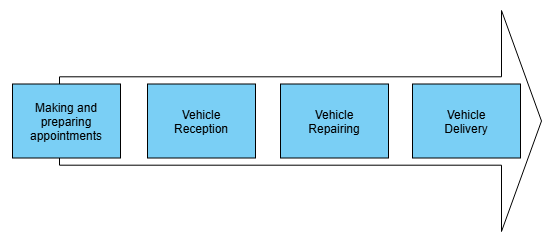
\includegraphics[width=0.50\textwidth]{figs/Vehicle_maintenace_macro}
  \label{fig:Vehicle_maintenace_macro}
\end{figure}

The general flow of vehicle maintenance is illustrated in the figure \ref{fig:Vehicle_maintenace_macro}. 
The first step of the process starts with a client interacting with the garage to schedule a vehicle maintenance or repair. 
After that, the client goes to the garage, where the receptionist receives the client and the vehicle.
Here, the mechanic will perform the maintenance of the vehicle and, when is done, the vehicle will be delivered to the client.

To ensure quality in the first step the receptionist must understand the fill capacity of the garage and the time to complete the job. 
With this information, the rececionist may accurately indicate the time to conclude the vehicle maintenance and get the client trust. ~\cite{Setting_the_after_sale_process}

In the second step, the receptionist and service advisor, when receiving the vehicle, must do a visual confirmation of the vehicle's condition. ~\cite{Setting_the_after_sale_process}
In this step, the receptionist explains to the client the services of the garage and they both agree with the services to be performed until a determined date. ~\cite{Setting_the_after_sale_process}

Following begins the third step and most important phase, the mechanic will perform the maintenance and repair of the vehicle. 
All of this process must be supervised by quality control to ensure that the job is done correctly. ~\cite{Setting_the_after_sale_process}
This includes the repair process, extra work, final tests, and service report. ~\cite{Setting_the_after_sale_process}
To accomplish that the use of a checklist is recommended to ensure precision and accuracy at each step. ~\cite{Setting_the_after_sale_process}

Finally, the last step is the delivery of the vehicle to the client. 
Here, the workshop manager must review the work done and the final price of the service to avoid extra payments from the client and incomplete payments to the workers. ~\cite{Setting_the_after_sale_process}

In this sense, the application of this dissertation will obey this flow.
For the receptionist and mechanic, the application will focus on reducing their mistake by giving accurate and illustrated information and making the work more effective.
And for the workshop manager to control the quality of the service with the assignment of tasks and authorization of purchases. 
Another user will be inserted into this flow, the warehouse operator, to manage the inventory of the dealership. 
The entire flow will be explained in Chapter III. 


\subsection{EMEL}


In June, I visited the company \ac{emel}, an entity responsible for operating and managing the public bike-sharing system Gira in Lisbon. This system comprises approximately 1,800 bicycles and 159 stations, supporting on average 7,405 trips per day, according to 2024 data ~\cite{Gira_Trips}. Each bicycle is scheduled for preventive maintenance either every 50 trips or every 14 days which results in an average of around 70 maintenance operations per day ~\cite{Gira_Maintenance}. This scale of demand requires a well-structured maintenance operation to ensure safety, reliability, and service availability.

To handle this demand, \ac{emel} follows a maintenance workflow that begins when a redistributor identifies a malfunction during routine operations and delivers the vehicle to the workshop. At this stage, the redistributor completes a paper form (Figures \ref{fig:emel_front} and \ref{fig:emel_back}), recording the detected faults and performing a simple diagnostic of electrical components such as the GPS unit and battery. If the vehicle fails these initial tests, it is set aside for a specialist to address before proceeding to standard maintenance. Otherwise, it enters a waiting list until a mechanic becomes available.

When a mechanic is free, the bicycle undergoes repair for both the reported issues and any additional problems detected during inspection. Upon completion, the mechanic records the parts used on the reverse side of the form. The bicycle is then forwarded to a quality control worker for validation. If defects are detected at this stage, the bicycle is returned to the same mechanic for correction before re-entering circulation. Although this process ensures that urgent faults are addressed, the high daily volume of bicycles forces \ac{emel} to prioritize speed over thoroughness, which can result in superficial inspections and undetected secondary issues.

These operational pressures also extend to inventory management. \ac{EMEL} collaborates with multiple suppliers under fixed contracts that specify delivery quantities and deadlines. This information is tracked manually through Excel spreadsheets, which are checked only at periodic intervals. This method provides limited insight into real-time consumption or future requirements. Without digital tools to integrate contract monitoring and inventory tracking, it becomes difficult to anticipate shortages or determine when new tenders should be initiated.

Introducing a digital system that integrates maintenance records with real-time inventory tracking would therefore enable \ac{emel} to optimize its resources, improve oversight, and maintain higher service quality despite the system's large operational scale.


\subsection{Computerized Maintenance Management System}

The software solution i will develop is a \ac{CMMS}.
A \ac{CMMS} is able to centralize and automate the management of maintenance operations, helping the dealership to manage the work tasks and the inventory, providing metrics to optimize the maintenance process.

It maintains a database with the information about the equipment, maintenance schedules, work orders, inventory, and personnel. 
It also document and reports all maintenance actions to facilitate the adherence to the regulatory standards ensuring the quality of the service. 
And analyzes the maintenance costs, downtime, efficiency, and other metrics to improve performence, optimization and reduce cost to the dealership.

The key benefits of the \ac{CMMS} are the improvement of the Preventive Maintenance, since it's easier to analyse the vehicle life and schedule a maintenance before the equipment failures occur; reduce costs, as the life of the vehicle is prolonged and the critical maintenace being avoided, this sofware provides a long-term cost saving; efficiency enhancement, by allowing the workers to focus on completing task instead of paperwork; and Regulatory Compliance, by keeping track and documenting the maintenance activities to comply by the organization standards. 

In conclusion, \ac{CMMS} provides a structured, data-driven approach to maintenance that enhances efficiency, reduces costs, ensures compliance, and ultimately supports the operational reliability of critical equipment and infrastructure.





\subsection{Service Quality}

Service quality is a critical factor in the success of vehicle maintenance services. One widely adopted framework for its evaluation is SERVQUAL, which provides a multidimensional approach for comparing consumers’ perceptions of service quality against their expectations. The model emphasizes five dimensions ~\cite{SERVQUAL_OLD}:


\begin{itemize}
   \item Tangibles – Physical facilities, equipment, and appearance of personnel.
   \item Reliability – Ability to consistently deliver services as promised.
   \item Responsiveness – Willingness to assist the customer and proactivity.
   \item Assurance – Demonstrate courtesy and knowledge and inspire trust and confidence.
   \item Empathy – Caring and treating customers as individuals.
  \end{itemize}

\begin{figure}[h]
  \caption{The 7-point Likert scale where the respondent may answer the question from strongly disagree to strongly agree. ~\cite{master_servqual_model}}
  \centering
  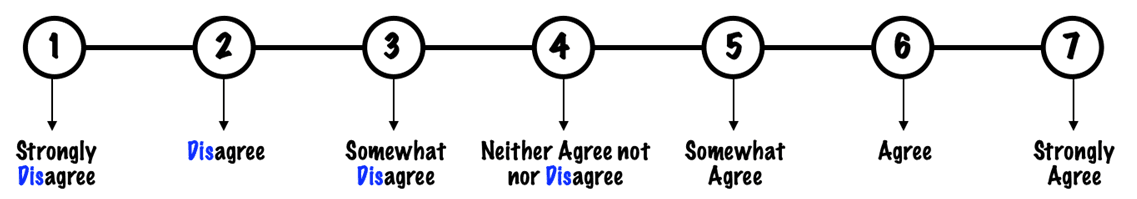
\includegraphics[width=\textwidth]{figs/likert_scale}
  \label{fig:likert_scale}
\end{figure}


To assess these dimensions, SERVQUAL relies on a questionnaire consisting of 22 items, divided across the five categories. Each item requires two ratings: one for the expectation of the service and another for the perception of the service received. The responses are given on a 7-point Likert scale, ranging from strongly disagree to strongly agree, as illustrated in Figure~\ref{fig:likert_scale} ~\cite{Measuring_After_sales_Service_Quality}. The quality gap is determined by the difference between the perception and expectation scores ~\cite{servqual_blog_da_qualidade} ~\cite{Measuring_After_sales_Service_Quality} ~\cite{SERVQUAL_OLD}.

An illustrative application of the SERVQUAL model can be found in the study by ~\citet{Measuring_After_sales_Service_Quality}, which assessed service quality at a CMV SA dealership in South Africa. The authors collected data through semi-structured questionnaires and interviews with customers, managers, and staff. The results, presented in Figure~\ref{fig:SERVQUAL_results}, revealed negative scores across all five dimensions, with an overall average gap of -0.10. These findings highlight that the services provided by the dealership consistently fell short of customer expectations. Among the main suggestions from customers were the expansion of workshops to reduce travel inconvenience and improving the availability of parts, which were often delayed due to international supply chains. The study underscores the importance of continuous service quality monitoring and recommends that dealerships regularly apply the SERVQUAL framework to identify and address performance gaps.

Building on this insight, this dissertation proposes the development of a client-facing application that enables users to evaluate the quality of service received, provide feedback, and make recommendations. This approach follows the SERVQUAL model and aims to strengthen customer trust and satisfaction.
\section{Existing solution}

\subsection{Fiix}
Fiix is a cloud-based \ac{CMMS} that allow organizations to manage their maintenance operations. 
It's main strengths lies on its advanced preventive maintenance scheduling, Comprehensive Work Order and Asset Management and AI-Powered Analytics and Reporting.

Despite the advantages of this software, Fiix has a high learning curve due to it's complexity and not intuitive old-fashion design interface. 
Also Fiix repordly lacks a built-in interal messaging system for crew communication. Most information sharing relies on notes and files attached to work orders, which may not be ideal for real-time collaboration.

With this effects in mind, i will aim in this software development to achieve a simple and user friendly solution where the users can intuitively interact with it by focusing on the key functional feature and easy navigation.

\subsection{Service Management for MAS Motors LLC}
MAS Motors LLC is a Toyota dealership in Libya that provides vehicle maintenance services. The company traditionally relied on manual processes, supported only by basic applications and paper-based documentation. While this approach was manageable at smaller scales, the expansion of the business exposed its inefficiencies and highlighted the need for a more modern solution ~\cite{MAS_MOTORS}. To address this challenge, ~\citet{MAS_MOTORS} developed a web application designed to streamline operations and enhance overall performance at the dealership.

The system was built to support multiple user groups—including service advisers, technicians, and customers—through a centralized platform that manages tasks such as job card handling, inventory updates, and customer service. The application was implemented using Laravel, a PHP web framework, together with MariaDB, an open-source relational database management system.

Evaluation results of the system were generally positive. A survey conducted with employees and customers assessed the solution using the \ac{FURPS} model, yielding scores of 4.27 for functionality, 4.30 for usability, 4.27 for reliability, 4.46 for performance, and 3.36 for supportability. While supportability received the lowest score—mainly due to limited configuration options ~\cite{MAS_MOTORS}—the system overall demonstrated clear improvements in service efficiency and customer satisfaction. Employees also provided valuable recommendations for future enhancements, including SMS-based service reminders, integration with social media platforms, and broader customer configuration options.

Building on these insights, my dissertation incorporates an email notification service, already used in the Lightmobie bike-sharing system, to handle alerts, user validation, and service-related notifications. This addition addresses part of the communication gap identified by MAS Motors employees while leveraging existing infrastructure within the Lightmobie ecosystem.

\subsection{Architecture Comparison}
  
The application will be developed using the ASP.NET Core MVC framework. This choice is motivated by several advantages over Laravel, the framework adopted in the solution proposed by ~\citet{MAS_MOTORS}. A detailed comparison between the two frameworks is presented in Table \ref{table:architetcture_comparison}.

One of the key advantages of ASP.NET Core MVC is its seamless integration with Microsoft SQL databases through the Entity Framework package, which greatly simplifies database interactions. While Laravel also supports relational database integration, ASP.NET Core MVC is generally more suitable for Microsoft environments ~\cite{asp_net_vs_laravel}.

In terms of performance, ASP.NET Core benefits from being based on C\#, a compiled language, whereas Laravel is built on PHP, an interpreted language. This distinction gives ASP.NET Core a performance edge, especially in applications that require scalability and responsiveness.

Security is another critical factor. Although Laravel provides features such as hashing and secure input validation, it requires deeper PHP expertise and continuous monitoring for vulnerabilities. ASP.NET Core, on the other hand, integrates more advanced security mechanisms out of the box, including role-based authentication and login management through the Identity Framework. These abstractions reduce the burden on the developer, allowing greater focus on application functionality ~\cite{asp_net_vs_laravel}.

\begin{table}[]
\begin{tabular}{| m{5em} | m{15em} | m{15em} |}
\hline
Parameter & Laravel & ASP.NET Core MVC \\
\hline
Language & PHP & C\# \\
\hline
Performance & Lower performance due to being an interpreted language & Higher performance due to being a compiled language \\
\hline 
Security & Provides features such as hashing and input validation, but requires strong PHP knowledge and manual management & Offers advanced built-in security tools, including role-based authentication and Identity Framework support \\
\hline
Integration with SQL & Supports various relational databases & Recommended for Microsoft environments due to strong integration packages \\
\hline
\end{tabular}
\caption{Comparison between Laravel and ASP.NET Core MVC frameworks for integration into the Lightmobie platform.}
\label{table:architetcture_comparison}
\end{table}
 
Another strong motivation for adopting ASP.NET Core MVC is its compatibility with Lightmobie's Fleet Management System, which follows the same architectural approach. This ensures easier integration, particularly for functionalities such as authentication and role assignment, which are already implemented and can be reused. While this choice may introduce some additional complexity, my prior involvement in developing the Fleet Management System provides familiarity with its features, thereby reducing the learning curve and facilitating a smoother integration process.
  

\section{Conclusion}

In this chapter i explained the theoretical concepts of the vehicle maintenance process in the literature and in the real case example EMEL in lisbon, and The SERVQUAL method to evaluate the quality of the service of a organization.
I also describe the existing solutions in the market, namely Fiix, and the results of MAS Motors LLC's application.
This solutions lack a intuitive interface and a notification service, so in this dissertation i will focus on accomplish that.


\chapter{Methodology}%
\label{chapter:methodology}

\begin{introduction}
In this chapter, i will present the non functional requirements of the applications, as well as the use cases of the user that will interact with them. 
\end{introduction} 




\section{Applications Requirements} 


To identify the requirements of the application, i used the FURPS model. 
The non functional requirements are listed below:

\begin{itemize}
  \item Scalability – The system should be able to handle 500 users simultaneously without degradading the performance.
  \item Reliability – The system should have a high availability of 99\% and the system also should not take longer then 4 hours to recover from a failure.
  \item Performance – The system should not take longer then 2 seconds to respond.
  \item Usability – The train of a new user should not take longer then 8 hours.
  \item Supportability – The system should be suported on the web browsers Chrome, Firefox, Microsoft Edge and Safari.
\end{itemize}

For the functional requirements of the applications, i developed a set of use cases for each user.
The structure of the dealership application was based on the work of the author ~\citet{Setting_the_after_sale_process} and is separated into 4 key user roles: receptionist, mechanic, warehouse operator and administrator.

The receptionist will be responsable to interact with the client, this includes the vehicle check-in and check-out and user comunication in the case of changes in the Initial stablished price and vehicle actions. 
The Use cases of the receptionist are:

\begin{itemize}
    \item Use Case 1.1 – Vehicle Reception
    \begin{itemize}
      \item Scenario – Client arrives at the dealership with a vehicle to be repaired.
      \item Objective – Create a new maintenance request in the system.
      \item System – The receptionist insert in the a form all the information about the initial maintenance request from the client and vehicle and creates a new maintenance request with the date and budget agreed with the client 
    \end{itemize}
    \item Use Case 1.2 – Vehicle Delivery 
    \begin{itemize}
      \item Scenario – The Receptionist delivered the vehicle to the Client.
      \item Objective – Complete the vehicle maintenance process.
      \item System – Sends a report in a pdf format to the client with the information of the maintenance request and alters the maintenance request status in the system to concluded. 
    \end{itemize}
    \item Use Case 1.3 – Collect information about a maintenance request
    \begin{itemize}
      \item Scenario – A Client call the dealership to ask about the maintenance of his vehicle.
      \item Objective – Visualize the maintenance information.
      \item System –  The Receptionist searches a list of maintenance requests by vehicle/customer name/maintenance ID and, by clicking on the element details button, he can view the maintenance details.
    \end{itemize}
    \item Use Case 1.4 – Asking for customer permission
    \begin{itemize}
      \item Scenario – O problem in a vehicle maintenance has occurred and the Initial agreement with client may be broken.
      \item Objective – Inform the client of the problem and achieve an agreement.
      \item System – The Receptionist receives an alert that there has been a change in the initial maintenance budget for a vehicle and/or a change in the maintenance completion deadline, so he needs to contact the customer to inform him. Depending on customer feedback, the receptionist accepts the request, declines the request or terminates the maintenance.
    \end{itemize}
  \end{itemize}  
  \hfill \break


  The mechanic will be responsable to do the maintenance in the vehicle, like oil change, tire change, trade vehicle parts, etc. 
  It will previously evaluate the vehicle, to assure the Initial evaluation of the receptionist is not lacking, and after the maintenance is done, it will write a report of the operations done. 
  The Mechanic Use cases are:

  \begin{itemize}
    \item Use Case 2.1 – View to-do list
    \begin{itemize}
      \item Scenario – The mechanic arrives at dealership and wants to see what tasks he has to do today.
      \item Objective – See the day's work organization.
      \item System – The mechanic watches a list of tasks that were assign from the administrator, as soon as he enters the system. Each task is accompany by a description, a priority, the vehicle identification, a set of actions to be performed and comments from other users. 
    \end{itemize}
    \item Use Case 2.2 – Carry out a vehicle analysis 
    \begin{itemize}
      \item Scenario – A new vehicle needs to be analyzed.
      \item Objective – Confirm the Initial analysis of the receptionist and search for additional problems.
      \item System – The mechanic enters the problems he finds in the vehicle into the system. 
    \end{itemize}
    \item Use Case 2.3 – Prepare a list of necessary parts
    \begin{itemize}
      \item Scenario – After vehicle analysis.
      \item Objective – Elaborate a request of vehicle parts for the warehouse.
      \item System – The mechanic selects the parts of the vehicle that need to be replaced and sends a request with the new parts to the warehouse.
    \end{itemize}
    \item Use Case 2.4 – Collect the requested parts in the Warehouse
    \begin{itemize}
      \item Scenario – The mechanic goes to the warehouse to collect new parts for the vehicle.
      \item Objective – Collect parts to replace the damaged parts in the vehicle.
      \item System – The mechanic add the new parts to the vehicle in the system.
    \end{itemize}
    \item Use Case 2.5 – Deliver damaged parts to the Warehouse
    \begin{itemize}
      \item Scenario – The mechanic goes to the warehouse to deliver the damaged parts.
      \item Objective – Register the parts as being damaged.
      \item System – The mechanic removes the damaged parts from the vehicle and change the status to damaged.
    \end{itemize}
\item Use Case 2.6 – Vehicle maintenance
\begin{itemize}
  \item Scenario – A new vehicle is ready for a maintenance.
  \item Objective – The mechanic will do the vehicle maintenance (oil change, tire change, vehicle wash…).
  \item System – The mechanic sees a set of tasks that he needs to do to complete the vehicle maintenance and whenever he finishes a task, he marks it as completed.
\end{itemize}
\item Use Case 2.7 – Making the repair report
\begin{itemize}
  \item Scenario – After vehicle maintenance.
  \item Objective – Conclude the maintenance of a vehicle.
  \item System – The Mechanic enters into the system all operations and tests carried out on the system as well as their results.
\end{itemize}
\end{itemize}
\hfill \break

The warehouse operator is responsable to manage the dealer's stock and ask for suplies, so i write the following use cases:

\begin{itemize}
  \item Use Case 3.1 – View the different parts that the warehouse possess
  \begin{itemize}
    \item Scenario – The warehouse worker wants to view the quantity of a certain parts that the warehouse possess.
    \item Objective – Show quantitative warehouse information.
    \item System – List of all parts and their quantities that the warehouse possess. 
  \end{itemize}
  \item Use Case 3.2 – Requesting purchasing service 
  \begin{itemize}
    \item Scenario – The warehouse worker discovers that he has an insufficient number of parts for maintenance or anticipates that this part will be missing soon.
    \item Objective – Request permission to purchase parts from the supplier.
    \item System – The Warehouse Worker will place a purchase order for parts. The system notifies the administrator via the platform and by email requesting authorization to do the purchase. 
  \end{itemize}
  \item Use Case 3.3 – Registration of new parts in the System
  \begin{itemize}
    \item Scenario – The warehouse purchased several parts from a supplier.
    \item Objective – Register new parts in the system.
    \item System – Warehouse operator adds a specific type of part to the system with its appropriate description and identification.
  \end{itemize}
\end{itemize}
\hfill \break

The last user of the application is the administrator or Workshop Manager. This user is in charge of managing the platform and the dealership. So the main use cases I encountered are:

\begin{itemize}
  \item Use Case 4.1 – Authorizing purchases
  \begin{itemize}
    \item Scenario –  The administrator received a purchase request.
    \item Objective – Authorize or reject a purchase authorization request.
    \item System – List of all purchase authorization requests, as well as their details. The administrator can change the status of this request, rejecting or authorizing. 
  \end{itemize}
  \item Use Case 4.2 – View history of maintenance performed
  \begin{itemize}
    \item Scenario – The administrator wants to gather information from recently performed maintenance.
    \item Objective – View information about a specific maintenance that occurred.
    \item System – List of all maintenance that occurred as well as its details (who carried it out, which parts were removed, the name of the customer, tests carried out and their results…). 
  \end{itemize}
  \item Use Case 4.3 – Develop statistics
  \begin{itemize}
    \item Scenario – The administrator wants to gather statistics on maintenance that was carried out in the last month.
    \item Objective – View information about maintenance over a given period of time.
    \item System – Presentation of the number of parts replaced, number of purchases, total price spent on new parts, remuneration for maintenance, average customer's rating, etc.
  \end{itemize}
  \item Use Case 4.4 – Assign roles to employees
  \begin{itemize}
    \item Scenario – A new employee has been hired.
    \item Objective –  Assign roles to new employee.
    \item System – The administrator assigns the new employee a certain role and set of permissions.
  \end{itemize}
  \item Use Case 4.5 – Assign tasks to the employees
  \begin{itemize}
    \item Scenario – A new maintenance request has been requested.
    \item Objective – Assign and organize tasks to different employees.
    \item System – The administrator assigns the various stages of vehicle maintenance to the various workshop employees.
  \end{itemize}
\end{itemize}
\hfill \break

The client application will only be interacted by a role of users, the client.
The use cases are listed below:

\begin{itemize}
  \item Use Case 5.1 – View current maintenance status
  \begin{itemize}
    \item Scenario – The Customer wants to find information regarding the vehicle maintenance procedure.
    \item Objective – Display current maintenance status.
    \item System – The system will illustrate all the maintenance steps that the vehicle has already undergone, as well as those that remain to be completed. 
  \end{itemize}
  \item Use Case 5.2 – Notify the customer of the end of maintenance 
  \begin{itemize}
    \item Scenario – Vehicle maintenance has been completed and the customer can now collect the vehicle.
    \item Objective – Notify the user of the end of maintenance.
    \item System – The system will show a native notification on the customer's cell phone informing that the vehicle is ready to be picked up. 
  \end{itemize}
  \item Use Case 5.3 – Rating of the service provided
  \begin{itemize}
    \item Scenario – The client receives the vehicle and the receptionist completes the maintenance process.
    \item Objective – Get feedback from the client.
    \item System – The system will show a form to the client asking about service provided. The crucial points are time of the service, service quality, user interaction and price.
  \end{itemize}
\end{itemize}
\hfill \break

With this requirements, both application should increase the efficiency of the work at the dealership and improve client loyalty to ensure profit.


\section{Applications Workflow}

After the development of the use cases i designed a flow chart to understand the users' interaction with the system and each other. The chart is visible in figure \ref{fig:figure2}.

\begin{figure}[h]
  \caption{Use Case Flow Chart of the Client, Receptionist, Mechanic, Warehouse Operator and administrator.}
  \centering
  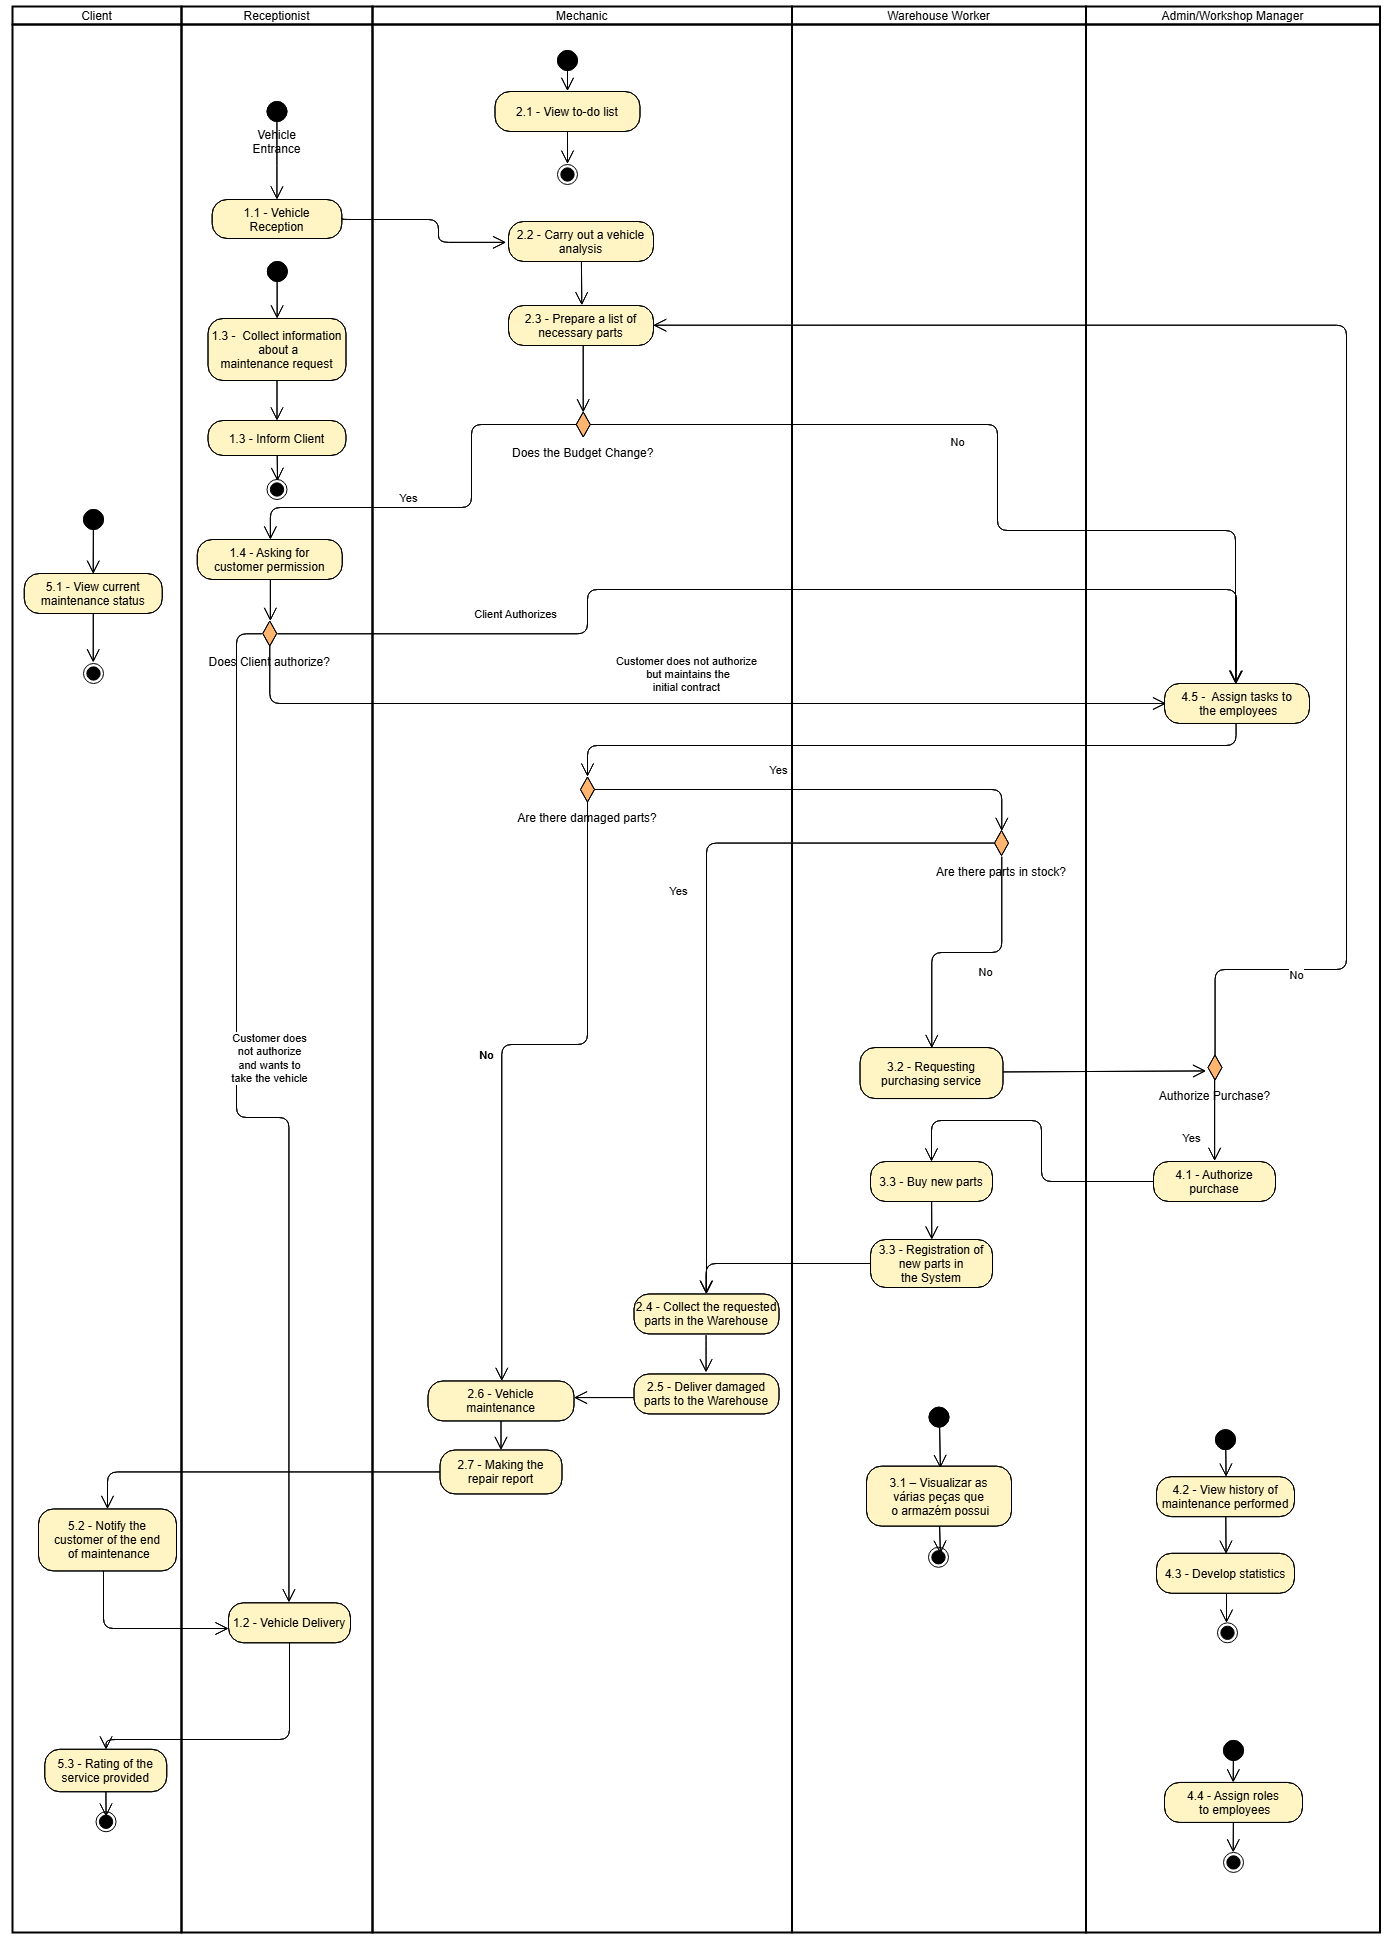
\includegraphics[width=\textwidth]{figs/UseCaseDiagram}
  \label{fig:figure2}
\end{figure}

The system main flow starts when a Client arrives at the dealership for a vehicle maintenance. 
The receptionist get some inputs from the client and decides a Initial budget and check-out date agreed with the Client and insert the information in the system (Use Case 1.1).
After that, a worker will be responsable to the analysis of the vehicle. 
He will add to the system all the problem he finds and the necessary parts that need to be replaced (Use Case 2.2 and 2.3).


If the budget to complete the work or the expected time changes, an alert is sent to the receptionist to inform the Client (Use Case 1.4). 
The result of this interaction must be authorize the changes and continue the work; not authorize the changes but continue as Initially agreed; and 
In the case of the Client not authorizing the changes and wanting to check out the vehicle, the vehicle is delivery and the app will request the client to rate the service (Use Case 1.2 and 5.3). 
If the client does not authorize the changes but wants the maintenance to continue as Initially agreed, the maintenance process continues as if the client authorizing the changes. 
The maintenance process information would only be alterated.
The admin will receive a notification of the new tasks and will assign them to each worker (Use Case 4.5).

From there on, the maintenance process can or can not require the need to a vehicle part to be replaced. 
In the negative case the vehicle goes to the responsable mechanic to do the oil change, tire change, wash, etc (Use Case 2.6). 
In the affirmative case, the Warehouse Operator will check if the parts the mechanic request are available in stock. 
If it does, the operator accepts the request and delivers the parts to the mechanic, which will replace the parts of the vehicle, add it to the system, deliver the damaged parts to the warehouse and do the maintenance (Use Case 2.4, 2.5 and 2.6). 
If it does not, the operator need to buy new parts from the supplier, so he iniciates a new requesting purchase that can be authorized by the admin. 
In the optimal case, the admin accepts the purchase, the operator buy the new parts, register them in the system and delivers them to the mechanic. 
In the worst scenario, the admin reject the purchase and the mechanic needs to request new parts and restart the process (Use Case 2.3).    

Finally, when the vehicle maintenance is finished, the mechanic inserts into the system all operations and tests carried out as well as their results (Use Case 2.7). 
The system notifies the customer that the vehicle is ready for the check out and, when the receptionist delivers the vehicle to the Customer, the client application ask for the client to rate the system (Use Case 5.2, 1.2 and 5.3).

There are also afew secondary flows visible in the figure \ref{fig:figure2}. 
This flows are listed below:
\begin{itemize}
  \item The client enters the aplication to check the status of the maintenance (Use case 5.1);
  \item The mechanic enters the application to view the task he has to do (Use Case 2.1); 
  \item The Warehouse Operator enters the aplication to visualize the diverse parts and components in the warehouse (Use case 3.1); 
  \item The Admin enters the application to assign roles and/or permission to the employees (Use Case 4.4); 
  \item The Admin enters the application to gather information about a maintenance performed and see statistics about tha information (Use Case 4.2 and 4.3); 
\end{itemize}
 









\chapter{Work Plan}%
\label{chapter:workPlan}

\begin{introduction}
In this chapter, i will explain the work plan for the development of the applications and the writing of the dissertation.
\end{introduction} 


\section{Work Plan}

In the next few month i will develop the first version of the applications according to the use cases i defined in the chapter III. 
I will devide the development in 6 two week long sprints, with two contingicy week, one between the sprint 3 and 4 and another after sprint 6 in case of delay of some tasks.

The Sprint 1 will be dedicated to the integration with the System LightMobie System and the development of the Receptionist Use Cases.  

\begin{itemize}
  \item Integration with the Sytem;
  \begin{itemize}
      \item Start Date: 24/01/2025 
      \item End Date: 27/01/2025 
  \end{itemize}
    \item Receptionist use Cases;
    \begin{itemize}
        \item Start Date: 28/01/2025 
        \item End Date: 06/02/2025 
    \end{itemize}
  \end{itemize}

In the Sprint 2, I will be develop the first five Use Cases of the mechanic.  

\begin{itemize}
  \item Mechanic Use cases 2.1 - 2.5;
    \begin{itemize}
      \item Start Date: 07/02/2025 
      \item End Date: 20/02/2025 
  \end{itemize}
\end{itemize}

In the Sprint 3, I will develop the last two Use Cases of the mechanic.  

  \begin{itemize}
    \item Mechanic Use Cases 2.6 and 2.7;
    \begin{itemize}
      \item Start Date: 21/02/2025 
      \item End Date: 06/03/2025 
  \end{itemize}
\end{itemize}

The following week is reserved for the contingicy, so in the case of no delay i can move on to the next sprint, Sprint 4.
In the Sprint 4, I will develop the Admin Use Cases from 4.3 to 4.5. I will skip the 4.1 and 4.2 since they are related to the Warehouse Use Cases.

    \begin{itemize}
      \item Admin Use Cases 4.3 - 4.5;
    \begin{itemize}
      \item Start Date: 14/03/2025 
      \item End Date: 27/03/2025 
  \end{itemize}
\end{itemize}

In the Sprint 5, I will develop remaining two Admin Use Cases, and the Warehouse Use Cases.

\begin{itemize}
  \item Admin Use Cases 4.1 and 4.2;
  \begin{itemize}
    \item Start Date: 28/03/2025 
    \item End Date: 06/04/2025 
  \end{itemize}
  \item Warehouse Use Cases;
  \begin{itemize}
    \item Start Date: 07/04/2025 
    \item End Date: 10/04/2025 
  \end{itemize}
\end{itemize}

In the Sprint 6, I will develop the client application Use Cases.

\begin{itemize}
  \item Client App Use Case;
  \begin{itemize}
    \item Start Date: 11/04/2025  
    \item End Date: 24/05/2025 
  \end{itemize} 
\end{itemize}
The following week is reserved for another contingicy.

  Following de development of the applications, i will reserve a week to conduct a user testing with preferelly users related to the subject.
  The next week i will use to apply the notes and suggestion of the experiment provided to the applications and do some code improvements and testing.
  The remaining time will use to finish writing the dissertation, primarly the results and conclusion.
  The literature will accompany all of this proccess, since it may appear another paper or study that my be relevant to my work.
  This information is illustrated in figure \ref{fig:figure1}.

    \begin{figure}[h]
      \caption{Planned Work described as a Gantt Chart. The master thesis is estimated to be at 25\%, the literature progress to be 70\%, the application Use cases at 85\% and the admin Use Cases at 10\%. The admin Use Cases are at 10\% since they is apart already developed in the LightMobie System.}
      \centering
      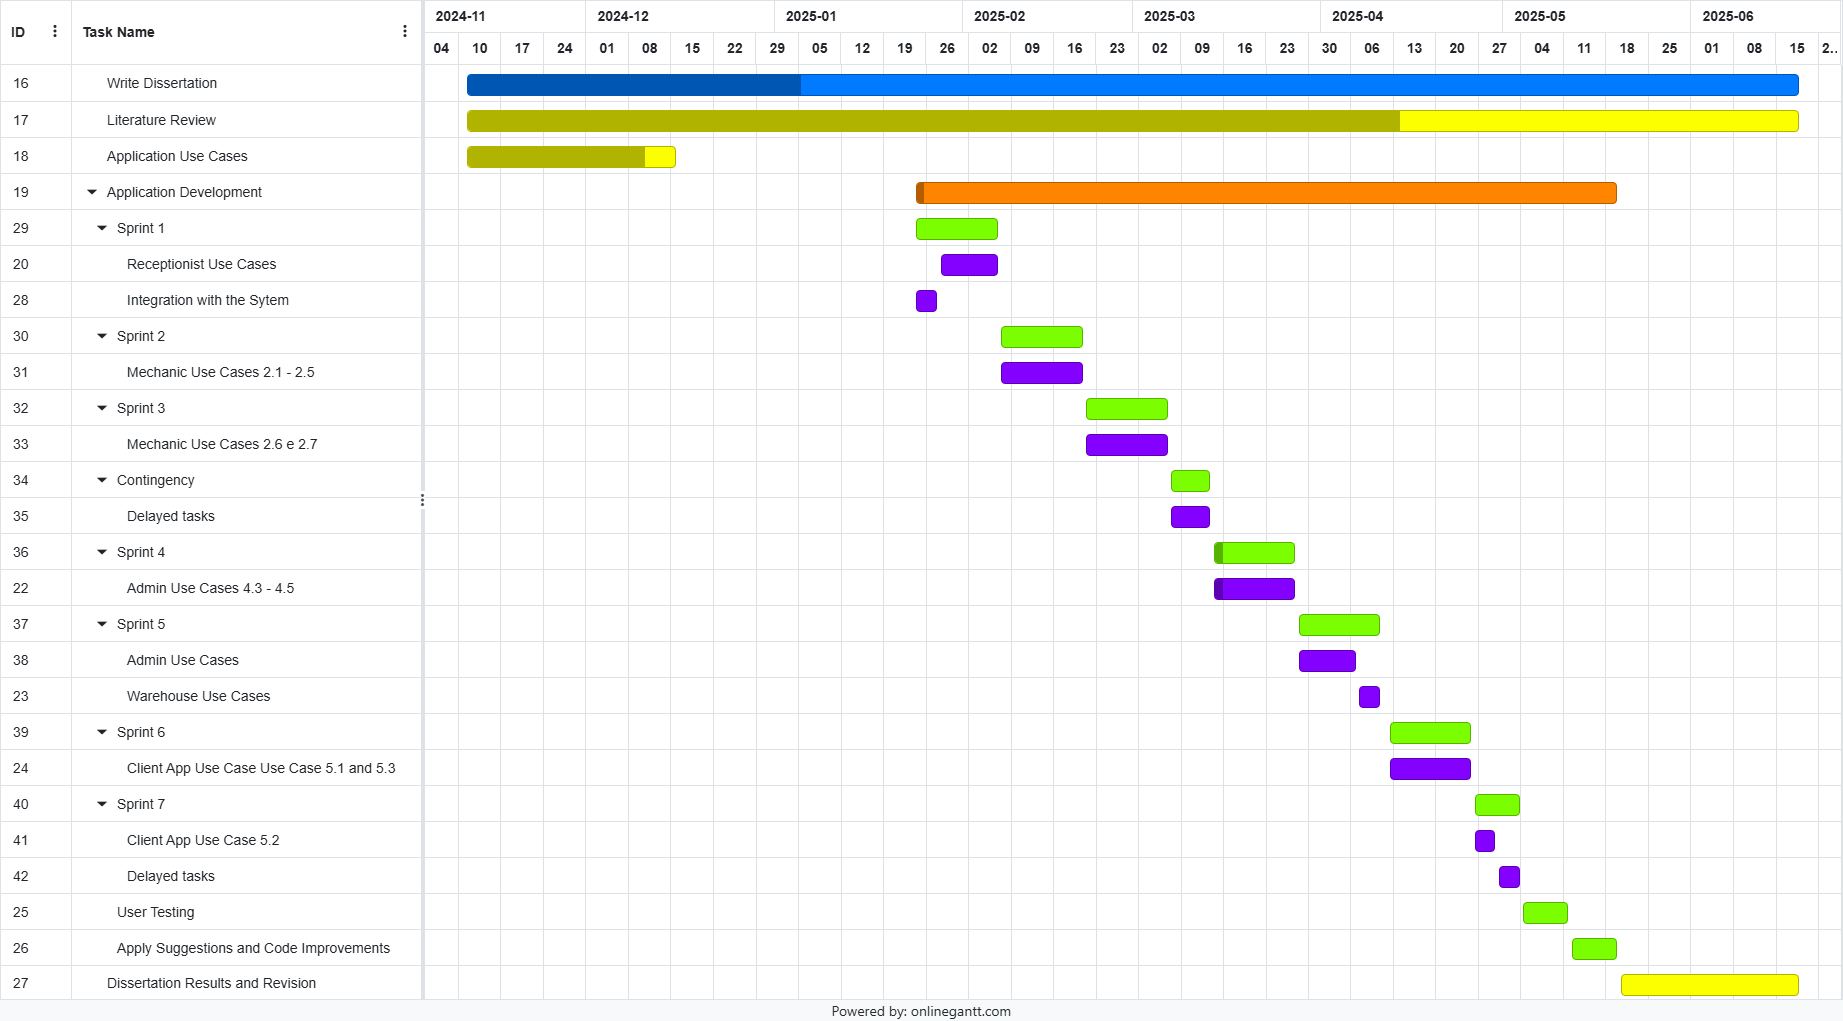
\includegraphics[width=\textwidth]{figs/Gantt}
      \label{fig:figure1}
    \end{figure}

\chapter{Conclusion}%
\label{chapter:conclusion}

\begin{introduction}
The last chapter presents the conclusions of this dissertation.
\end{introduction} 


This dissertation focuses on the planning of the development of a vehicle maintenance web application for LightMobie's dealerships. 
The research on this topic reveals the importance of assuring quality of service in this market, presenting a paper to corroborate this statement.
The paper describes a study made in South Africa using the model SERVQUAL to measure the quality of service in the vehicle maintenance service.
This section also presents a web application using Laravel to increase the performance of the work at a dealership in Libya. 
The results were positive, however, the dealer's workers recommended some improvements to the system.

The development of the web application was based on the workflow of the research paper with an emphasis on quality service evaluation.
The application is also planned to integrate a recommendation from the \citet{MAS_MOTORS}, namely the introduction of an SMS service reminder. 

For the work plan, the use cases were divided into 6 sprints. 
These sprints are two weeks long and have a week interval in the middle and at the end of the development, in case of delays in a few tasks.
After the development of the application, a period is reserved for user testing and adjustments, giving the remaining time to write the dissertation's results.


\section{Future work}

- internal messaging system to comunicate between the rececionist and the mechanics
- adicionar category parts to the administrator
-allow mechanic to do tasks that aren't assigned to him


%\chapter{Literature Review}%
\label{chapter:literatureReview}

\begin{introduction}
The purpose of this chapter is to establish the theoretical and practical foundation for the development of the proposed solution. It begins by examining the vehicle maintenance process, highlighting its relevance to service quality and customer satisfaction. 

Then it incorporates real-world insights gathered from EMEL, the company responsible for operating Lisbon's Gira bike-sharing system. 

Next, it introduces the multiple concepts relevant to the thesis.

And finally, the chapter reviews existing software solutions in the market analyzing their strengths, limitations, and relevance to this dissertation.
\end{introduction} 

To gather relevant information for this topic, I conducted a literature search using the Scopus and Google Scholar platforms. In Scopus, I applied the query “\textit{Vehicle AND Maintenance AND Dealerships}”, which initially returned 49 papers. After a preliminary review of titles and abstracts, 24 were identified as potentially relevant. However, a closer analysis revealed that only three were directly applicable to this dissertation. Many of the discarded papers treated dealerships primarily as sales units of larger companies, which lies outside the scope of this work. Others focused on narrow applications of machine learning, such as predictive maintenance. While valuable in their own right, these approaches did not align with the dissertation's emphasis on web applications and maintenance process management.

A complementary search on Google Scholar yielded three additional studies related to the electric vehicle market in China. Although these works provided useful insights into international contexts, they were excluded as the focus of this dissertation is on maintenance operations rather than market-specific trends.

Ultimately, three papers were selected for detailed analysis. Two of them examined the vehicle maintenance process and highlighted the importance of service quality in ensuring customer satisfaction. The third presented a practical software solution with a use case comparable to the objectives of this dissertation. Together, these studies helped to define the research context and identify key problems and solutions to address during the development phase.

\section{Theoretical Concepts}

\subsection{Vehicle Maintenance}

Delivering vehicle maintenance services involves numerous activities, each crucial for maintaining service quality and ensuring customer satisfaction. 
Any deviation from these activities can negatively impact quality, leading to client dissatisfaction and loyalty loss. ~\cite{Setting_the_after_sale_process}
The loyalty of the client is the main source of income for the company, so it is important to maintain the quality of the service. ~\cite{Setting_the_after_sale_process}
To fulfill this requirement to the fullest, one must supervise every stage of the process. ~\cite{Setting_the_after_sale_process}


\begin{figure}[h]
  \caption{Macro-level Flow of a vehicle maintenance or repair service. This figure was inspired by figure 6: After Sales process from ~\citet{Setting_the_after_sale_process}.}
  \centering
  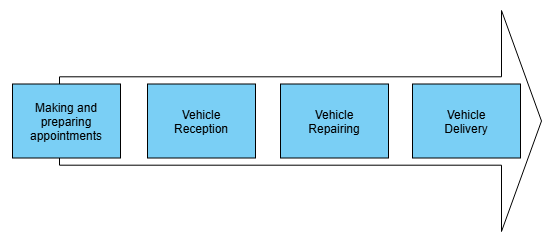
\includegraphics[width=0.50\textwidth]{figs/Vehicle_maintenace_macro}
  \label{fig:Vehicle_maintenace_macro}
\end{figure}

The general flow of vehicle maintenance is illustrated in the figure \ref{fig:Vehicle_maintenace_macro}. 
The first step of the process starts with a client interacting with the garage to schedule a vehicle maintenance or repair. 
After that, the client goes to the garage, where the receptionist receives the client and the vehicle.
Here, the mechanic will perform the maintenance of the vehicle and, when is done, the vehicle will be delivered to the client.

To ensure quality in the first step the receptionist must understand the fill capacity of the garage and the time to complete the job. 
With this information, the rececionist may accurately indicate the time to conclude the vehicle maintenance and get the client trust. ~\cite{Setting_the_after_sale_process}

In the second step, the receptionist and service advisor, when receiving the vehicle, must do a visual confirmation of the vehicle's condition. ~\cite{Setting_the_after_sale_process}
In this step, the receptionist explains to the client the services of the garage and they both agree with the services to be performed until a determined date. ~\cite{Setting_the_after_sale_process}

Following begins the third step and most important phase, the mechanic will perform the maintenance and repair of the vehicle. 
All of this process must be supervised by quality control to ensure that the job is done correctly. ~\cite{Setting_the_after_sale_process}
This includes the repair process, extra work, final tests, and service report. ~\cite{Setting_the_after_sale_process}
To accomplish that the use of a checklist is recommended to ensure precision and accuracy at each step. ~\cite{Setting_the_after_sale_process}

Finally, the last step is the delivery of the vehicle to the client. 
Here, the workshop manager must review the work done and the final price of the service to avoid extra payments from the client and incomplete payments to the workers. ~\cite{Setting_the_after_sale_process}

In this sense, the application of this dissertation will obey this flow.
For the receptionist and mechanic, the application will focus on reducing their mistake by giving accurate and illustrated information and making the work more effective.
And for the workshop manager to control the quality of the service with the assignment of tasks and authorization of purchases. 
Another user will be inserted into this flow, the warehouse operator, to manage the inventory of the dealership. 
The entire flow will be explained in Chapter III. 


\subsection{EMEL}


In June, I visited the company \ac{emel}, an entity responsible for operating and managing the public bike-sharing system Gira in Lisbon. This system comprises approximately 1,800 bicycles and 159 stations, supporting on average 7,405 trips per day, according to 2024 data ~\cite{Gira_Trips}. Each bicycle is scheduled for preventive maintenance either every 50 trips or every 14 days which results in an average of around 70 maintenance operations per day ~\cite{Gira_Maintenance}. This scale of demand requires a well-structured maintenance operation to ensure safety, reliability, and service availability.

To handle this demand, \ac{emel} follows a maintenance workflow that begins when a redistributor identifies a malfunction during routine operations and delivers the vehicle to the workshop. At this stage, the redistributor completes a paper form (Figures \ref{fig:emel_front} and \ref{fig:emel_back}), recording the detected faults and performing a simple diagnostic of electrical components such as the GPS unit and battery. If the vehicle fails these initial tests, it is set aside for a specialist to address before proceeding to standard maintenance. Otherwise, it enters a waiting list until a mechanic becomes available.

When a mechanic is free, the bicycle undergoes repair for both the reported issues and any additional problems detected during inspection. Upon completion, the mechanic records the parts used on the reverse side of the form. The bicycle is then forwarded to a quality control worker for validation. If defects are detected at this stage, the bicycle is returned to the same mechanic for correction before re-entering circulation. Although this process ensures that urgent faults are addressed, the high daily volume of bicycles forces \ac{emel} to prioritize speed over thoroughness, which can result in superficial inspections and undetected secondary issues.

These operational pressures also extend to inventory management. \ac{EMEL} collaborates with multiple suppliers under fixed contracts that specify delivery quantities and deadlines. This information is tracked manually through Excel spreadsheets, which are checked only at periodic intervals. This method provides limited insight into real-time consumption or future requirements. Without digital tools to integrate contract monitoring and inventory tracking, it becomes difficult to anticipate shortages or determine when new tenders should be initiated.

Introducing a digital system that integrates maintenance records with real-time inventory tracking would therefore enable \ac{emel} to optimize its resources, improve oversight, and maintain higher service quality despite the system's large operational scale.


\subsection{Computerized Maintenance Management System}

The software solution i will develop is a \ac{CMMS}.
A \ac{CMMS} is able to centralize and automate the management of maintenance operations, helping the dealership to manage the work tasks and the inventory, providing metrics to optimize the maintenance process.

It maintains a database with the information about the equipment, maintenance schedules, work orders, inventory, and personnel. 
It also document and reports all maintenance actions to facilitate the adherence to the regulatory standards ensuring the quality of the service. 
And analyzes the maintenance costs, downtime, efficiency, and other metrics to improve performence, optimization and reduce cost to the dealership.

The key benefits of the \ac{CMMS} are the improvement of the Preventive Maintenance, since it's easier to analyse the vehicle life and schedule a maintenance before the equipment failures occur; reduce costs, as the life of the vehicle is prolonged and the critical maintenace being avoided, this sofware provides a long-term cost saving; efficiency enhancement, by allowing the workers to focus on completing task instead of paperwork; and Regulatory Compliance, by keeping track and documenting the maintenance activities to comply by the organization standards. 

In conclusion, \ac{CMMS} provides a structured, data-driven approach to maintenance that enhances efficiency, reduces costs, ensures compliance, and ultimately supports the operational reliability of critical equipment and infrastructure.





\subsection{Service Quality}

Service quality is a critical factor in the success of vehicle maintenance services. One widely adopted framework for its evaluation is SERVQUAL, which provides a multidimensional approach for comparing consumers’ perceptions of service quality against their expectations. The model emphasizes five dimensions ~\cite{SERVQUAL_OLD}:


\begin{itemize}
   \item Tangibles – Physical facilities, equipment, and appearance of personnel.
   \item Reliability – Ability to consistently deliver services as promised.
   \item Responsiveness – Willingness to assist the customer and proactivity.
   \item Assurance – Demonstrate courtesy and knowledge and inspire trust and confidence.
   \item Empathy – Caring and treating customers as individuals.
  \end{itemize}

\begin{figure}[h]
  \caption{The 7-point Likert scale where the respondent may answer the question from strongly disagree to strongly agree. ~\cite{master_servqual_model}}
  \centering
  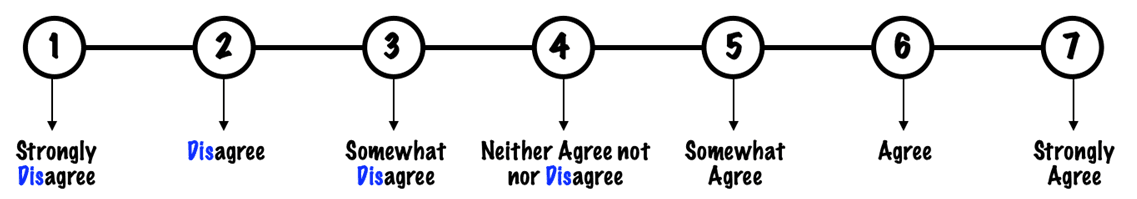
\includegraphics[width=\textwidth]{figs/likert_scale}
  \label{fig:likert_scale}
\end{figure}


To assess these dimensions, SERVQUAL relies on a questionnaire consisting of 22 items, divided across the five categories. Each item requires two ratings: one for the expectation of the service and another for the perception of the service received. The responses are given on a 7-point Likert scale, ranging from strongly disagree to strongly agree, as illustrated in Figure~\ref{fig:likert_scale} ~\cite{Measuring_After_sales_Service_Quality}. The quality gap is determined by the difference between the perception and expectation scores ~\cite{servqual_blog_da_qualidade} ~\cite{Measuring_After_sales_Service_Quality} ~\cite{SERVQUAL_OLD}.

An illustrative application of the SERVQUAL model can be found in the study by ~\citet{Measuring_After_sales_Service_Quality}, which assessed service quality at a CMV SA dealership in South Africa. The authors collected data through semi-structured questionnaires and interviews with customers, managers, and staff. The results, presented in Figure~\ref{fig:SERVQUAL_results}, revealed negative scores across all five dimensions, with an overall average gap of -0.10. These findings highlight that the services provided by the dealership consistently fell short of customer expectations. Among the main suggestions from customers were the expansion of workshops to reduce travel inconvenience and improving the availability of parts, which were often delayed due to international supply chains. The study underscores the importance of continuous service quality monitoring and recommends that dealerships regularly apply the SERVQUAL framework to identify and address performance gaps.

Building on this insight, this dissertation proposes the development of a client-facing application that enables users to evaluate the quality of service received, provide feedback, and make recommendations. This approach follows the SERVQUAL model and aims to strengthen customer trust and satisfaction.
\section{Existing solution}

\subsection{Fiix}
Fiix is a cloud-based \ac{CMMS} that allow organizations to manage their maintenance operations. 
It's main strengths lies on its advanced preventive maintenance scheduling, Comprehensive Work Order and Asset Management and AI-Powered Analytics and Reporting.

Despite the advantages of this software, Fiix has a high learning curve due to it's complexity and not intuitive old-fashion design interface. 
Also Fiix repordly lacks a built-in interal messaging system for crew communication. Most information sharing relies on notes and files attached to work orders, which may not be ideal for real-time collaboration.

With this effects in mind, i will aim in this software development to achieve a simple and user friendly solution where the users can intuitively interact with it by focusing on the key functional feature and easy navigation.

\subsection{Service Management for MAS Motors LLC}
MAS Motors LLC is a Toyota dealership in Libya that provides vehicle maintenance services. The company traditionally relied on manual processes, supported only by basic applications and paper-based documentation. While this approach was manageable at smaller scales, the expansion of the business exposed its inefficiencies and highlighted the need for a more modern solution ~\cite{MAS_MOTORS}. To address this challenge, ~\citet{MAS_MOTORS} developed a web application designed to streamline operations and enhance overall performance at the dealership.

The system was built to support multiple user groups—including service advisers, technicians, and customers—through a centralized platform that manages tasks such as job card handling, inventory updates, and customer service. The application was implemented using Laravel, a PHP web framework, together with MariaDB, an open-source relational database management system.

Evaluation results of the system were generally positive. A survey conducted with employees and customers assessed the solution using the \ac{FURPS} model, yielding scores of 4.27 for functionality, 4.30 for usability, 4.27 for reliability, 4.46 for performance, and 3.36 for supportability. While supportability received the lowest score—mainly due to limited configuration options ~\cite{MAS_MOTORS}—the system overall demonstrated clear improvements in service efficiency and customer satisfaction. Employees also provided valuable recommendations for future enhancements, including SMS-based service reminders, integration with social media platforms, and broader customer configuration options.

Building on these insights, my dissertation incorporates an email notification service, already used in the Lightmobie bike-sharing system, to handle alerts, user validation, and service-related notifications. This addition addresses part of the communication gap identified by MAS Motors employees while leveraging existing infrastructure within the Lightmobie ecosystem.

\subsection{Architecture Comparison}
  
The application will be developed using the ASP.NET Core MVC framework. This choice is motivated by several advantages over Laravel, the framework adopted in the solution proposed by ~\citet{MAS_MOTORS}. A detailed comparison between the two frameworks is presented in Table \ref{table:architetcture_comparison}.

One of the key advantages of ASP.NET Core MVC is its seamless integration with Microsoft SQL databases through the Entity Framework package, which greatly simplifies database interactions. While Laravel also supports relational database integration, ASP.NET Core MVC is generally more suitable for Microsoft environments ~\cite{asp_net_vs_laravel}.

In terms of performance, ASP.NET Core benefits from being based on C\#, a compiled language, whereas Laravel is built on PHP, an interpreted language. This distinction gives ASP.NET Core a performance edge, especially in applications that require scalability and responsiveness.

Security is another critical factor. Although Laravel provides features such as hashing and secure input validation, it requires deeper PHP expertise and continuous monitoring for vulnerabilities. ASP.NET Core, on the other hand, integrates more advanced security mechanisms out of the box, including role-based authentication and login management through the Identity Framework. These abstractions reduce the burden on the developer, allowing greater focus on application functionality ~\cite{asp_net_vs_laravel}.

\begin{table}[]
\begin{tabular}{| m{5em} | m{15em} | m{15em} |}
\hline
Parameter & Laravel & ASP.NET Core MVC \\
\hline
Language & PHP & C\# \\
\hline
Performance & Lower performance due to being an interpreted language & Higher performance due to being a compiled language \\
\hline 
Security & Provides features such as hashing and input validation, but requires strong PHP knowledge and manual management & Offers advanced built-in security tools, including role-based authentication and Identity Framework support \\
\hline
Integration with SQL & Supports various relational databases & Recommended for Microsoft environments due to strong integration packages \\
\hline
\end{tabular}
\caption{Comparison between Laravel and ASP.NET Core MVC frameworks for integration into the Lightmobie platform.}
\label{table:architetcture_comparison}
\end{table}
 
Another strong motivation for adopting ASP.NET Core MVC is its compatibility with Lightmobie's Fleet Management System, which follows the same architectural approach. This ensures easier integration, particularly for functionalities such as authentication and role assignment, which are already implemented and can be reused. While this choice may introduce some additional complexity, my prior involvement in developing the Fleet Management System provides familiarity with its features, thereby reducing the learning curve and facilitating a smoother integration process.
  

\section{Conclusion}

In this chapter i explained the theoretical concepts of the vehicle maintenance process in the literature and in the real case example EMEL in lisbon, and The SERVQUAL method to evaluate the quality of the service of a organization.
I also describe the existing solutions in the market, namely Fiix, and the results of MAS Motors LLC's application.
This solutions lack a intuitive interface and a notification service, so in this dissertation i will focus on accomplish that.


%\chapter{Methodology}%
\label{chapter:methodology}

\begin{introduction}
In this chapter, i will present the non functional requirements of the applications, as well as the use cases of the user that will interact with them. 
\end{introduction} 




\section{Applications Requirements} 


To identify the requirements of the application, i used the FURPS model. 
The non functional requirements are listed below:

\begin{itemize}
  \item Scalability – The system should be able to handle 500 users simultaneously without degradading the performance.
  \item Reliability – The system should have a high availability of 99\% and the system also should not take longer then 4 hours to recover from a failure.
  \item Performance – The system should not take longer then 2 seconds to respond.
  \item Usability – The train of a new user should not take longer then 8 hours.
  \item Supportability – The system should be suported on the web browsers Chrome, Firefox, Microsoft Edge and Safari.
\end{itemize}

For the functional requirements of the applications, i developed a set of use cases for each user.
The structure of the dealership application was based on the work of the author ~\citet{Setting_the_after_sale_process} and is separated into 4 key user roles: receptionist, mechanic, warehouse operator and administrator.

The receptionist will be responsable to interact with the client, this includes the vehicle check-in and check-out and user comunication in the case of changes in the Initial stablished price and vehicle actions. 
The Use cases of the receptionist are:

\begin{itemize}
    \item Use Case 1.1 – Vehicle Reception
    \begin{itemize}
      \item Scenario – Client arrives at the dealership with a vehicle to be repaired.
      \item Objective – Create a new maintenance request in the system.
      \item System – The receptionist insert in the a form all the information about the initial maintenance request from the client and vehicle and creates a new maintenance request with the date and budget agreed with the client 
    \end{itemize}
    \item Use Case 1.2 – Vehicle Delivery 
    \begin{itemize}
      \item Scenario – The Receptionist delivered the vehicle to the Client.
      \item Objective – Complete the vehicle maintenance process.
      \item System – Sends a report in a pdf format to the client with the information of the maintenance request and alters the maintenance request status in the system to concluded. 
    \end{itemize}
    \item Use Case 1.3 – Collect information about a maintenance request
    \begin{itemize}
      \item Scenario – A Client call the dealership to ask about the maintenance of his vehicle.
      \item Objective – Visualize the maintenance information.
      \item System –  The Receptionist searches a list of maintenance requests by vehicle/customer name/maintenance ID and, by clicking on the element details button, he can view the maintenance details.
    \end{itemize}
    \item Use Case 1.4 – Asking for customer permission
    \begin{itemize}
      \item Scenario – O problem in a vehicle maintenance has occurred and the Initial agreement with client may be broken.
      \item Objective – Inform the client of the problem and achieve an agreement.
      \item System – The Receptionist receives an alert that there has been a change in the initial maintenance budget for a vehicle and/or a change in the maintenance completion deadline, so he needs to contact the customer to inform him. Depending on customer feedback, the receptionist accepts the request, declines the request or terminates the maintenance.
    \end{itemize}
  \end{itemize}  
  \hfill \break


  The mechanic will be responsable to do the maintenance in the vehicle, like oil change, tire change, trade vehicle parts, etc. 
  It will previously evaluate the vehicle, to assure the Initial evaluation of the receptionist is not lacking, and after the maintenance is done, it will write a report of the operations done. 
  The Mechanic Use cases are:

  \begin{itemize}
    \item Use Case 2.1 – View to-do list
    \begin{itemize}
      \item Scenario – The mechanic arrives at dealership and wants to see what tasks he has to do today.
      \item Objective – See the day's work organization.
      \item System – The mechanic watches a list of tasks that were assign from the administrator, as soon as he enters the system. Each task is accompany by a description, a priority, the vehicle identification, a set of actions to be performed and comments from other users. 
    \end{itemize}
    \item Use Case 2.2 – Carry out a vehicle analysis 
    \begin{itemize}
      \item Scenario – A new vehicle needs to be analyzed.
      \item Objective – Confirm the Initial analysis of the receptionist and search for additional problems.
      \item System – The mechanic enters the problems he finds in the vehicle into the system. 
    \end{itemize}
    \item Use Case 2.3 – Prepare a list of necessary parts
    \begin{itemize}
      \item Scenario – After vehicle analysis.
      \item Objective – Elaborate a request of vehicle parts for the warehouse.
      \item System – The mechanic selects the parts of the vehicle that need to be replaced and sends a request with the new parts to the warehouse.
    \end{itemize}
    \item Use Case 2.4 – Collect the requested parts in the Warehouse
    \begin{itemize}
      \item Scenario – The mechanic goes to the warehouse to collect new parts for the vehicle.
      \item Objective – Collect parts to replace the damaged parts in the vehicle.
      \item System – The mechanic add the new parts to the vehicle in the system.
    \end{itemize}
    \item Use Case 2.5 – Deliver damaged parts to the Warehouse
    \begin{itemize}
      \item Scenario – The mechanic goes to the warehouse to deliver the damaged parts.
      \item Objective – Register the parts as being damaged.
      \item System – The mechanic removes the damaged parts from the vehicle and change the status to damaged.
    \end{itemize}
\item Use Case 2.6 – Vehicle maintenance
\begin{itemize}
  \item Scenario – A new vehicle is ready for a maintenance.
  \item Objective – The mechanic will do the vehicle maintenance (oil change, tire change, vehicle wash…).
  \item System – The mechanic sees a set of tasks that he needs to do to complete the vehicle maintenance and whenever he finishes a task, he marks it as completed.
\end{itemize}
\item Use Case 2.7 – Making the repair report
\begin{itemize}
  \item Scenario – After vehicle maintenance.
  \item Objective – Conclude the maintenance of a vehicle.
  \item System – The Mechanic enters into the system all operations and tests carried out on the system as well as their results.
\end{itemize}
\end{itemize}
\hfill \break

The warehouse operator is responsable to manage the dealer's stock and ask for suplies, so i write the following use cases:

\begin{itemize}
  \item Use Case 3.1 – View the different parts that the warehouse possess
  \begin{itemize}
    \item Scenario – The warehouse worker wants to view the quantity of a certain parts that the warehouse possess.
    \item Objective – Show quantitative warehouse information.
    \item System – List of all parts and their quantities that the warehouse possess. 
  \end{itemize}
  \item Use Case 3.2 – Requesting purchasing service 
  \begin{itemize}
    \item Scenario – The warehouse worker discovers that he has an insufficient number of parts for maintenance or anticipates that this part will be missing soon.
    \item Objective – Request permission to purchase parts from the supplier.
    \item System – The Warehouse Worker will place a purchase order for parts. The system notifies the administrator via the platform and by email requesting authorization to do the purchase. 
  \end{itemize}
  \item Use Case 3.3 – Registration of new parts in the System
  \begin{itemize}
    \item Scenario – The warehouse purchased several parts from a supplier.
    \item Objective – Register new parts in the system.
    \item System – Warehouse operator adds a specific type of part to the system with its appropriate description and identification.
  \end{itemize}
\end{itemize}
\hfill \break

The last user of the application is the administrator or Workshop Manager. This user is in charge of managing the platform and the dealership. So the main use cases I encountered are:

\begin{itemize}
  \item Use Case 4.1 – Authorizing purchases
  \begin{itemize}
    \item Scenario –  The administrator received a purchase request.
    \item Objective – Authorize or reject a purchase authorization request.
    \item System – List of all purchase authorization requests, as well as their details. The administrator can change the status of this request, rejecting or authorizing. 
  \end{itemize}
  \item Use Case 4.2 – View history of maintenance performed
  \begin{itemize}
    \item Scenario – The administrator wants to gather information from recently performed maintenance.
    \item Objective – View information about a specific maintenance that occurred.
    \item System – List of all maintenance that occurred as well as its details (who carried it out, which parts were removed, the name of the customer, tests carried out and their results…). 
  \end{itemize}
  \item Use Case 4.3 – Develop statistics
  \begin{itemize}
    \item Scenario – The administrator wants to gather statistics on maintenance that was carried out in the last month.
    \item Objective – View information about maintenance over a given period of time.
    \item System – Presentation of the number of parts replaced, number of purchases, total price spent on new parts, remuneration for maintenance, average customer's rating, etc.
  \end{itemize}
  \item Use Case 4.4 – Assign roles to employees
  \begin{itemize}
    \item Scenario – A new employee has been hired.
    \item Objective –  Assign roles to new employee.
    \item System – The administrator assigns the new employee a certain role and set of permissions.
  \end{itemize}
  \item Use Case 4.5 – Assign tasks to the employees
  \begin{itemize}
    \item Scenario – A new maintenance request has been requested.
    \item Objective – Assign and organize tasks to different employees.
    \item System – The administrator assigns the various stages of vehicle maintenance to the various workshop employees.
  \end{itemize}
\end{itemize}
\hfill \break

The client application will only be interacted by a role of users, the client.
The use cases are listed below:

\begin{itemize}
  \item Use Case 5.1 – View current maintenance status
  \begin{itemize}
    \item Scenario – The Customer wants to find information regarding the vehicle maintenance procedure.
    \item Objective – Display current maintenance status.
    \item System – The system will illustrate all the maintenance steps that the vehicle has already undergone, as well as those that remain to be completed. 
  \end{itemize}
  \item Use Case 5.2 – Notify the customer of the end of maintenance 
  \begin{itemize}
    \item Scenario – Vehicle maintenance has been completed and the customer can now collect the vehicle.
    \item Objective – Notify the user of the end of maintenance.
    \item System – The system will show a native notification on the customer's cell phone informing that the vehicle is ready to be picked up. 
  \end{itemize}
  \item Use Case 5.3 – Rating of the service provided
  \begin{itemize}
    \item Scenario – The client receives the vehicle and the receptionist completes the maintenance process.
    \item Objective – Get feedback from the client.
    \item System – The system will show a form to the client asking about service provided. The crucial points are time of the service, service quality, user interaction and price.
  \end{itemize}
\end{itemize}
\hfill \break

With this requirements, both application should increase the efficiency of the work at the dealership and improve client loyalty to ensure profit.


\section{Applications Workflow}

After the development of the use cases i designed a flow chart to understand the users' interaction with the system and each other. The chart is visible in figure \ref{fig:figure2}.

\begin{figure}[h]
  \caption{Use Case Flow Chart of the Client, Receptionist, Mechanic, Warehouse Operator and administrator.}
  \centering
  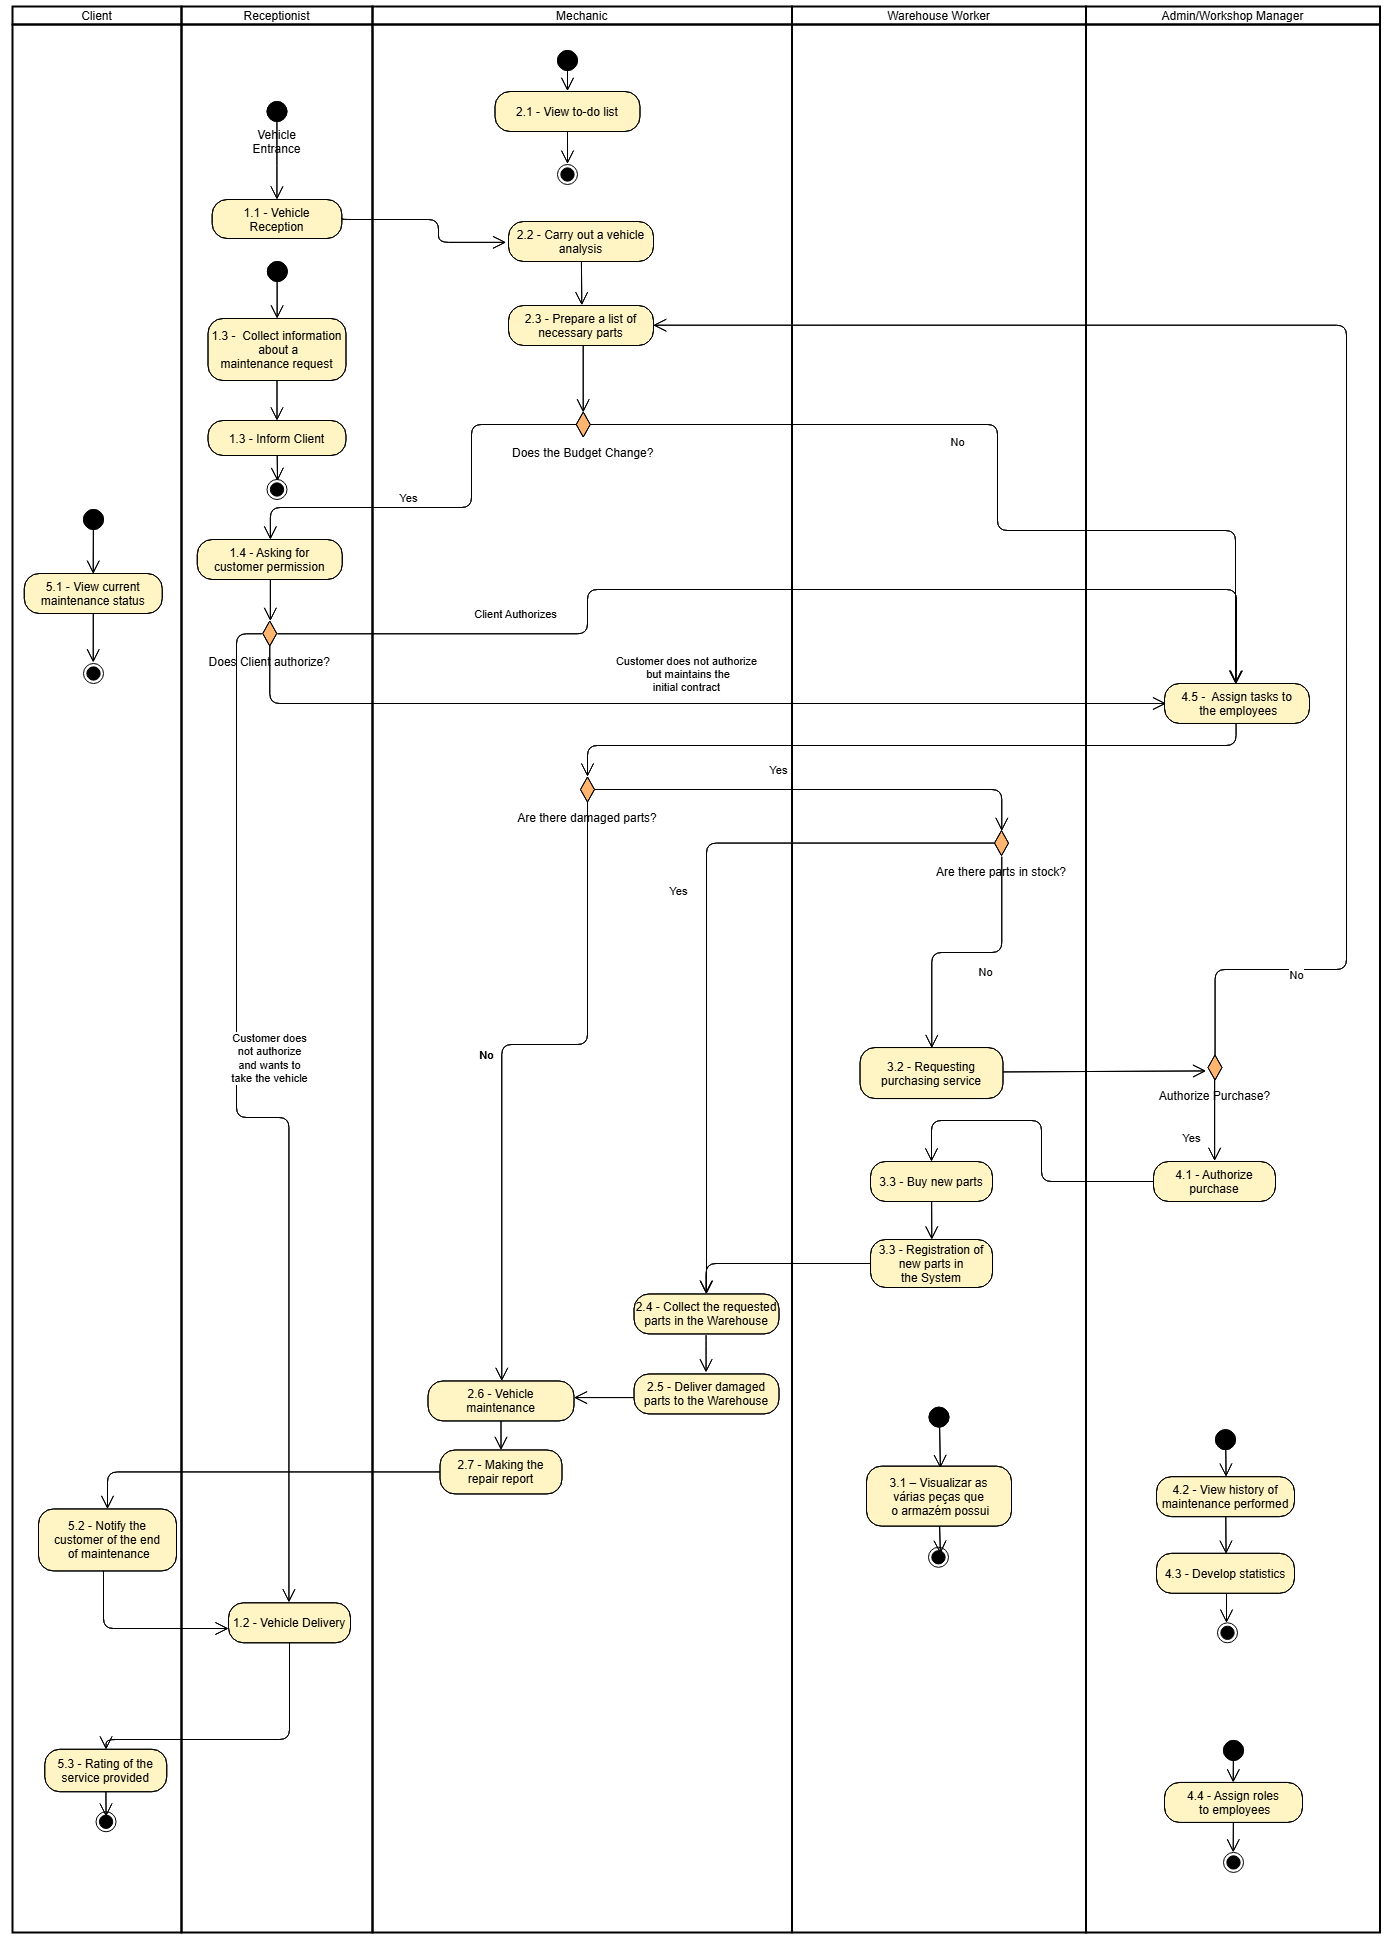
\includegraphics[width=\textwidth]{figs/UseCaseDiagram}
  \label{fig:figure2}
\end{figure}

The system main flow starts when a Client arrives at the dealership for a vehicle maintenance. 
The receptionist get some inputs from the client and decides a Initial budget and check-out date agreed with the Client and insert the information in the system (Use Case 1.1).
After that, a worker will be responsable to the analysis of the vehicle. 
He will add to the system all the problem he finds and the necessary parts that need to be replaced (Use Case 2.2 and 2.3).


If the budget to complete the work or the expected time changes, an alert is sent to the receptionist to inform the Client (Use Case 1.4). 
The result of this interaction must be authorize the changes and continue the work; not authorize the changes but continue as Initially agreed; and 
In the case of the Client not authorizing the changes and wanting to check out the vehicle, the vehicle is delivery and the app will request the client to rate the service (Use Case 1.2 and 5.3). 
If the client does not authorize the changes but wants the maintenance to continue as Initially agreed, the maintenance process continues as if the client authorizing the changes. 
The maintenance process information would only be alterated.
The admin will receive a notification of the new tasks and will assign them to each worker (Use Case 4.5).

From there on, the maintenance process can or can not require the need to a vehicle part to be replaced. 
In the negative case the vehicle goes to the responsable mechanic to do the oil change, tire change, wash, etc (Use Case 2.6). 
In the affirmative case, the Warehouse Operator will check if the parts the mechanic request are available in stock. 
If it does, the operator accepts the request and delivers the parts to the mechanic, which will replace the parts of the vehicle, add it to the system, deliver the damaged parts to the warehouse and do the maintenance (Use Case 2.4, 2.5 and 2.6). 
If it does not, the operator need to buy new parts from the supplier, so he iniciates a new requesting purchase that can be authorized by the admin. 
In the optimal case, the admin accepts the purchase, the operator buy the new parts, register them in the system and delivers them to the mechanic. 
In the worst scenario, the admin reject the purchase and the mechanic needs to request new parts and restart the process (Use Case 2.3).    

Finally, when the vehicle maintenance is finished, the mechanic inserts into the system all operations and tests carried out as well as their results (Use Case 2.7). 
The system notifies the customer that the vehicle is ready for the check out and, when the receptionist delivers the vehicle to the Customer, the client application ask for the client to rate the system (Use Case 5.2, 1.2 and 5.3).

There are also afew secondary flows visible in the figure \ref{fig:figure2}. 
This flows are listed below:
\begin{itemize}
  \item The client enters the aplication to check the status of the maintenance (Use case 5.1);
  \item The mechanic enters the application to view the task he has to do (Use Case 2.1); 
  \item The Warehouse Operator enters the aplication to visualize the diverse parts and components in the warehouse (Use case 3.1); 
  \item The Admin enters the application to assign roles and/or permission to the employees (Use Case 4.4); 
  \item The Admin enters the application to gather information about a maintenance performed and see statistics about tha information (Use Case 4.2 and 4.3); 
\end{itemize}
 









%\chapter{Work Plan}%
\label{chapter:workPlan}

\begin{introduction}
In this chapter, i will explain the work plan for the development of the applications and the writing of the dissertation.
\end{introduction} 


\section{Work Plan}

In the next few month i will develop the first version of the applications according to the use cases i defined in the chapter III. 
I will devide the development in 6 two week long sprints, with two contingicy week, one between the sprint 3 and 4 and another after sprint 6 in case of delay of some tasks.

The Sprint 1 will be dedicated to the integration with the System LightMobie System and the development of the Receptionist Use Cases.  

\begin{itemize}
  \item Integration with the Sytem;
  \begin{itemize}
      \item Start Date: 24/01/2025 
      \item End Date: 27/01/2025 
  \end{itemize}
    \item Receptionist use Cases;
    \begin{itemize}
        \item Start Date: 28/01/2025 
        \item End Date: 06/02/2025 
    \end{itemize}
  \end{itemize}

In the Sprint 2, I will be develop the first five Use Cases of the mechanic.  

\begin{itemize}
  \item Mechanic Use cases 2.1 - 2.5;
    \begin{itemize}
      \item Start Date: 07/02/2025 
      \item End Date: 20/02/2025 
  \end{itemize}
\end{itemize}

In the Sprint 3, I will develop the last two Use Cases of the mechanic.  

  \begin{itemize}
    \item Mechanic Use Cases 2.6 and 2.7;
    \begin{itemize}
      \item Start Date: 21/02/2025 
      \item End Date: 06/03/2025 
  \end{itemize}
\end{itemize}

The following week is reserved for the contingicy, so in the case of no delay i can move on to the next sprint, Sprint 4.
In the Sprint 4, I will develop the Admin Use Cases from 4.3 to 4.5. I will skip the 4.1 and 4.2 since they are related to the Warehouse Use Cases.

    \begin{itemize}
      \item Admin Use Cases 4.3 - 4.5;
    \begin{itemize}
      \item Start Date: 14/03/2025 
      \item End Date: 27/03/2025 
  \end{itemize}
\end{itemize}

In the Sprint 5, I will develop remaining two Admin Use Cases, and the Warehouse Use Cases.

\begin{itemize}
  \item Admin Use Cases 4.1 and 4.2;
  \begin{itemize}
    \item Start Date: 28/03/2025 
    \item End Date: 06/04/2025 
  \end{itemize}
  \item Warehouse Use Cases;
  \begin{itemize}
    \item Start Date: 07/04/2025 
    \item End Date: 10/04/2025 
  \end{itemize}
\end{itemize}

In the Sprint 6, I will develop the client application Use Cases.

\begin{itemize}
  \item Client App Use Case;
  \begin{itemize}
    \item Start Date: 11/04/2025  
    \item End Date: 24/05/2025 
  \end{itemize} 
\end{itemize}
The following week is reserved for another contingicy.

  Following de development of the applications, i will reserve a week to conduct a user testing with preferelly users related to the subject.
  The next week i will use to apply the notes and suggestion of the experiment provided to the applications and do some code improvements and testing.
  The remaining time will use to finish writing the dissertation, primarly the results and conclusion.
  The literature will accompany all of this proccess, since it may appear another paper or study that my be relevant to my work.
  This information is illustrated in figure \ref{fig:figure1}.

    \begin{figure}[h]
      \caption{Planned Work described as a Gantt Chart. The master thesis is estimated to be at 25\%, the literature progress to be 70\%, the application Use cases at 85\% and the admin Use Cases at 10\%. The admin Use Cases are at 10\% since they is apart already developed in the LightMobie System.}
      \centering
      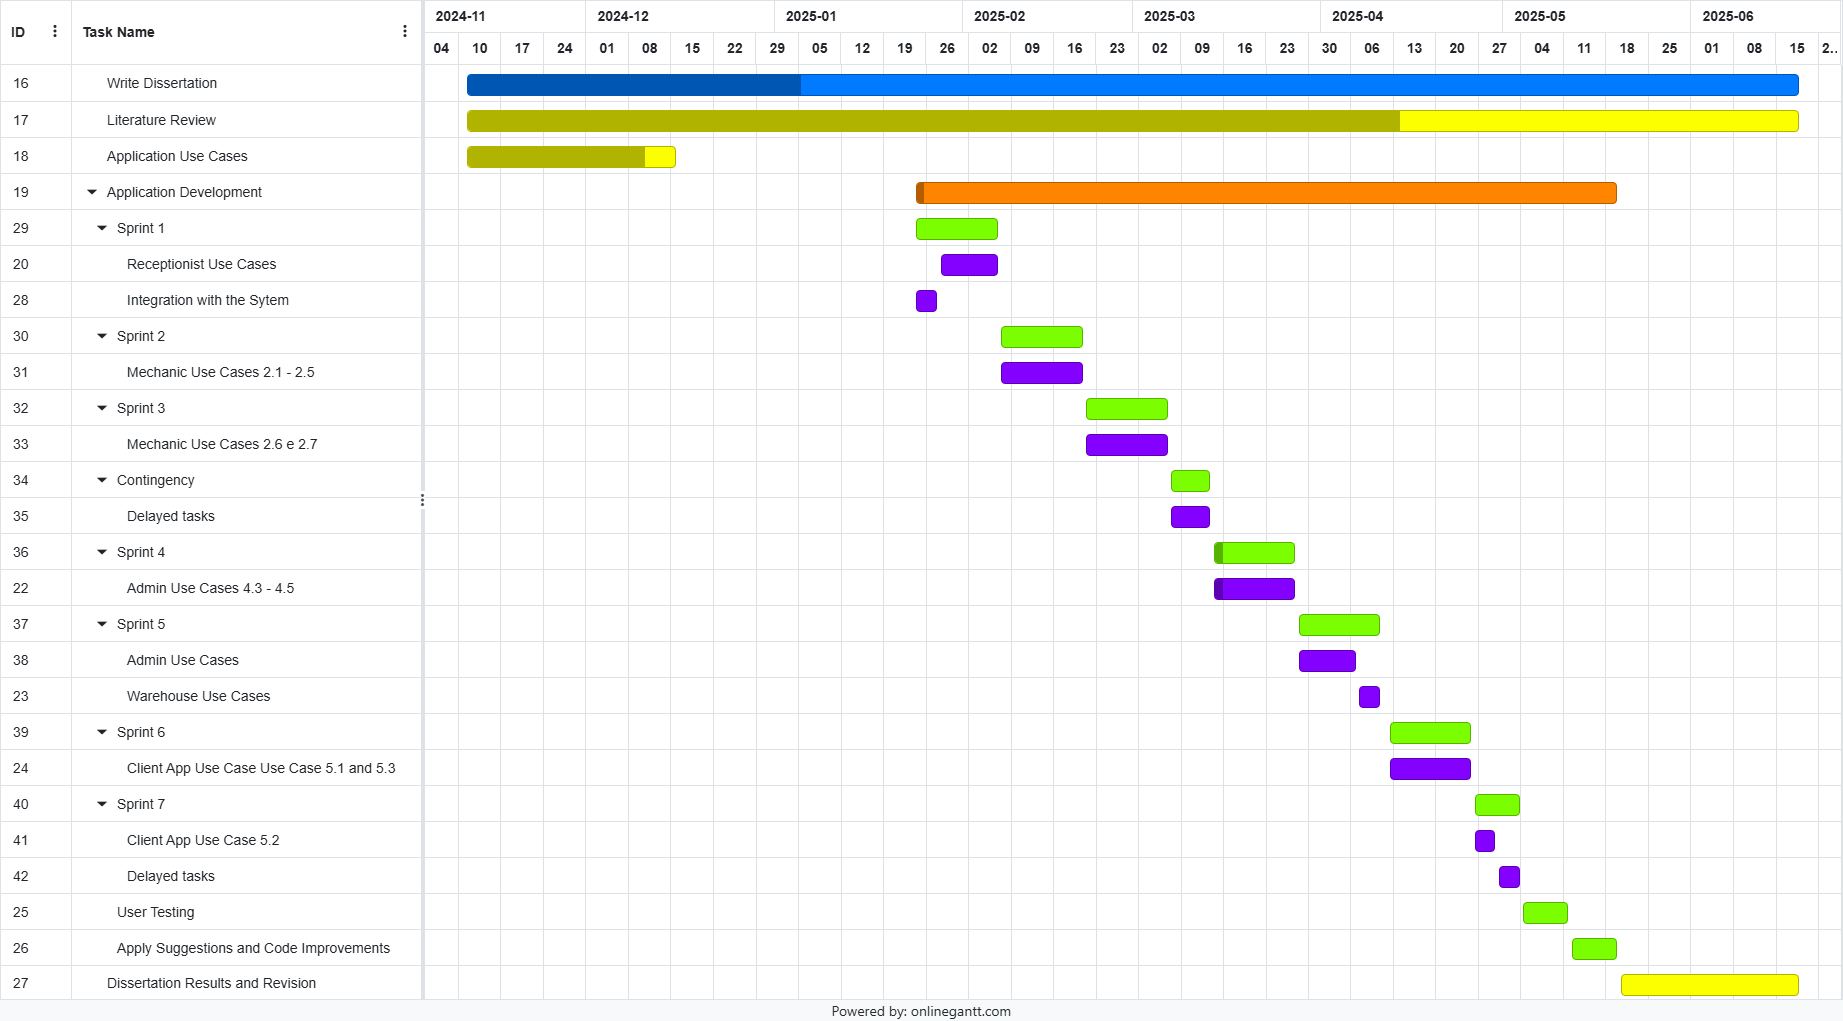
\includegraphics[width=\textwidth]{figs/Gantt}
      \label{fig:figure1}
    \end{figure}


%%%%%%%%%%%%%%%%%%%%%%%%%%%%%%%%%%%%%%%%%%%%%%%%%%%%%%%
% End of Thesis text 
%%%%%%%%%%%%%%%%%%%%%%%%%%%%%%%%%%%%%%%%%%%%%%%%%%%%%%%

\backmatter

%%%%%%%%%%%%%%%%%%%%%%%%%%%%%%%%%%%%%%%%%%%%%%%%%%%%%%%
% Print all used references
%%%%%%%%%%%%%%%%%%%%%%%%%%%%%%%%%%%%%%%%%%%%%%%%%%%%%%%

\begingroup
\renewcommand{\bibfont}{\footnotesize}
% Redefine References name to Portuguese
% Change if you are using english
\defbibheading{bibliography}[References]{
	\chapter{#1}
}
\SingleSpacing
\setlength\bibitemsep{8pt}
\printbibliography[heading=bibliography]
\endgroup


%%%%%%%%%%%%%%%%%%%%%%%%%%%%%%%%%%%%%%%%%%%%%%%%%%%%%%%
% Load appendix
%%%%%%%%%%%%%%%%%%%%%%%%%%%%%%%%%%%%%%%%%%%%%%%%%%%%%%%

\mainmatterWithoutReset
\appendix

\chapter{Additional content}


\begin{figure}[htbp]
  \caption{Front page of the paper form used by \acs{emel} during vehicle maintenance. Operators use this section to record identified malfunctions.}
  \centering
  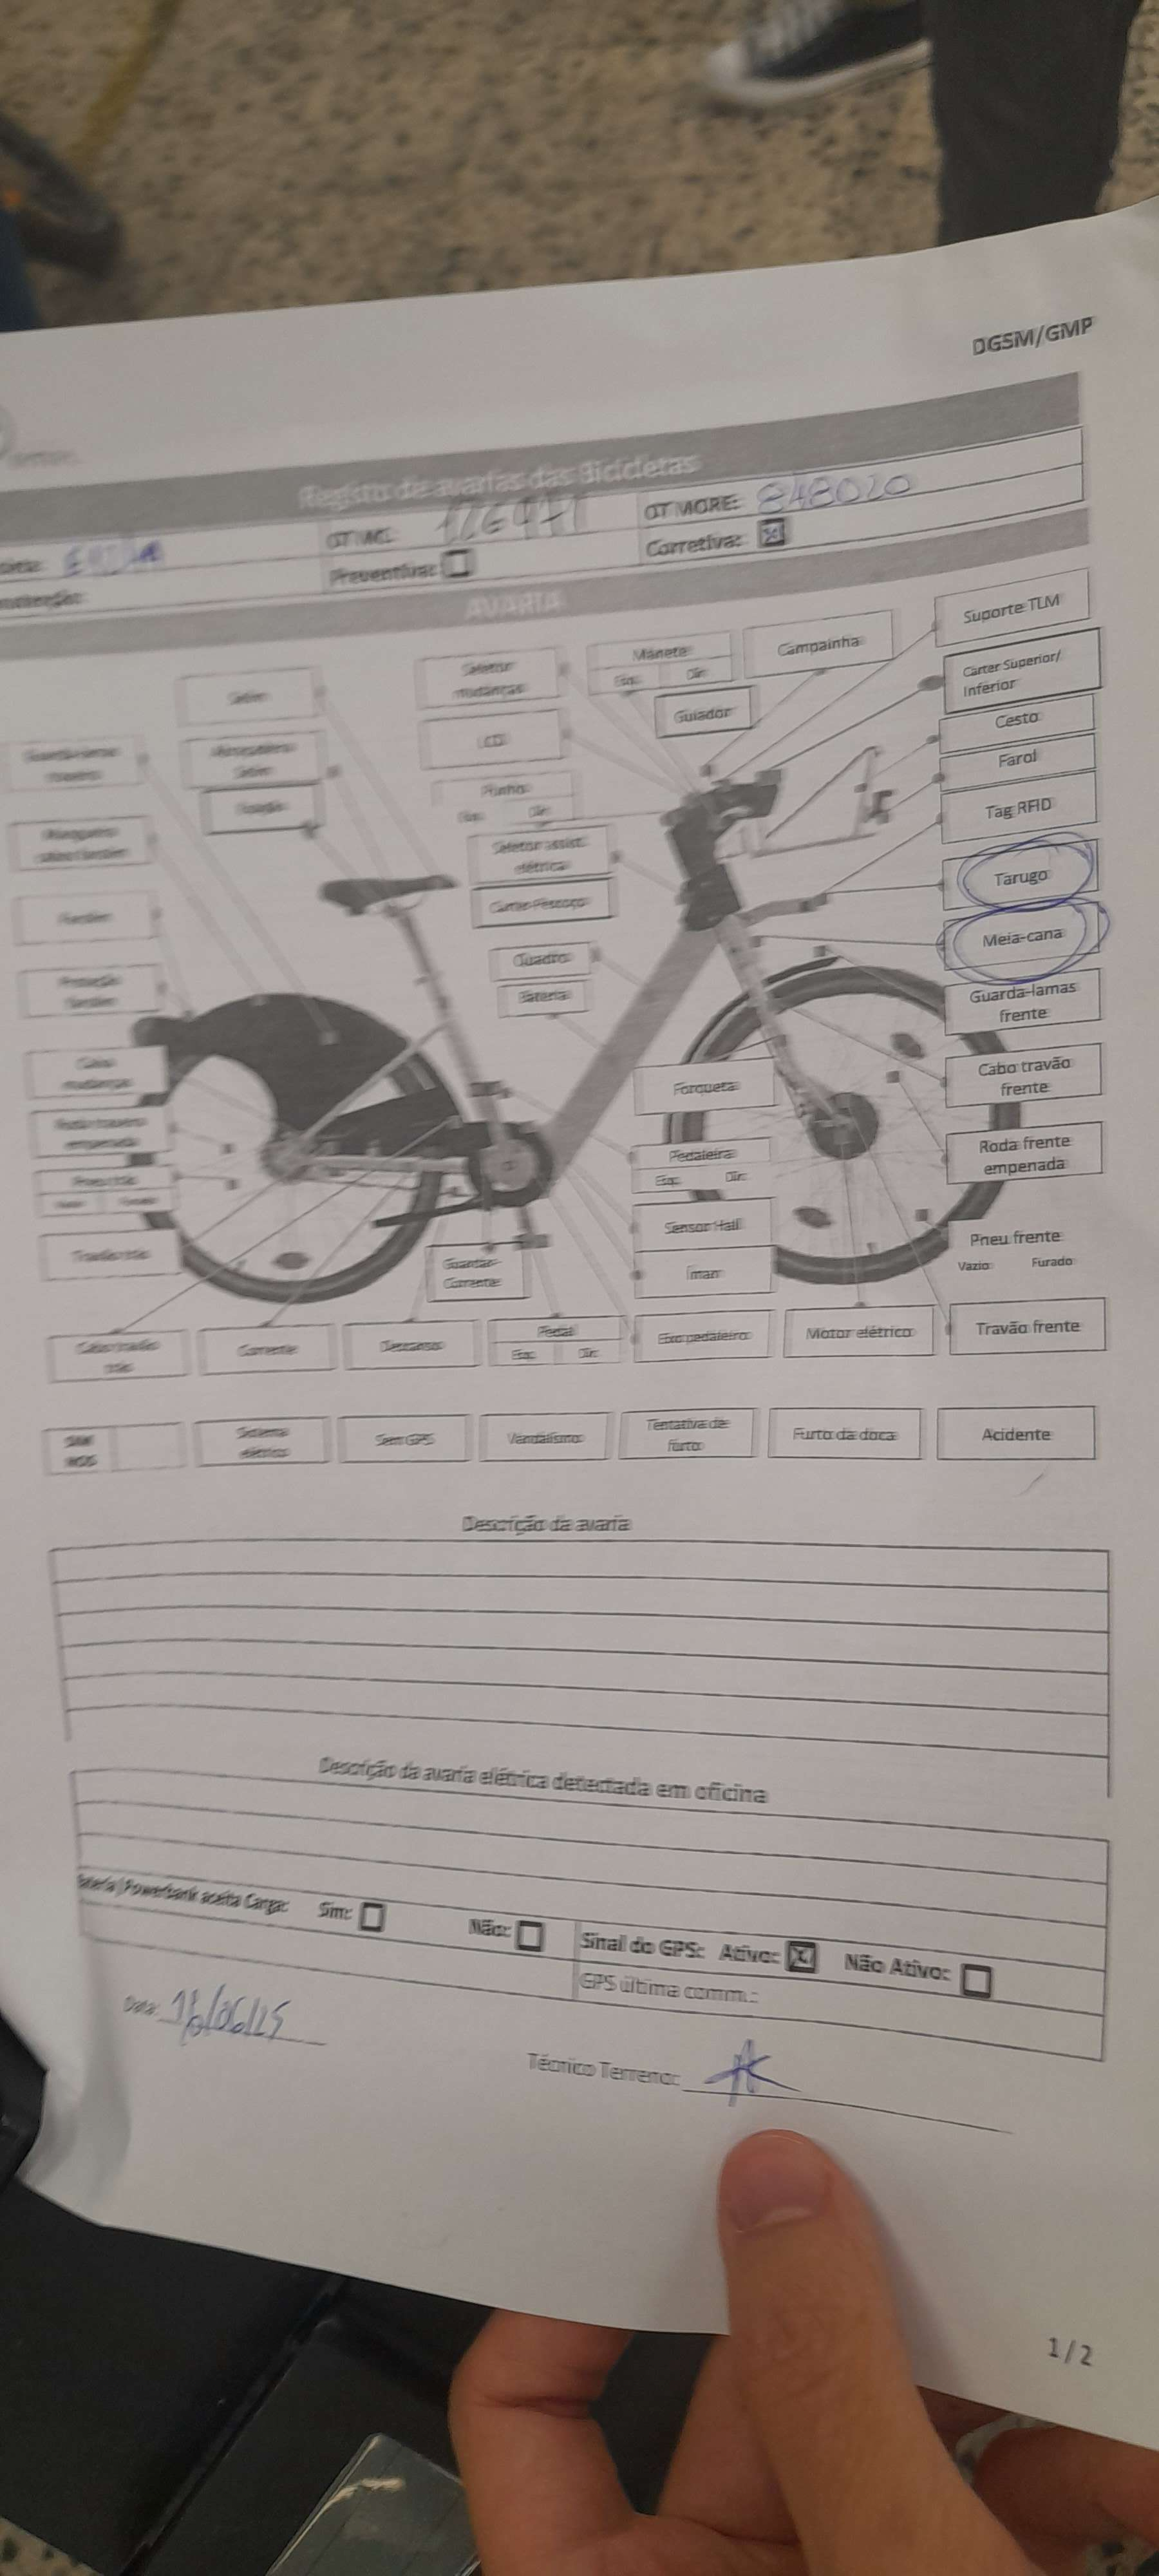
\includegraphics[width=0.50\textwidth]{figs/chapter2/emel_front}
  \label{fig:emel_front}
\end{figure}

\begin{figure}[htbp]
  \caption{Back page of the paper form used by \acs{emel} during vehicle maintenance. Mechanics use this section to document the parts replaced during the repair process.}
  \centering
  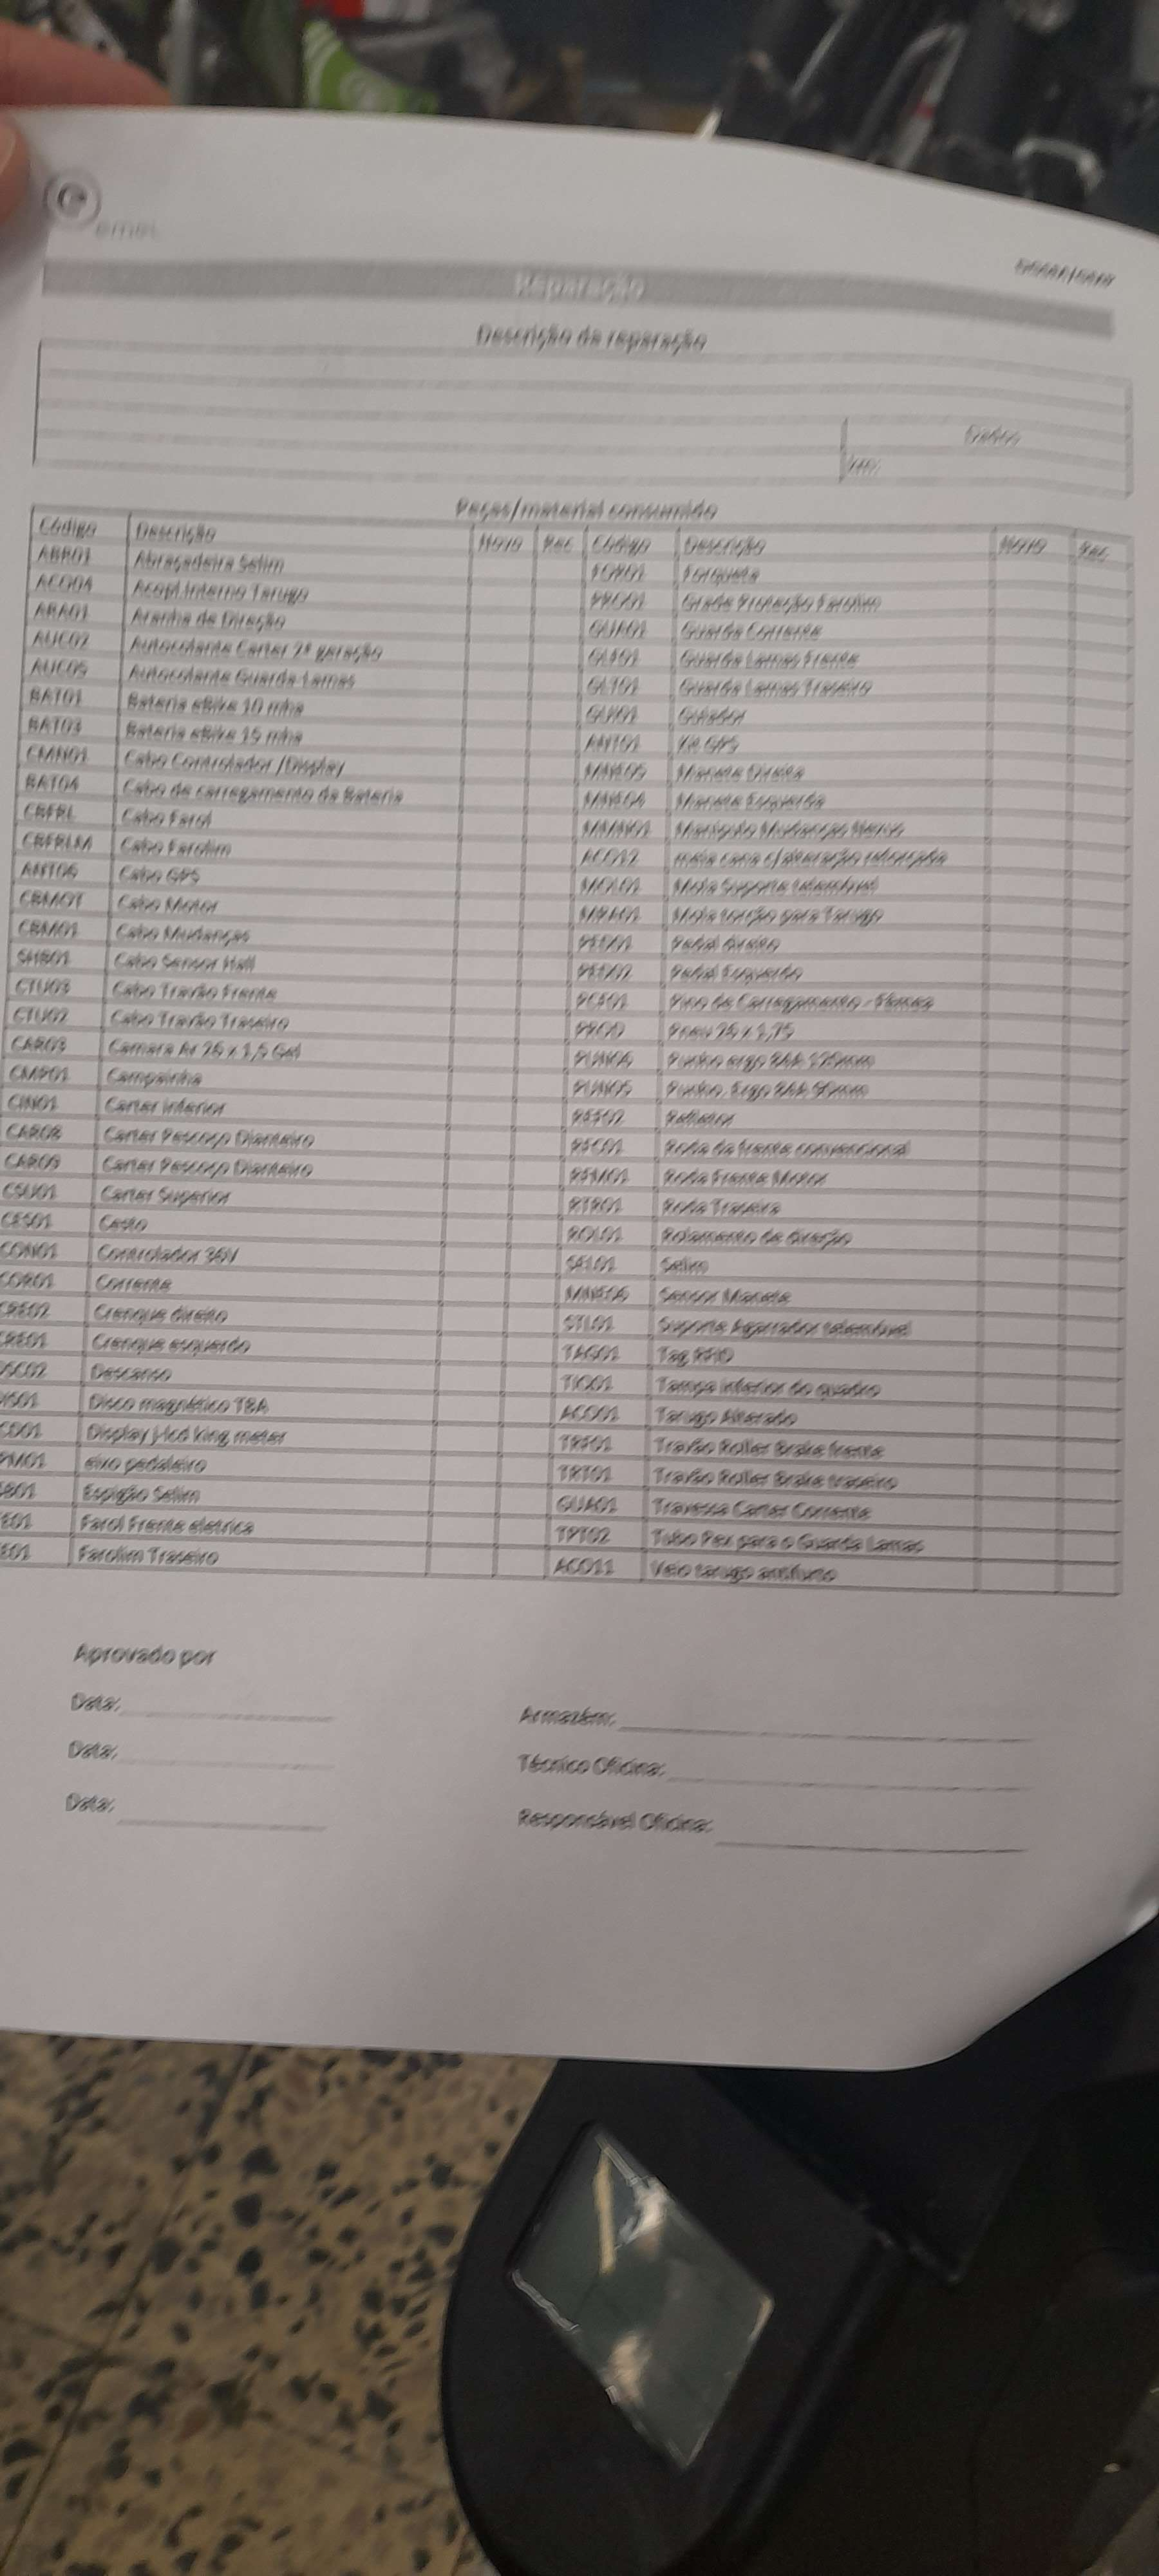
\includegraphics[width=0.50\textwidth]{figs/chapter2/emel_back}
  \label{fig:emel_back}
\end{figure}


\begin{figure}[htbp]
  \caption{\ac{servqual} statements used by the authors in the study to measure the quality of the service at a CMV SA dealership in South Africa (~\cite{Measuring_After_sales_Service_Quality}).}
  \centering
  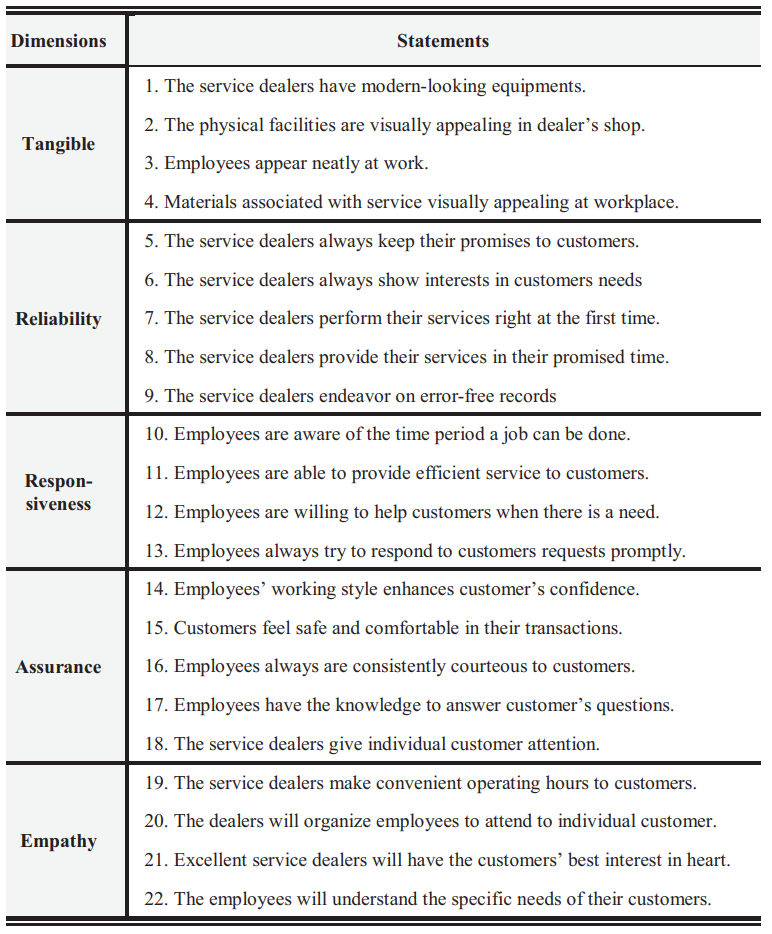
\includegraphics[width=0.75\textwidth]{figs/SERVQUAL_statements}
  \label{fig:SERVQUAL_statements}
\end{figure}


\begin{figure}[htbp]
  \caption{\ac{servqual} results of the study to measure the quality of the service at a CMV SA dealership in South Africa. In the table the header "Exp" means the expectation, "Per" means the perception, "Zc" means the Service quality score from the customers and the "Zc-ms" means Service quality score measure by the difference of the expectations of the customer and the expectation of the dealers. (~\cite{Measuring_After_sales_Service_Quality})}
  \centering
  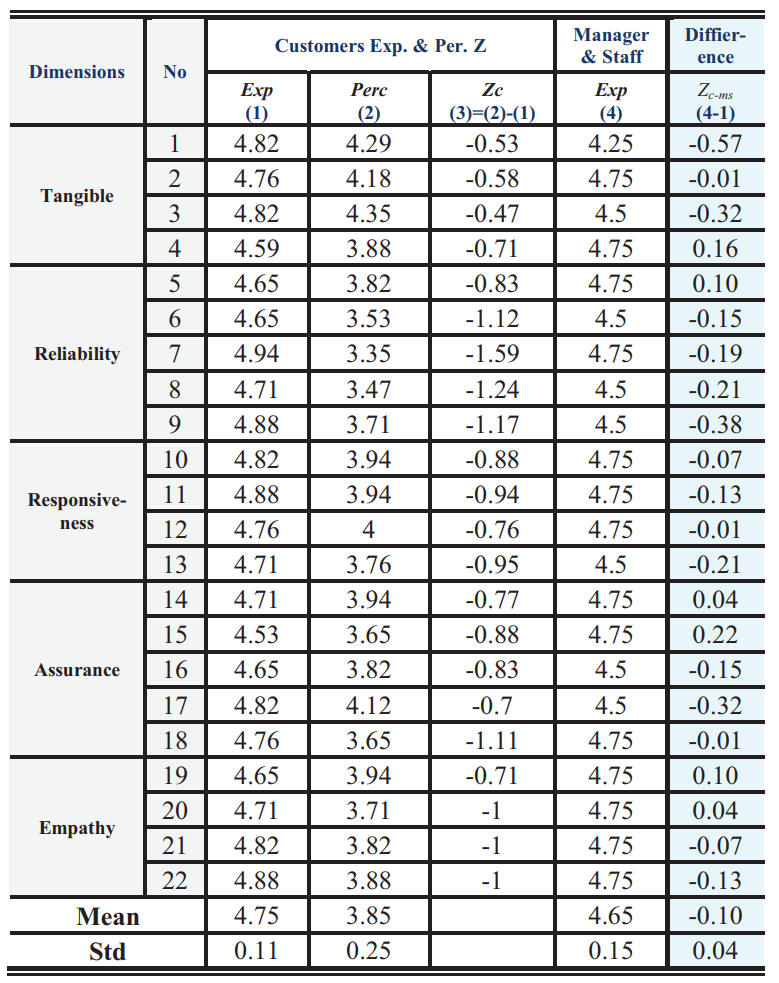
\includegraphics[width=0.75\textwidth]{figs/SERVQUAL_results}
  \label{fig:SERVQUAL_results}
\end{figure}

\begin{table}[ht]
\centering
\resizebox{0.90\textwidth}{!}{%
\begin{tabular}{p{2.5cm} p{6cm} p{6cm} p{1.5cm}}
\hline
\textbf{Dimension} & \textbf{Expectation Survey} & \textbf{Perception Survey} & \textbf{Gap} \\
\hline 
Tangibility & E1. Excellent companies will have modern-looking equipment. & P1. XYZ company has modern-looking equipment. & E - P \\
 & E2. The physical facilities at excellent companies will be visually appealing. & P2. XYZ company’s physical facilities are visually appealing. & \\
 & E3. Employees of excellent companies will be neat-appearing. & P3. XYZ company’s employees are neat-appearing. & \\
 & E4. Materials associated with the service (such as pamphlets or statements) will be visually appealing in excellent companies. & P4. Materials associated with the service (such as pamphlets or statements) are visually appealing at XYZ company. & \\
\hline
Reliability & E5. When excellent companies promise to do something by a certain time, they do so. & P5. When XYZ company promises to do something by a certain time, it does so. & \\
 & E6. When customers have a problem, excellent companies will show sincere interest in solving it. & P6. When you have a problem, XYZ company shows a sincere interest in solving it. & \\
 & E7. Excellent companies will perform the service right the first time. & P7. XYZ company performs the service right the first time. & \\
 & E8. Excellent companies will provide the services at the time they promise to do so. & P8. XYZ company provides its services at the time it promises to do so. & \\
 & E9. Excellent companies will insist on error-free records. & P9. XYZ company insists on error-free records. & \\
\hline
Responsiveness & E10. Employees of excellent companies will tell customers exactly when services will be performed. & P10. Employees of XYZ company tell you exactly when services will be performed. & \\
 & E11. Employees of excellent companies will provide prompt services to customers. & P11. Employees of XYZ company give you prompt service. & \\
 & E12. Employees of excellent companies will always be willing to help customers. & P12. Employees of XYZ company are always willing to help you. & \\
 & E13. Employees of excellent companies will never be too busy to respond to customers. & P13. Employees of XYZ company are never too busy to respond to your requests. & \\
\hline
Assurance & E14. The behavior of employees at excellent companies will instill confidence in customers. & P14. The behavior of employees of XYZ company instills confidence in customers. & \\
 & E15. Customers of excellent companies will feel safe in their transactions. & P15. You feel safe in your transactions with XYZ company. & \\
 & E16. Employees of excellent companies will be consistently courteous with customers. & P16. Employees of XYZ company are consistently courteous with you. & \\
 & E17. Employees of excellent companies will have the knowledge to answer customers’ questions. & P17. Employees of XYZ company have the knowledge to answer your questions. & \\
\hline
Empathy & E18. Excellent companies will give customers individual attention. & P18. XYZ company gives you individual attention. & \\
 & E19. Excellent companies will have operating hours convenient to all their customers. & P19. XYZ company has operating hours convenient to all its customers. & \\
 & E20. Excellent companies will have employees who give customers personal attention. & P20. XYZ company has employees who give you personal attention. & \\
 & E21. Excellent companies will have customer’s best interests at heart. & P21. XYZ company has your best interests at heart. & \\
 & E22. The employees of excellent companies will understand the specific needs of their customers. & P22. Employees of XYZ company understand your specific needs. & \\
\hline
\end{tabular}
}
\caption{\ac{servqual} Questionnaire Template (Expectations vs Perceptions) ~\cite{master_servqual_model}} 
\label{table:servqual_template}
\end{table}



\foreach \p in {1,...,4}{%  <-- change 5 to the total number of pages
\begin{figure}[p]
  \caption{Database indexes— page \p}
  \centering
  \includegraphics[page=\p,width=\textwidth]{figs/dbDiagrams/BD_indexes}
  \label{fig:BD_indexes-\p}
\end{figure}
}



\begin{figure}[htbp]
  \caption{Active maintenance details Information tab.}
  \centering
  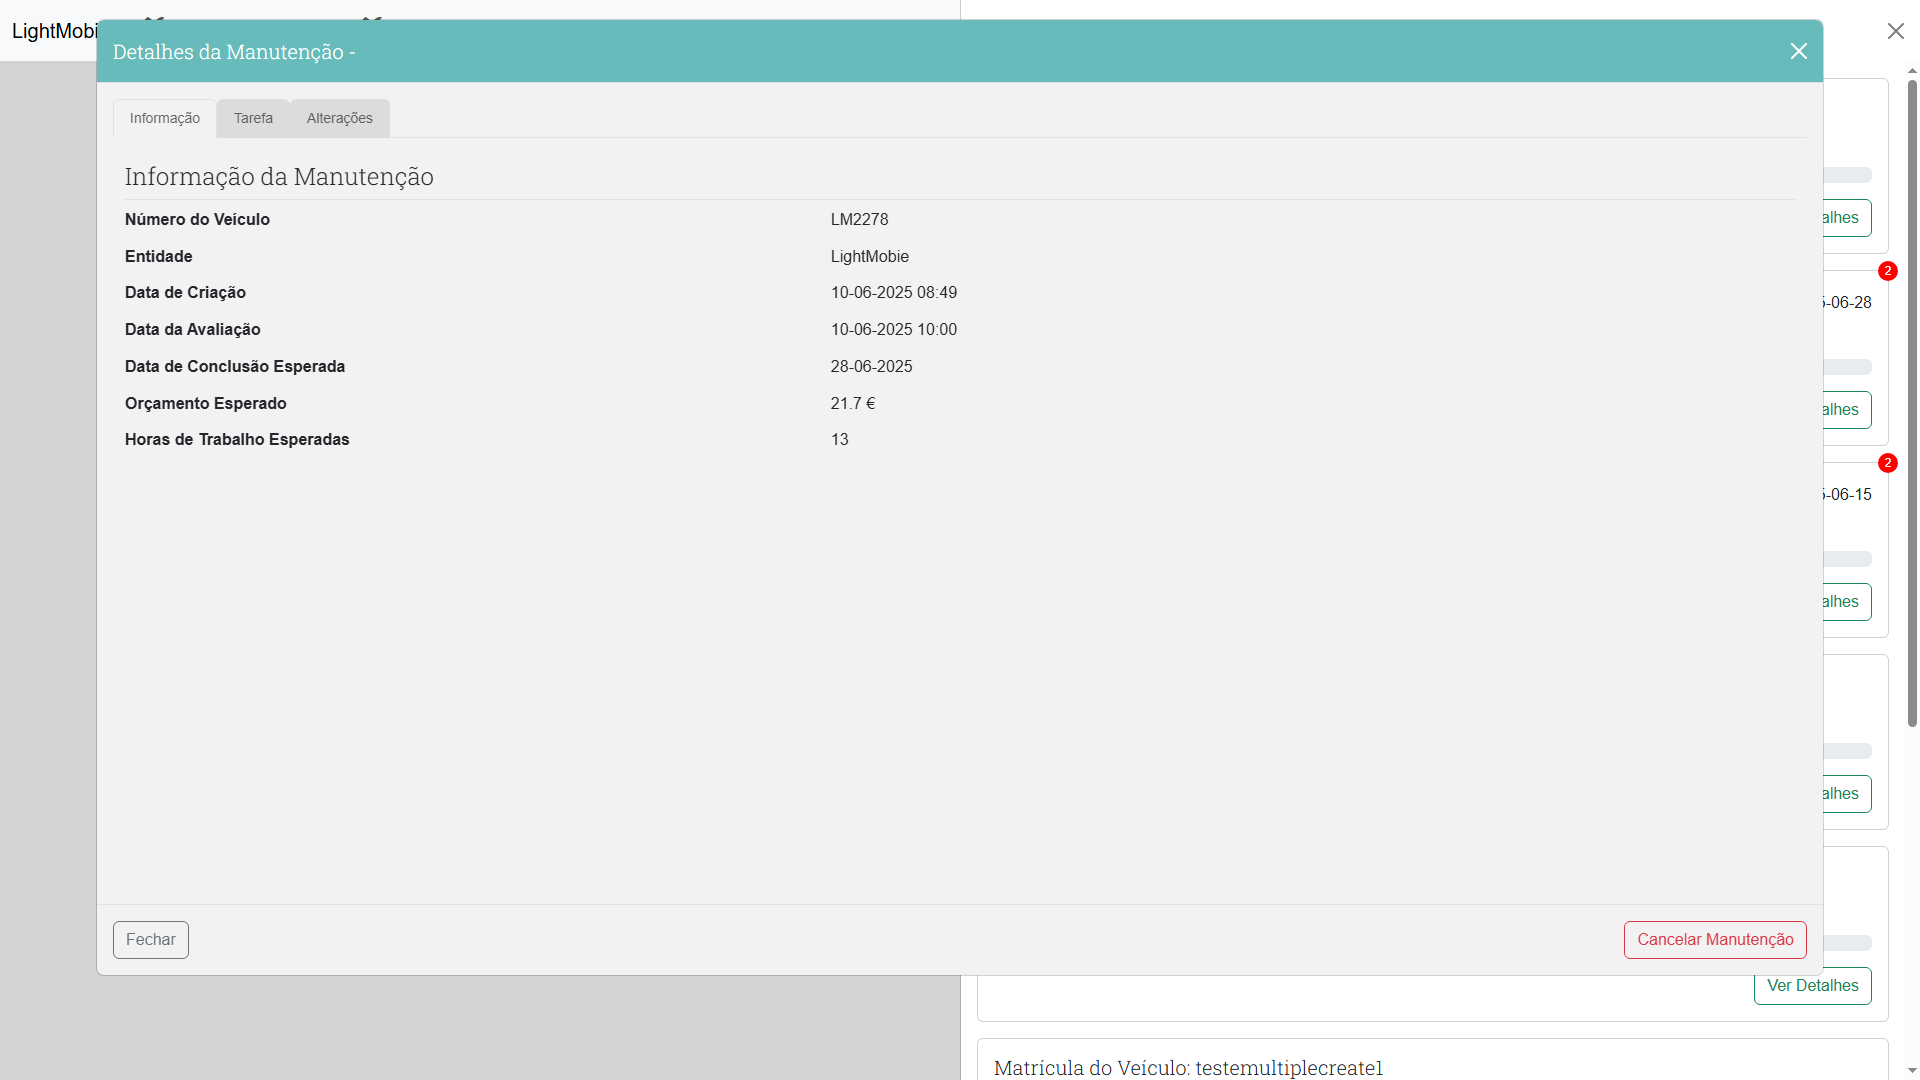
\includegraphics[width=\textwidth]{figs/Implementation/rececionist/maintenance_details}
  \label{fig:impReceMaintHome}
\end{figure}




\begin{figure}[htbp]
  \caption{Example of the confirmation email sent to the client. The layout used for dealership employees is similar.}
  \centering
  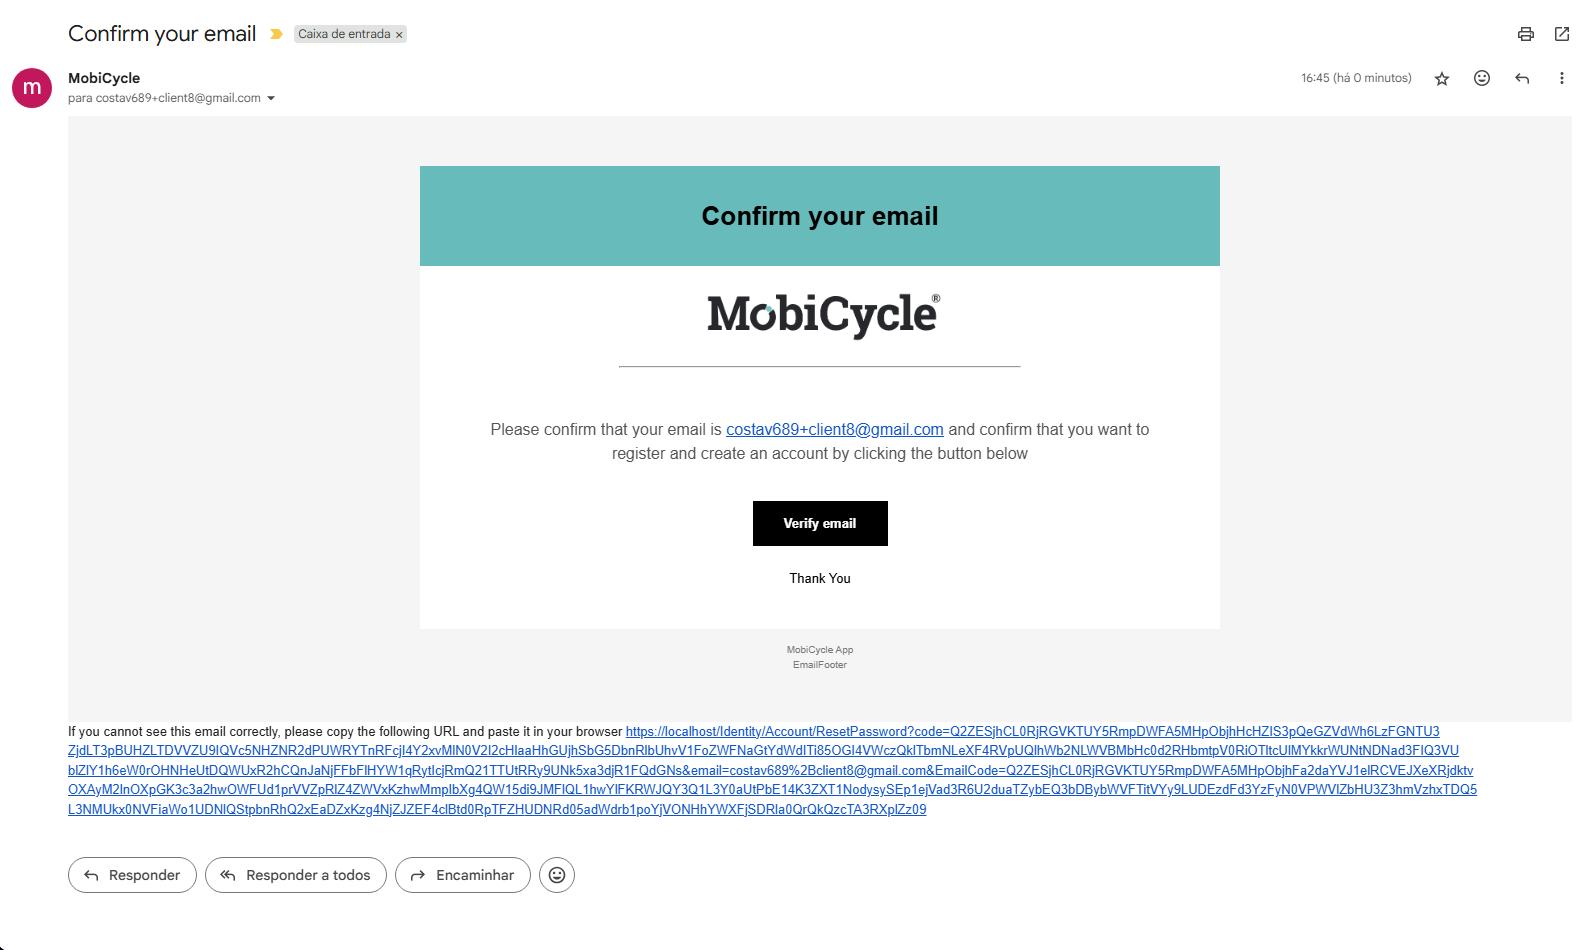
\includegraphics[width=\textwidth]{figs/Implementation/rececionist/CreateClient}
  \label{fig:CreateClient}
\end{figure}



\begin{figure}[htbp]
  \caption{Form where the client fills in the remaining required personal information.}
  \centering
  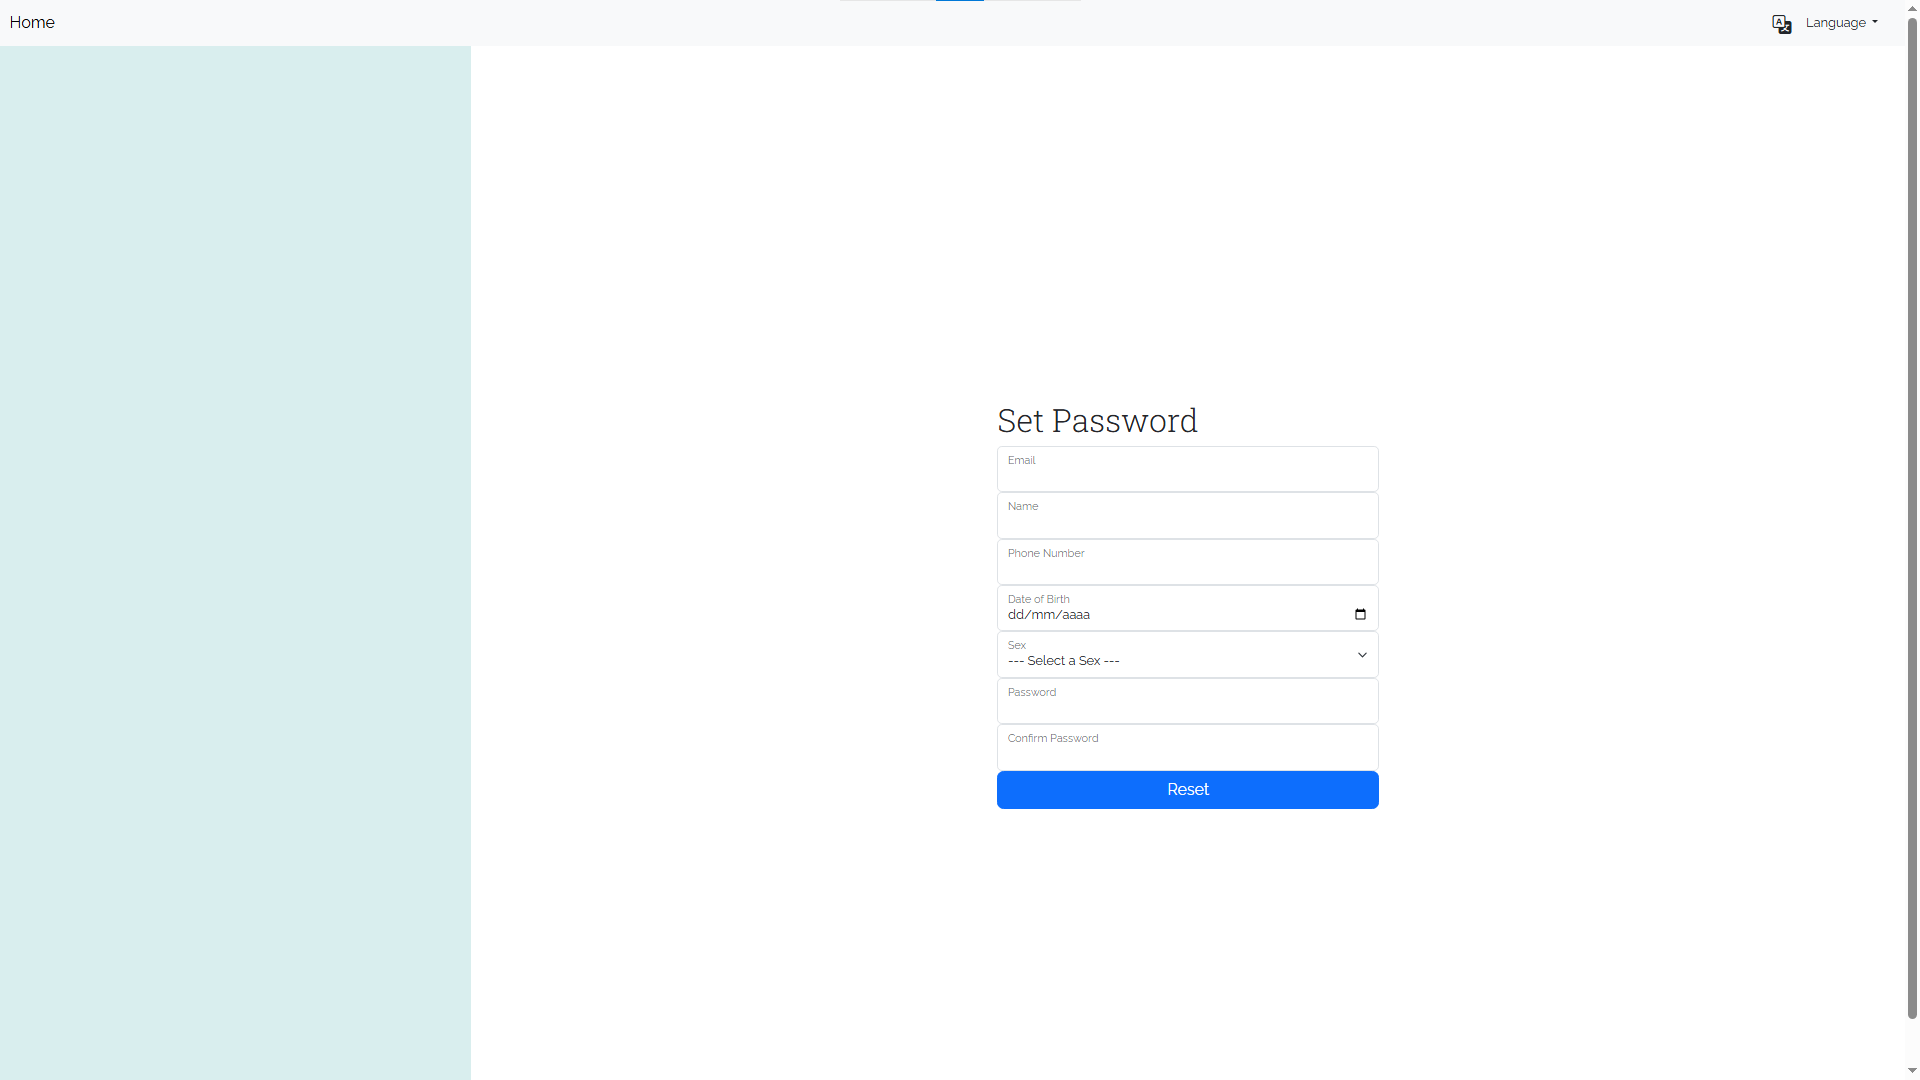
\includegraphics[width=\textwidth]{figs/Implementation/rececionist/SetPassword}
  \label{fig:SetPassword}
\end{figure}

\begin{figure}[htbp]
  \caption{Active maintenance details task tab.}
  \centering
  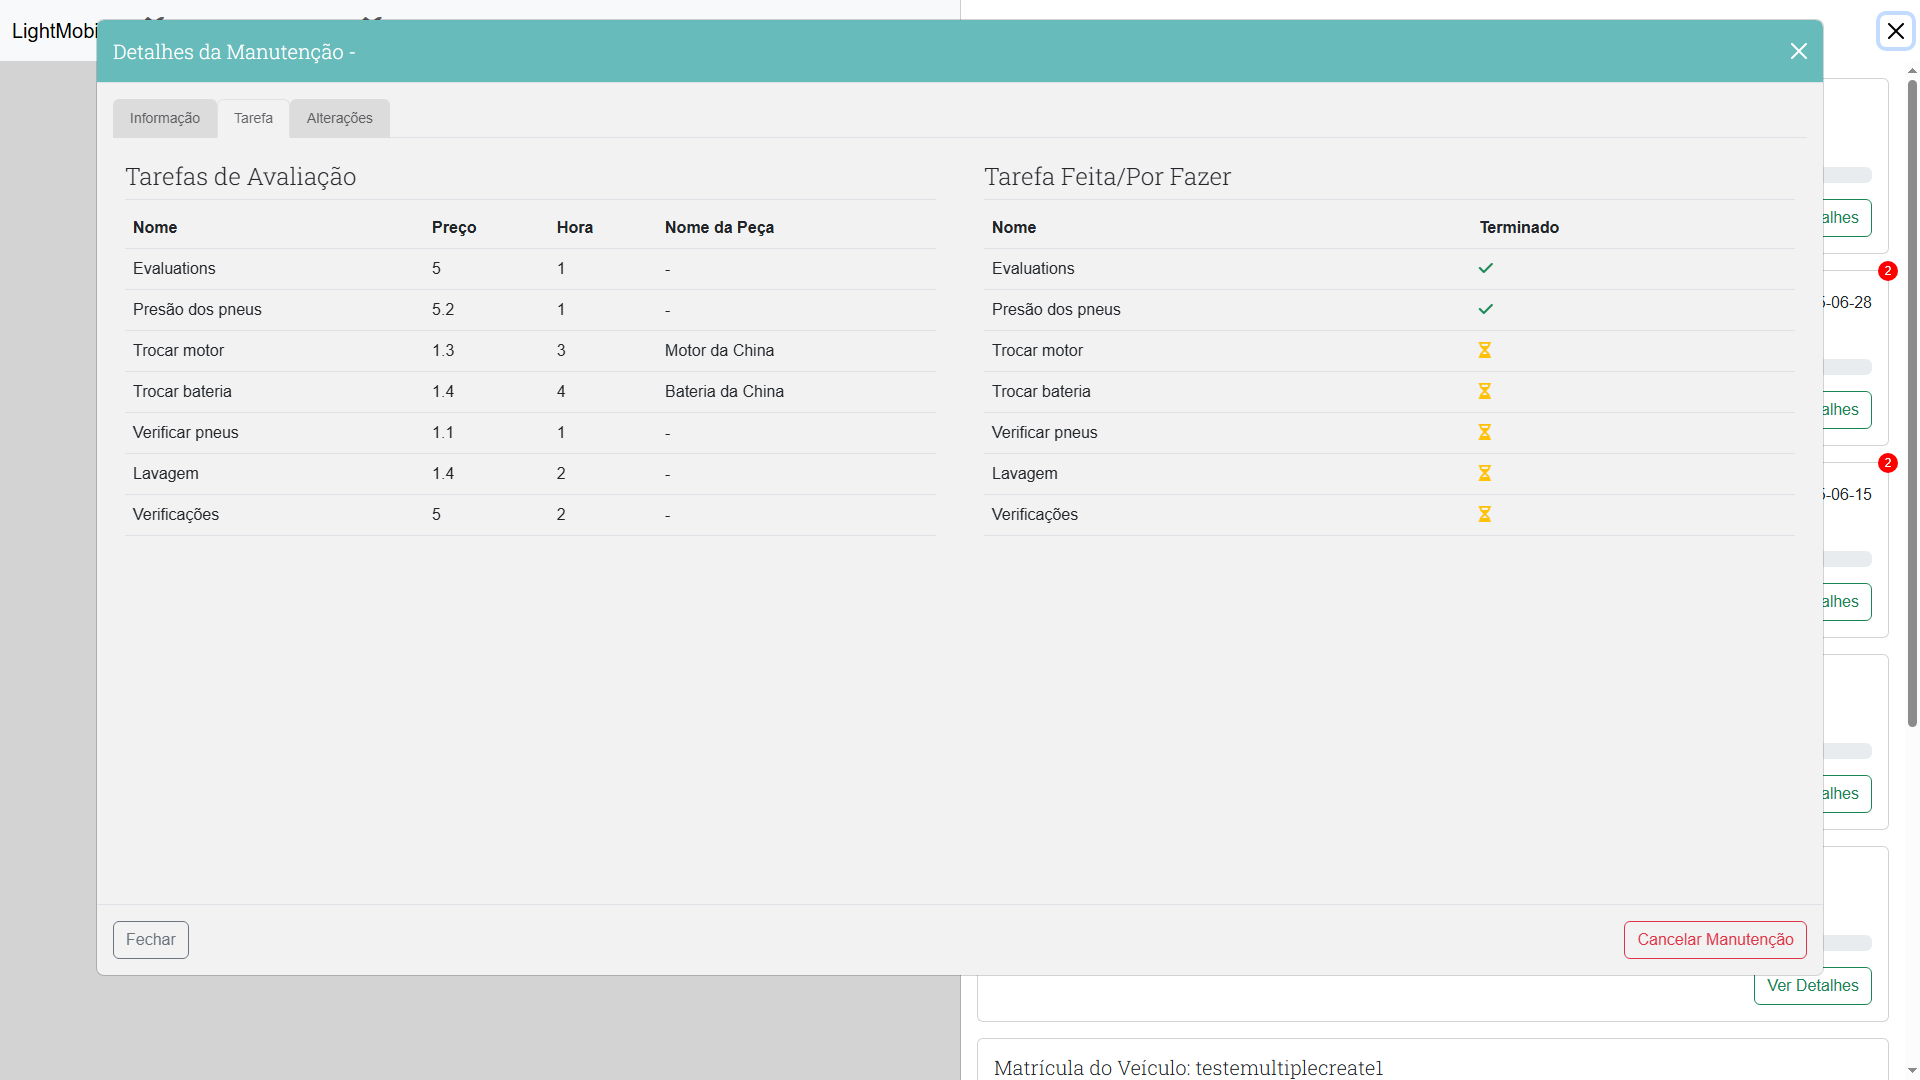
\includegraphics[width=\textwidth]{figs/Implementation/rececionist/maintenance_details_task}
  \label{fig:impReceMaintTask}
\end{figure}

\begin{figure}[htbp]
  \caption{Active maintenance details change tab.}
  \centering
  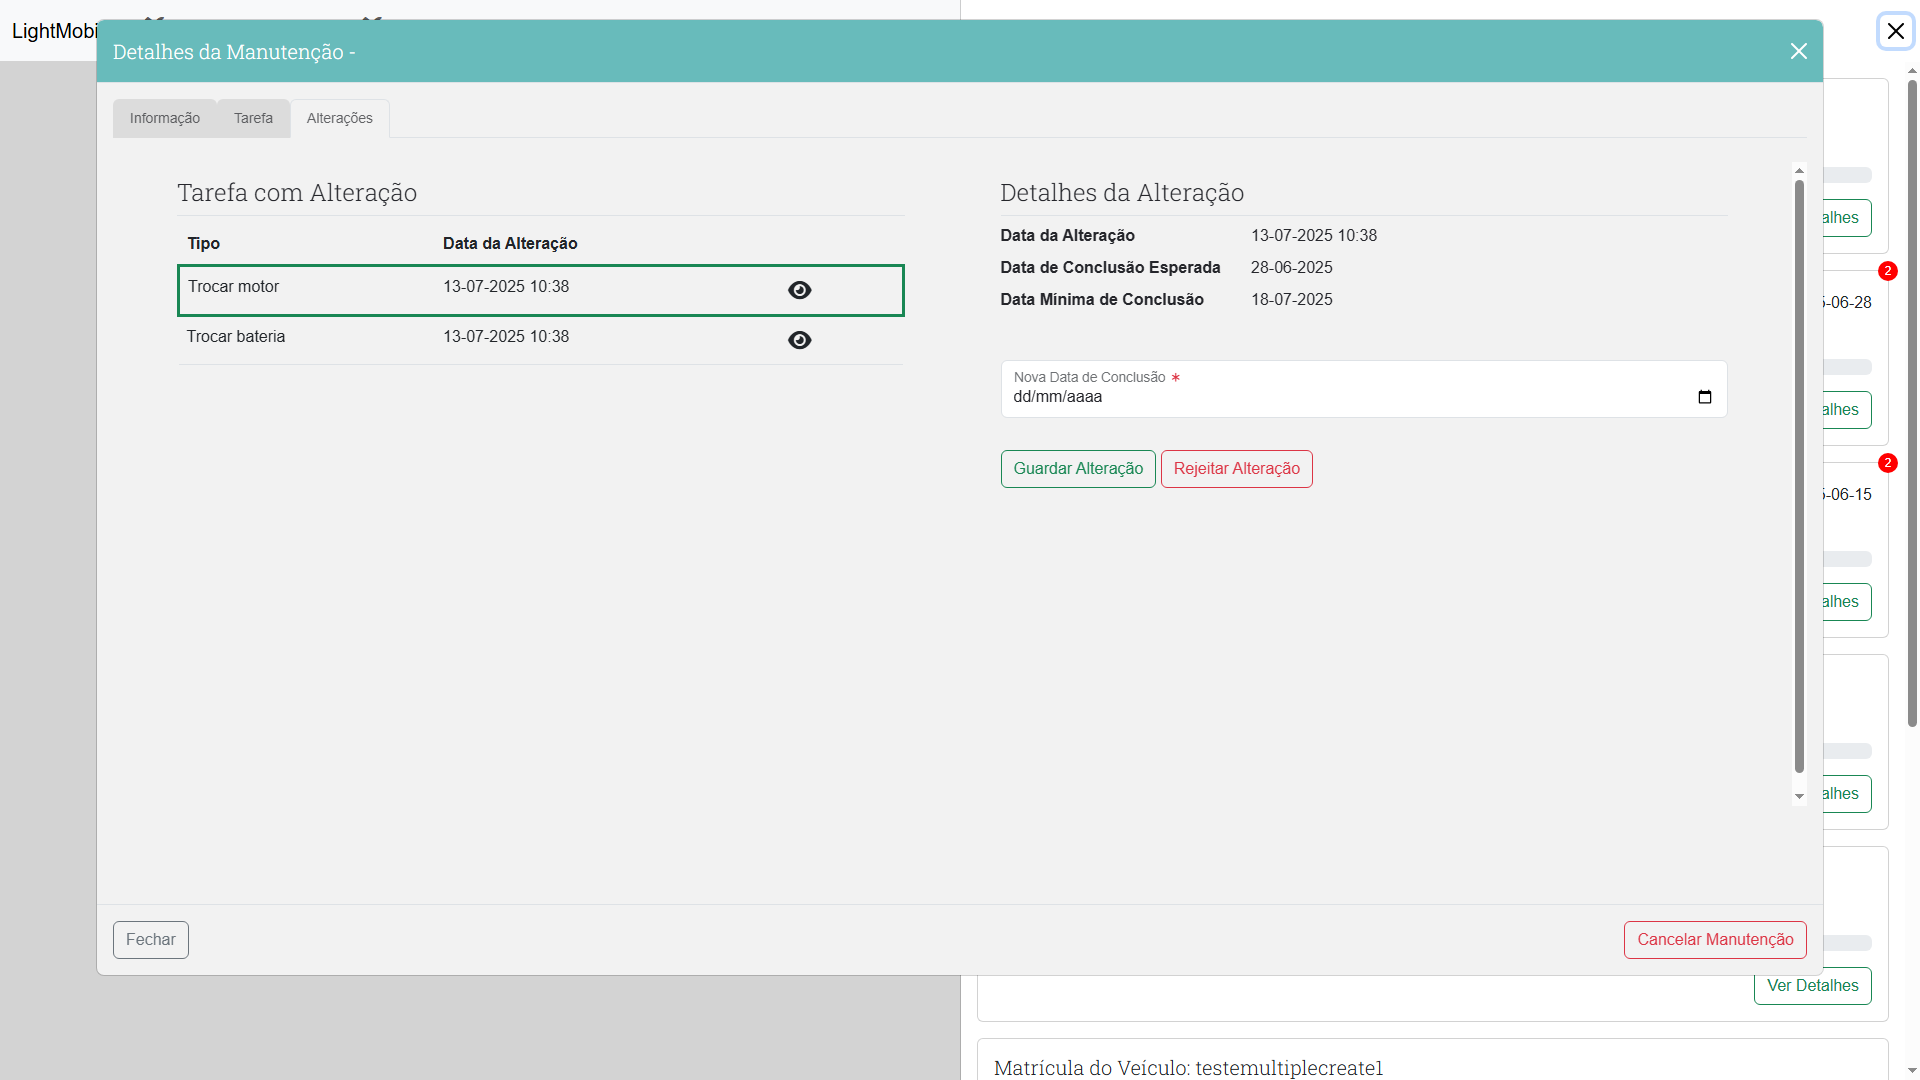
\includegraphics[width=\textwidth]{figs/Implementation/rececionist/maintenance_details_change}
  \label{fig:impReceMaintChange}
\end{figure}




\begin{figure}[htbp]
  \caption{Mechanic completing simple task first step.}
  \centering
  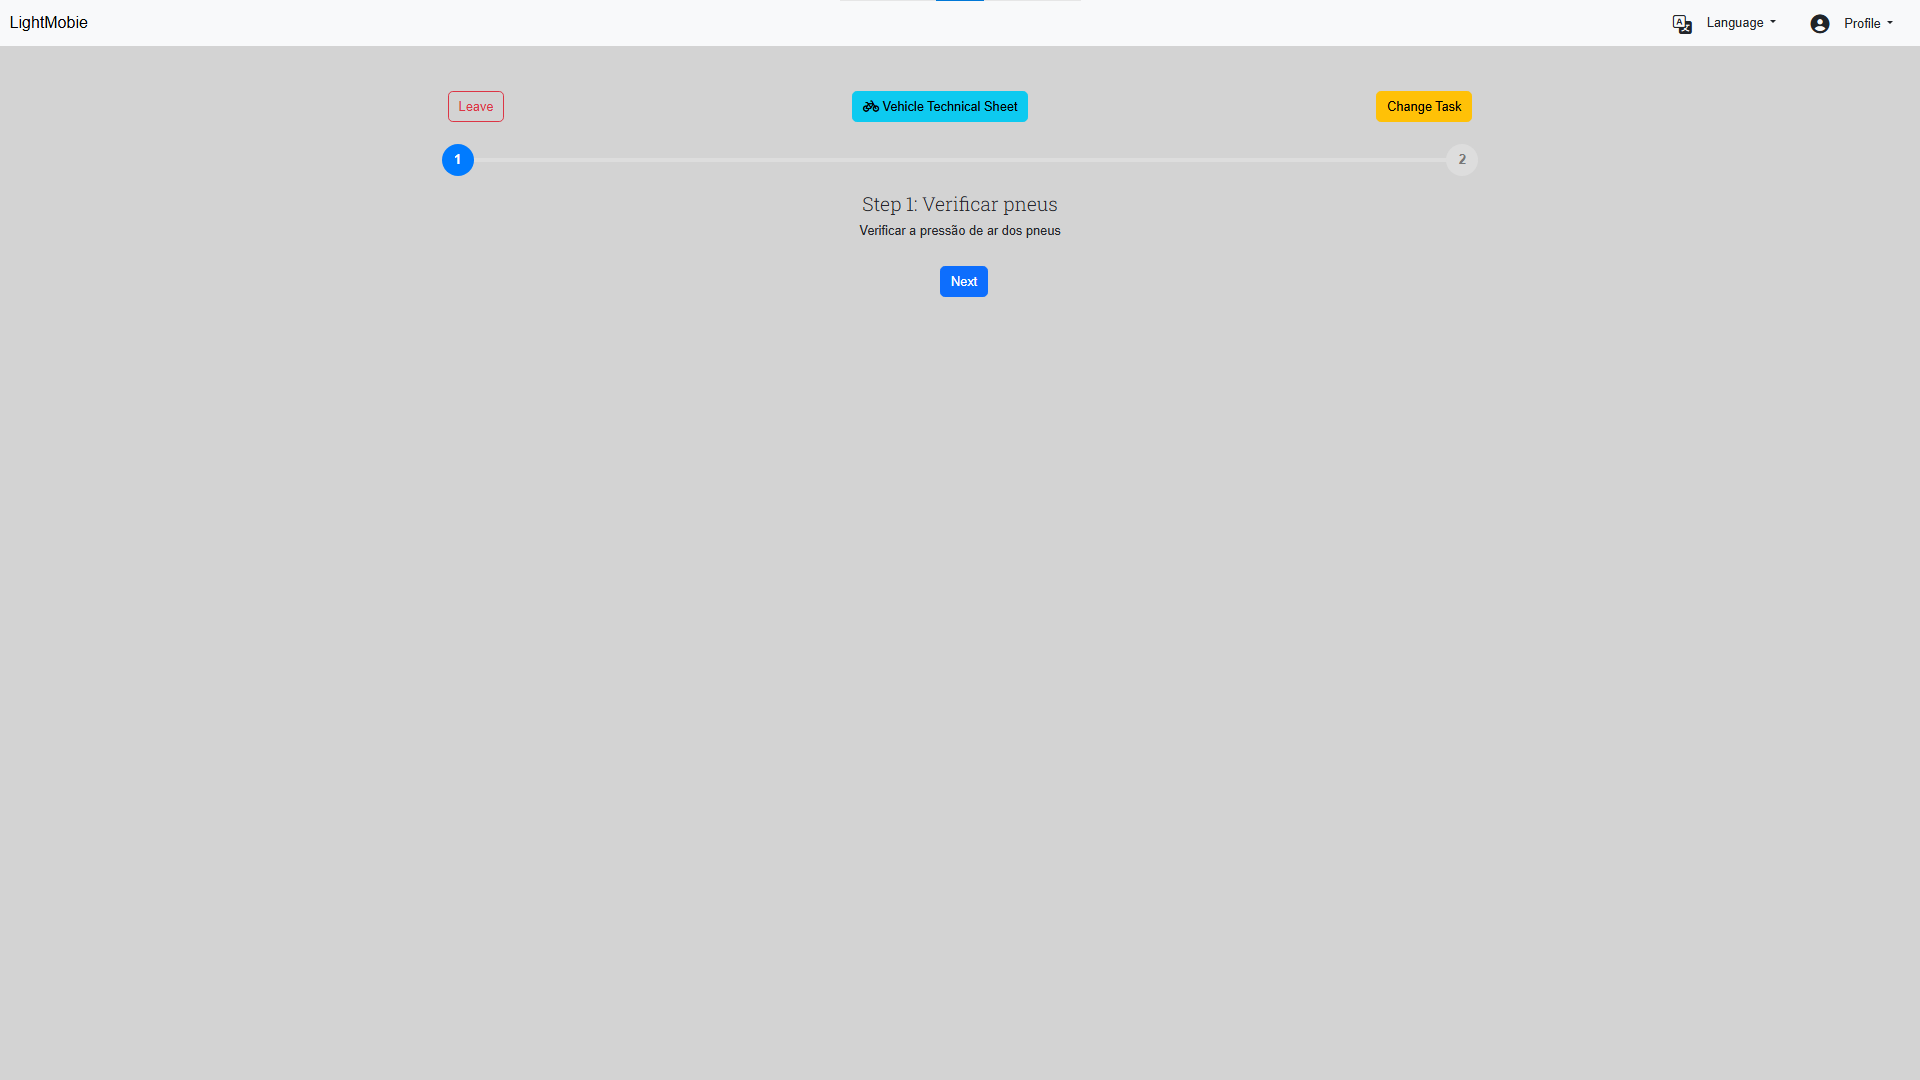
\includegraphics[width=\textwidth]{figs/Implementation/mechanic/MechanicTaskNormal}
  \label{fig:MechanicTaskNormal}
\end{figure}



\begin{figure}[htbp]
  \caption{Change task modal.}
  \centering
  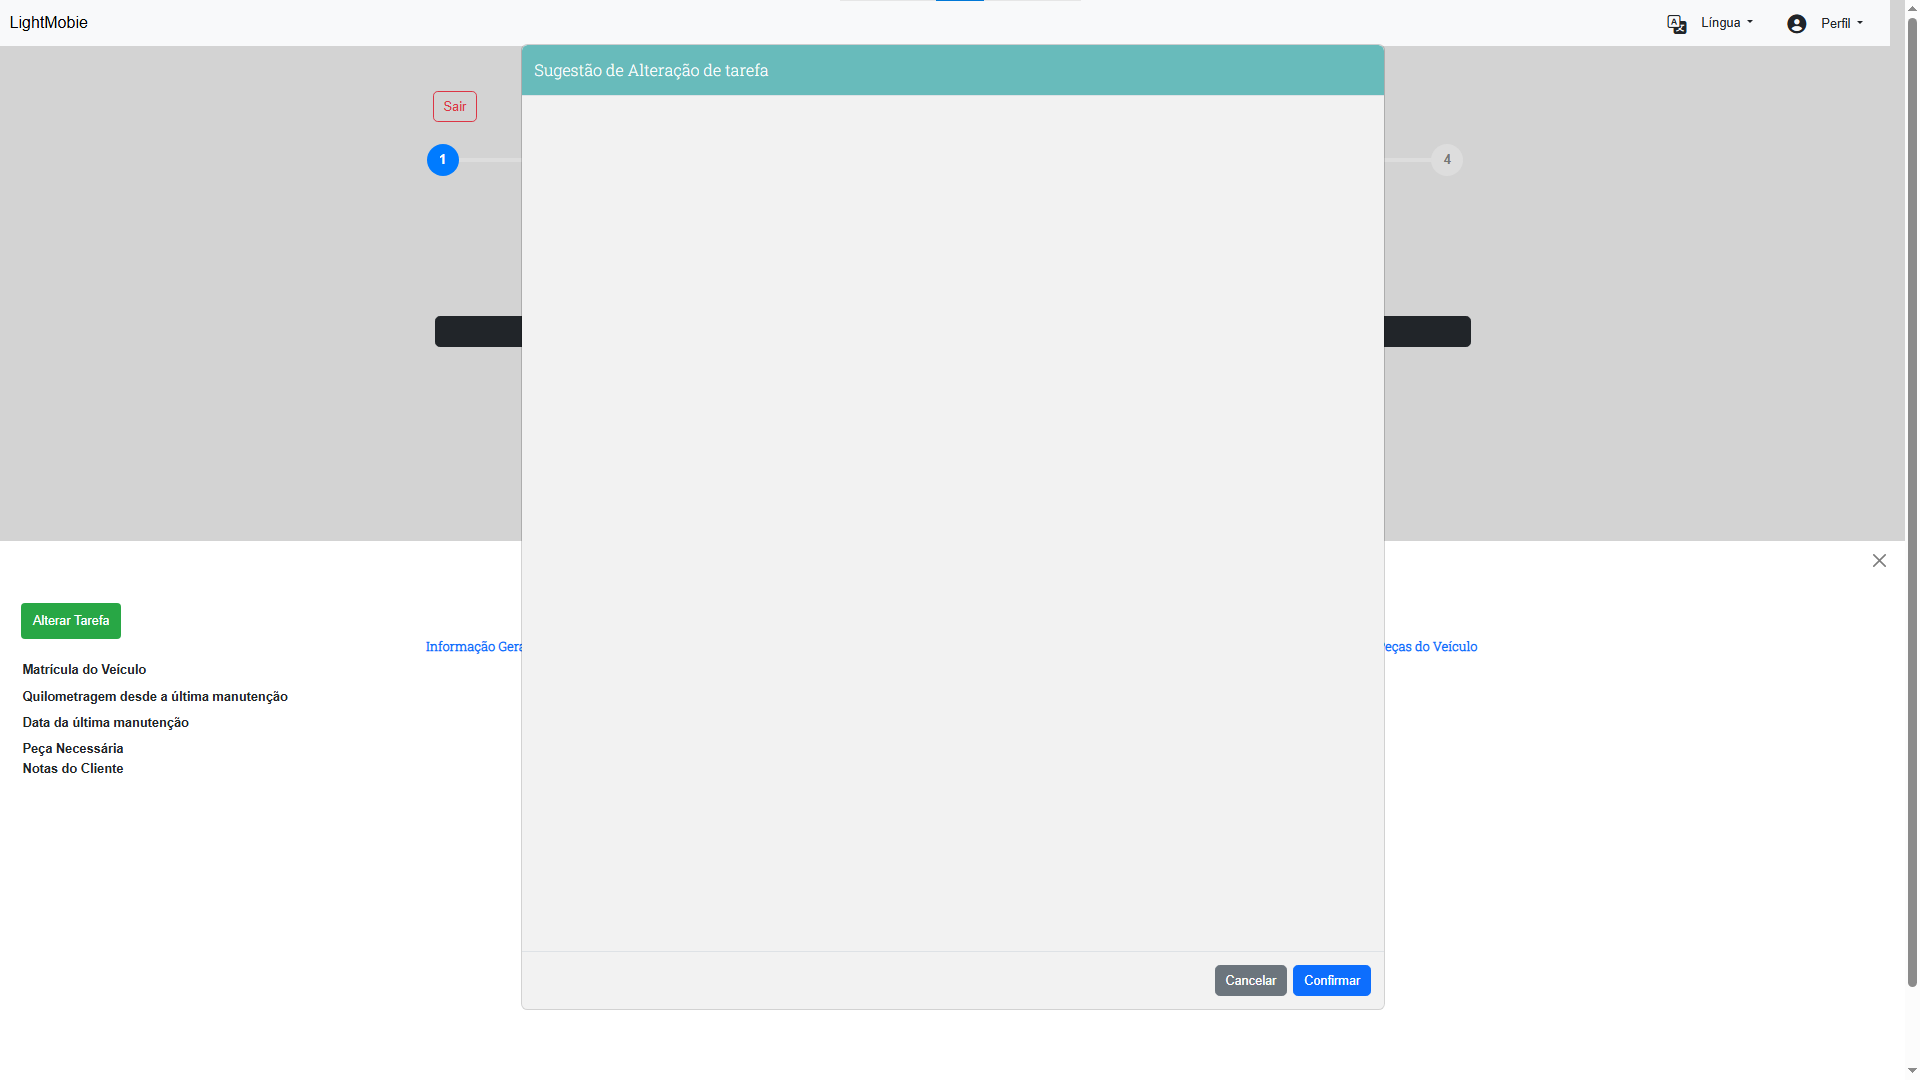
\includegraphics[width=\textwidth]{figs/Implementation/mechanic/MechanicTaskChangeTask}
  \label{fig:MechanicTaskChangeTask}
\end{figure}


\begin{figure}[htbp]
  \caption{Mechanic task last step.}
  \centering
  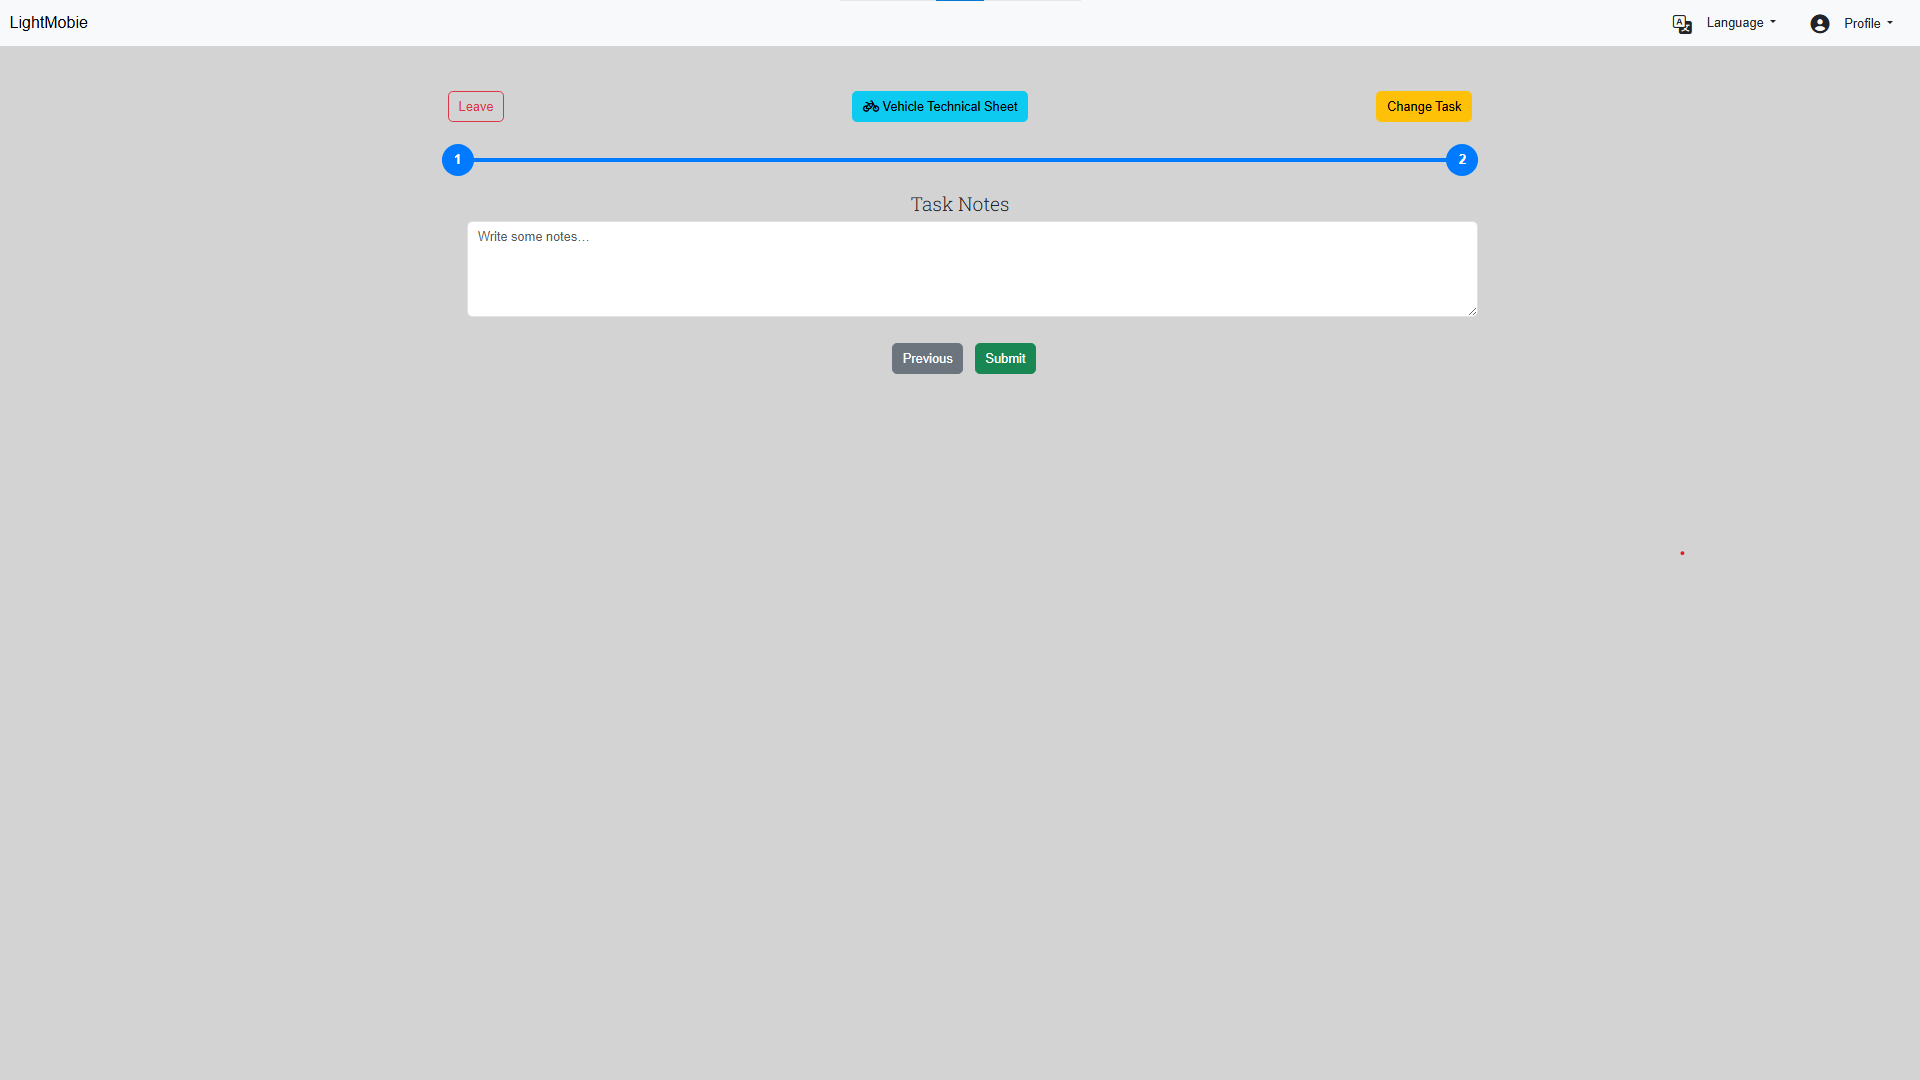
\includegraphics[width=\textwidth]{figs/Implementation/mechanic/MechanicTaskLastStep}
  \label{fig:MechanicTaskLastStep}
\end{figure}




\begin{figure}[htbp]
  \caption{Mechanic select part modal.}
  \centering
  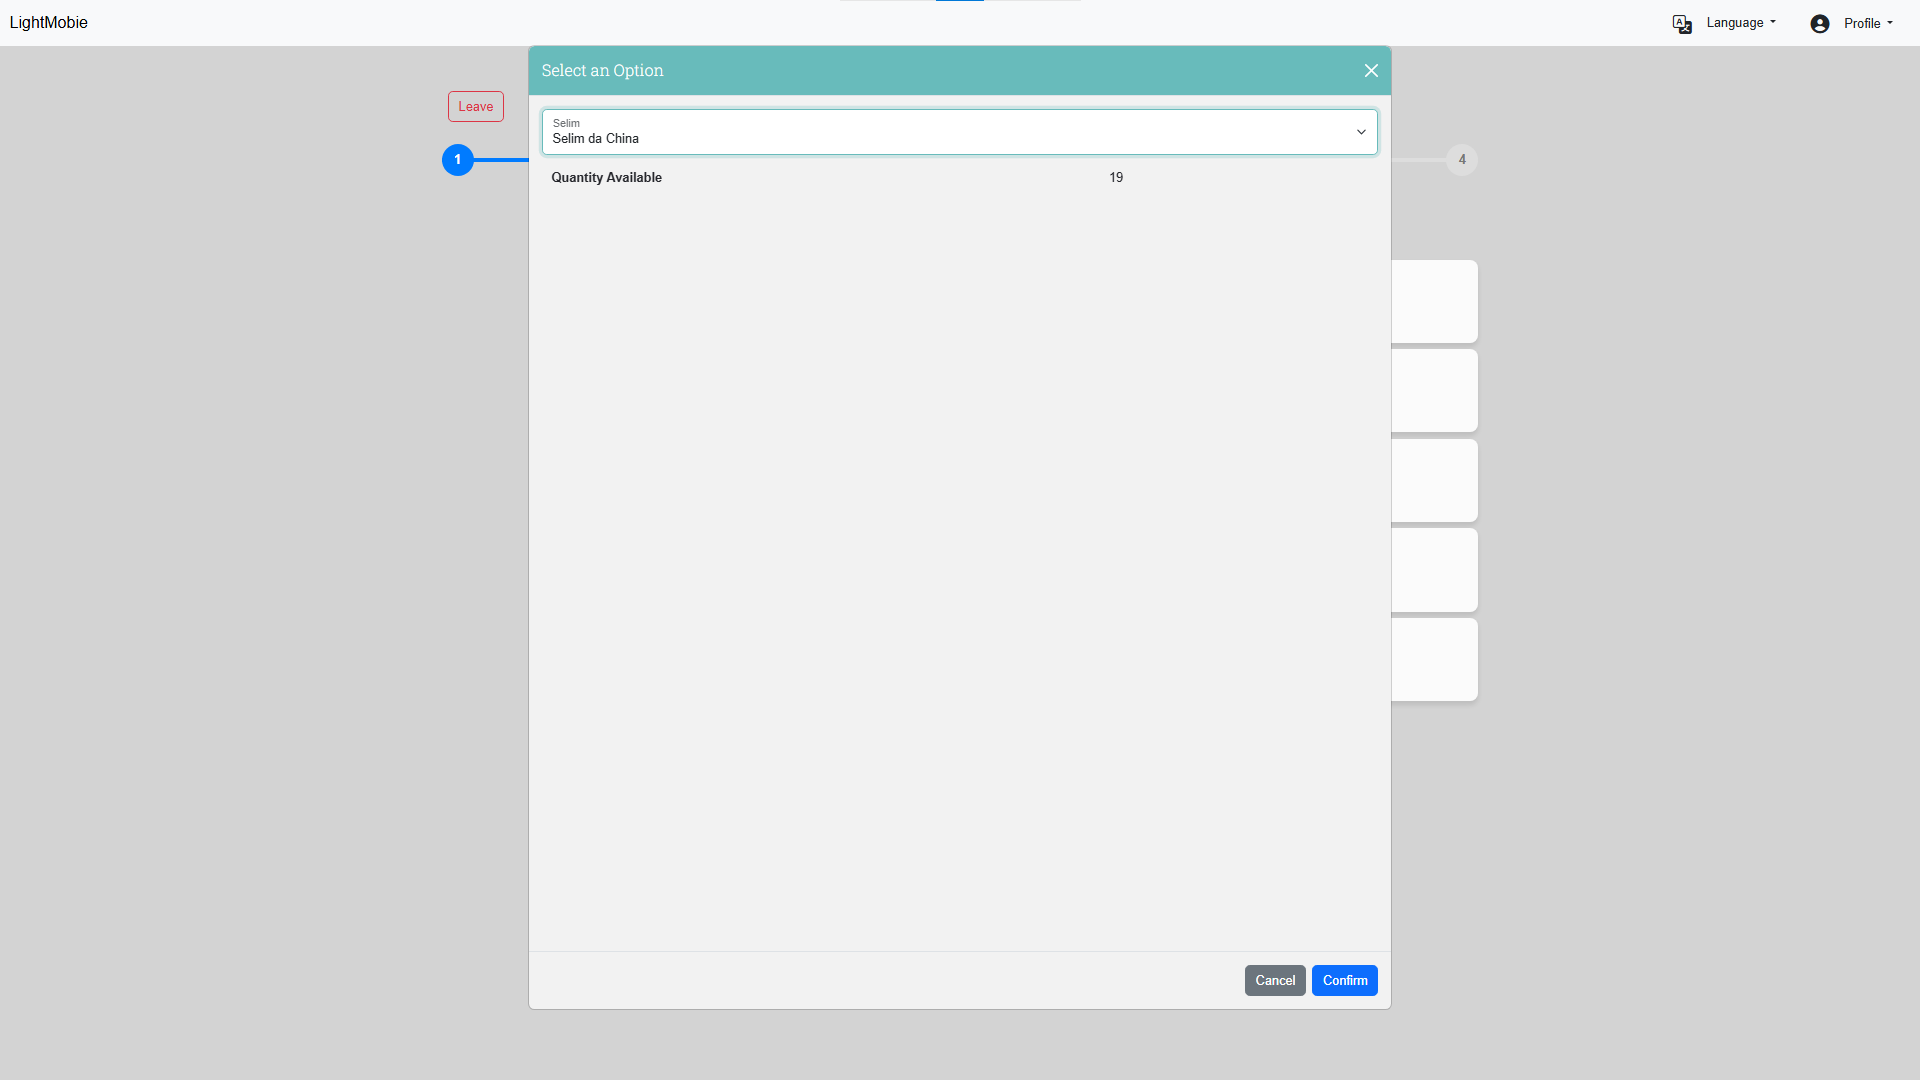
\includegraphics[width=\textwidth]{figs/Implementation/mechanic/MechanicEvaluationSelectTaskWitPart}
  \label{fig:MechanicEvaluationSelectTaskWitPart}
\end{figure}

\begin{figure}[htbp]
  \caption{Mechanic Evaluation task with part selected.}
  \centering
  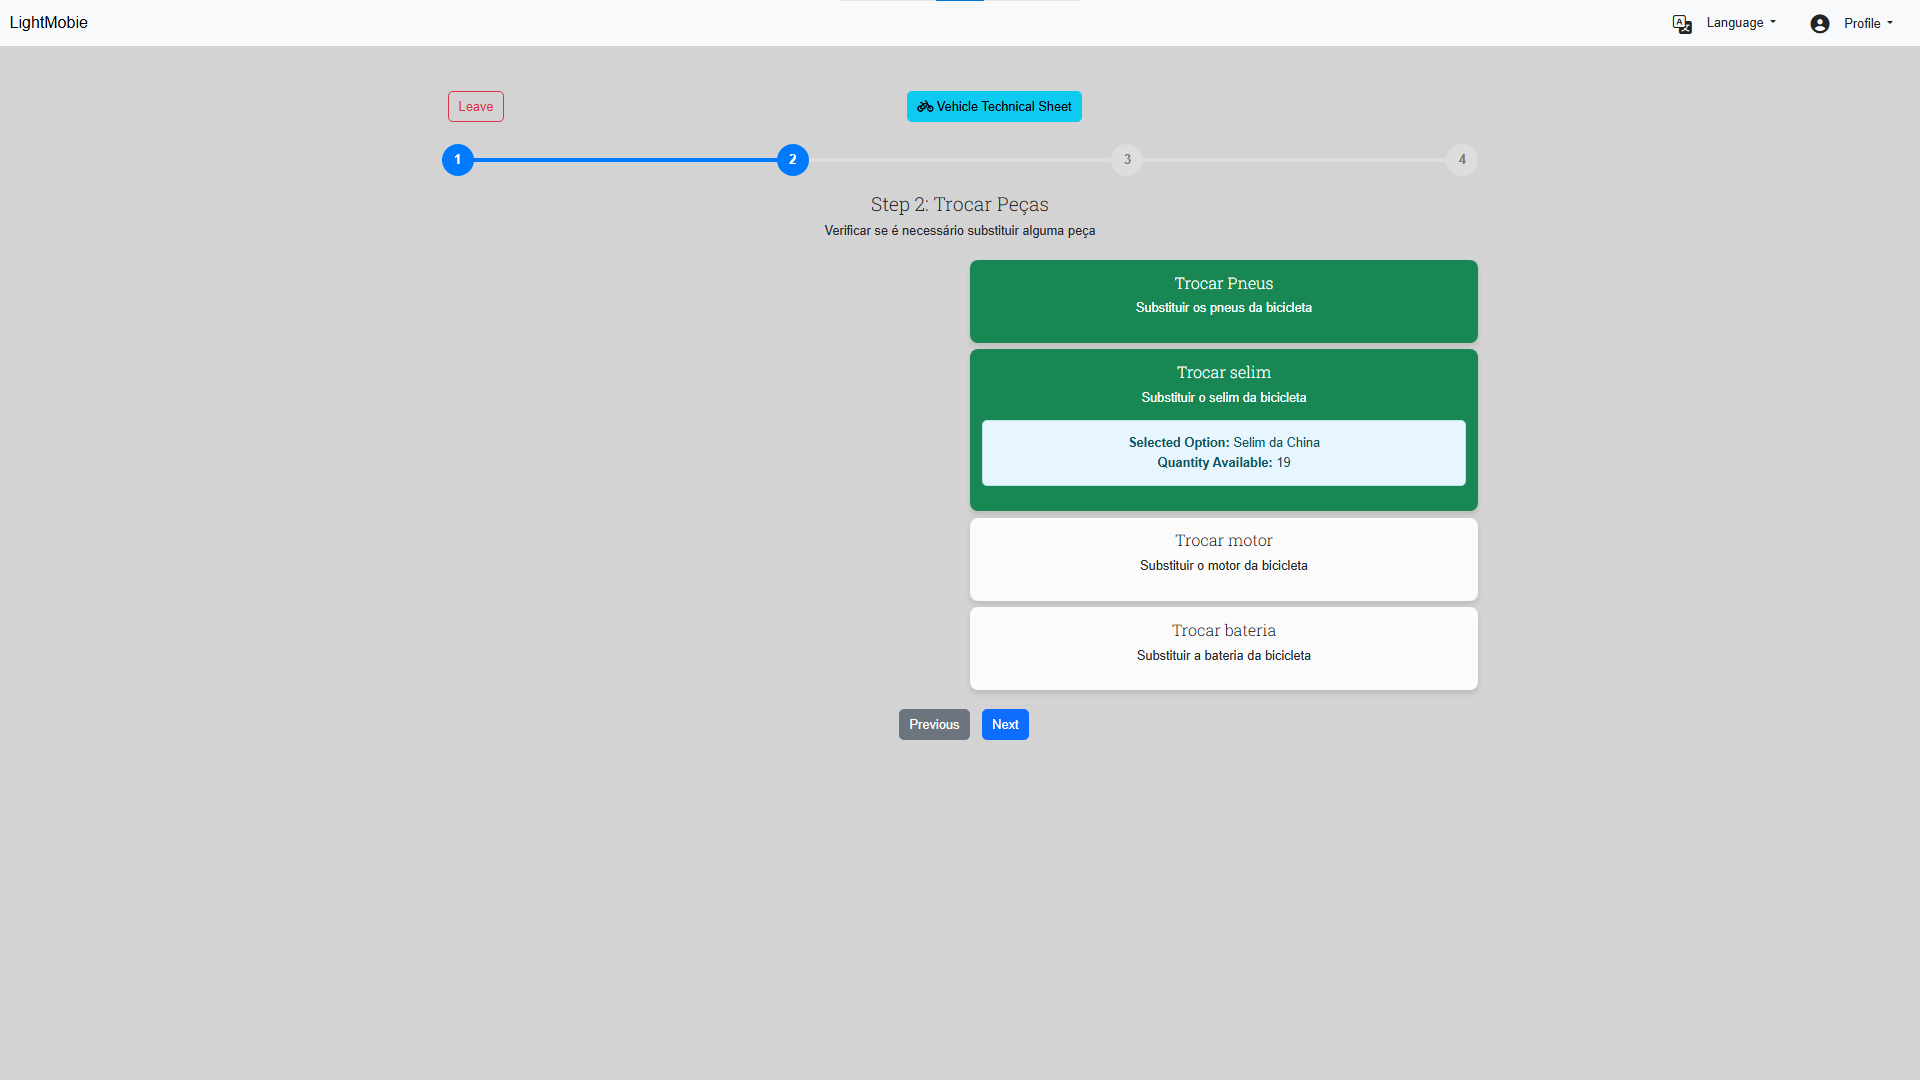
\includegraphics[width=\textwidth]{figs/Implementation/mechanic/TaskSelected}
  \label{fig:TaskSelected}
\end{figure}



\begin{figure}[htbp]
  \caption{Mechanic Evaluation last step.}
  \centering
  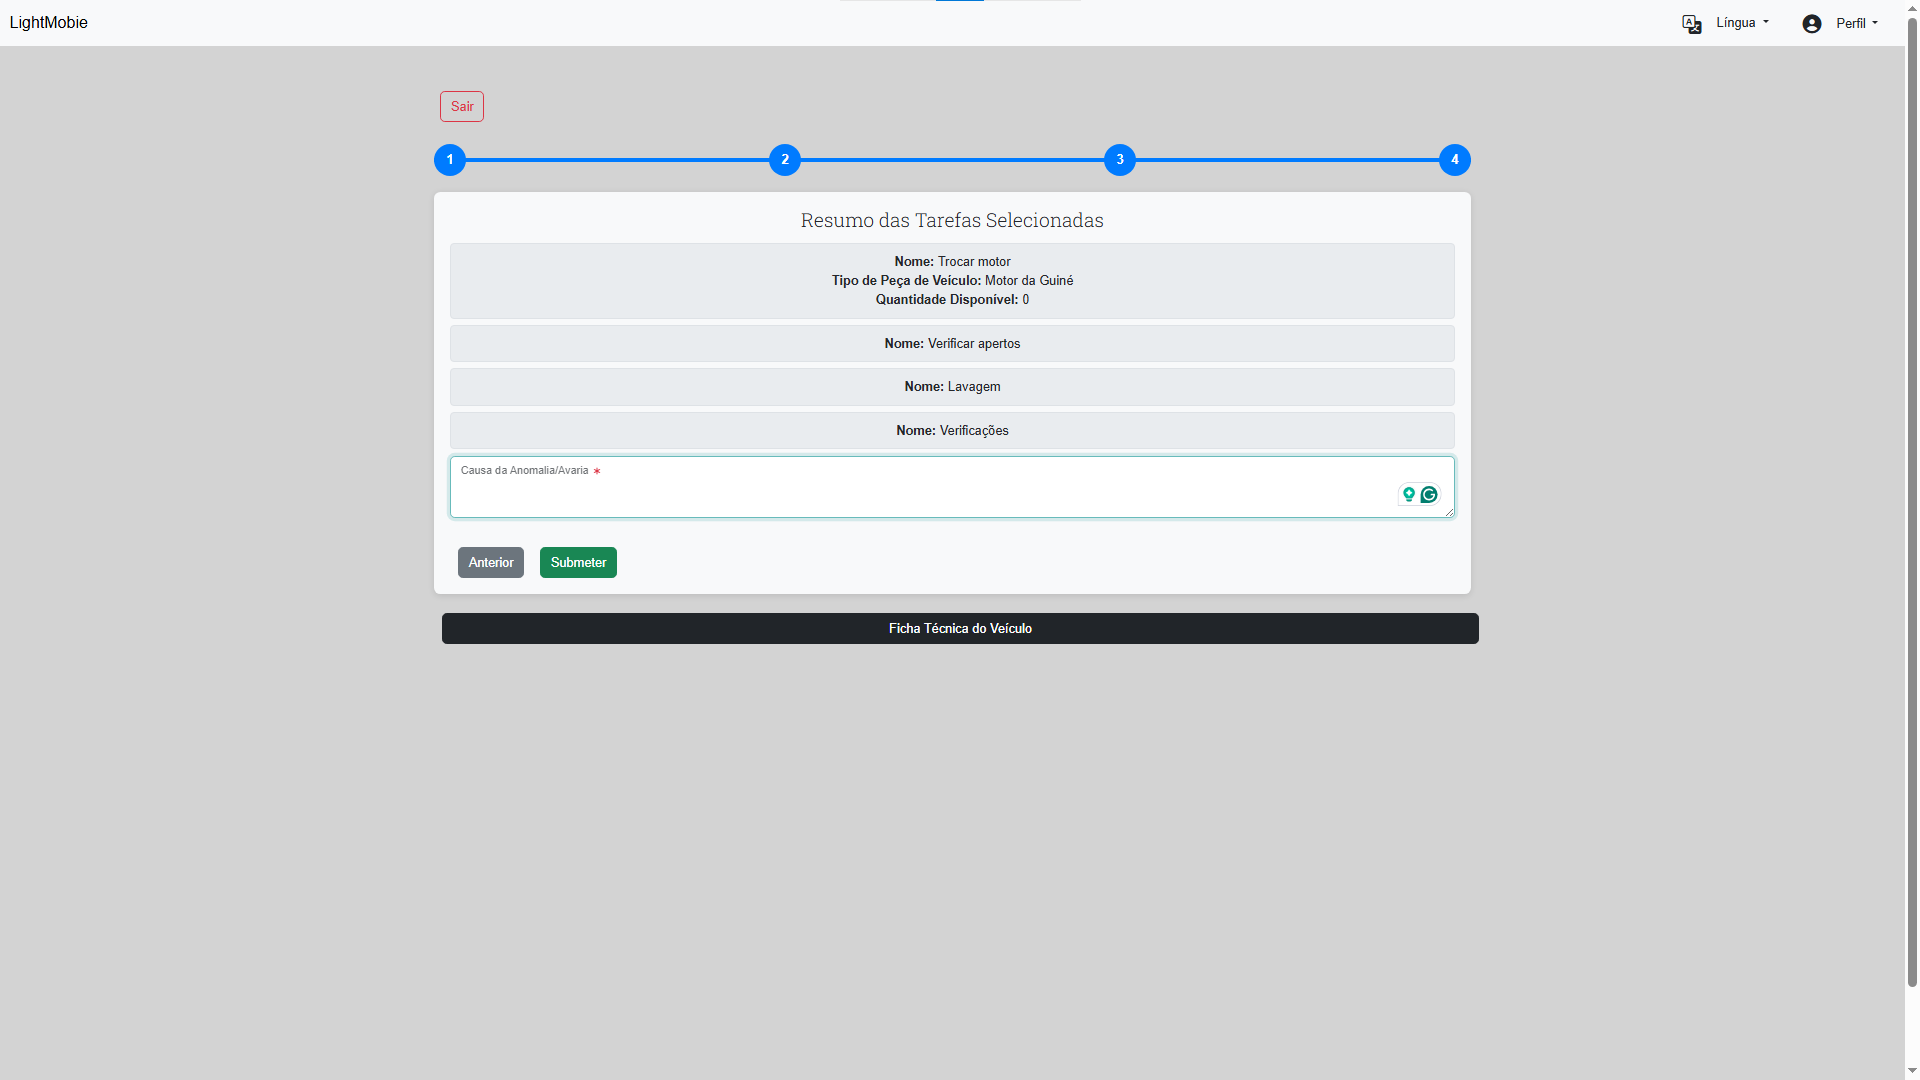
\includegraphics[width=\textwidth]{figs/Implementation/mechanic/EvaluationLastStep}
  \label{fig:EvaluationLastStep}
\end{figure}




\begin{figure}[htbp]
  \caption{Inventory editor.}
  \centering
  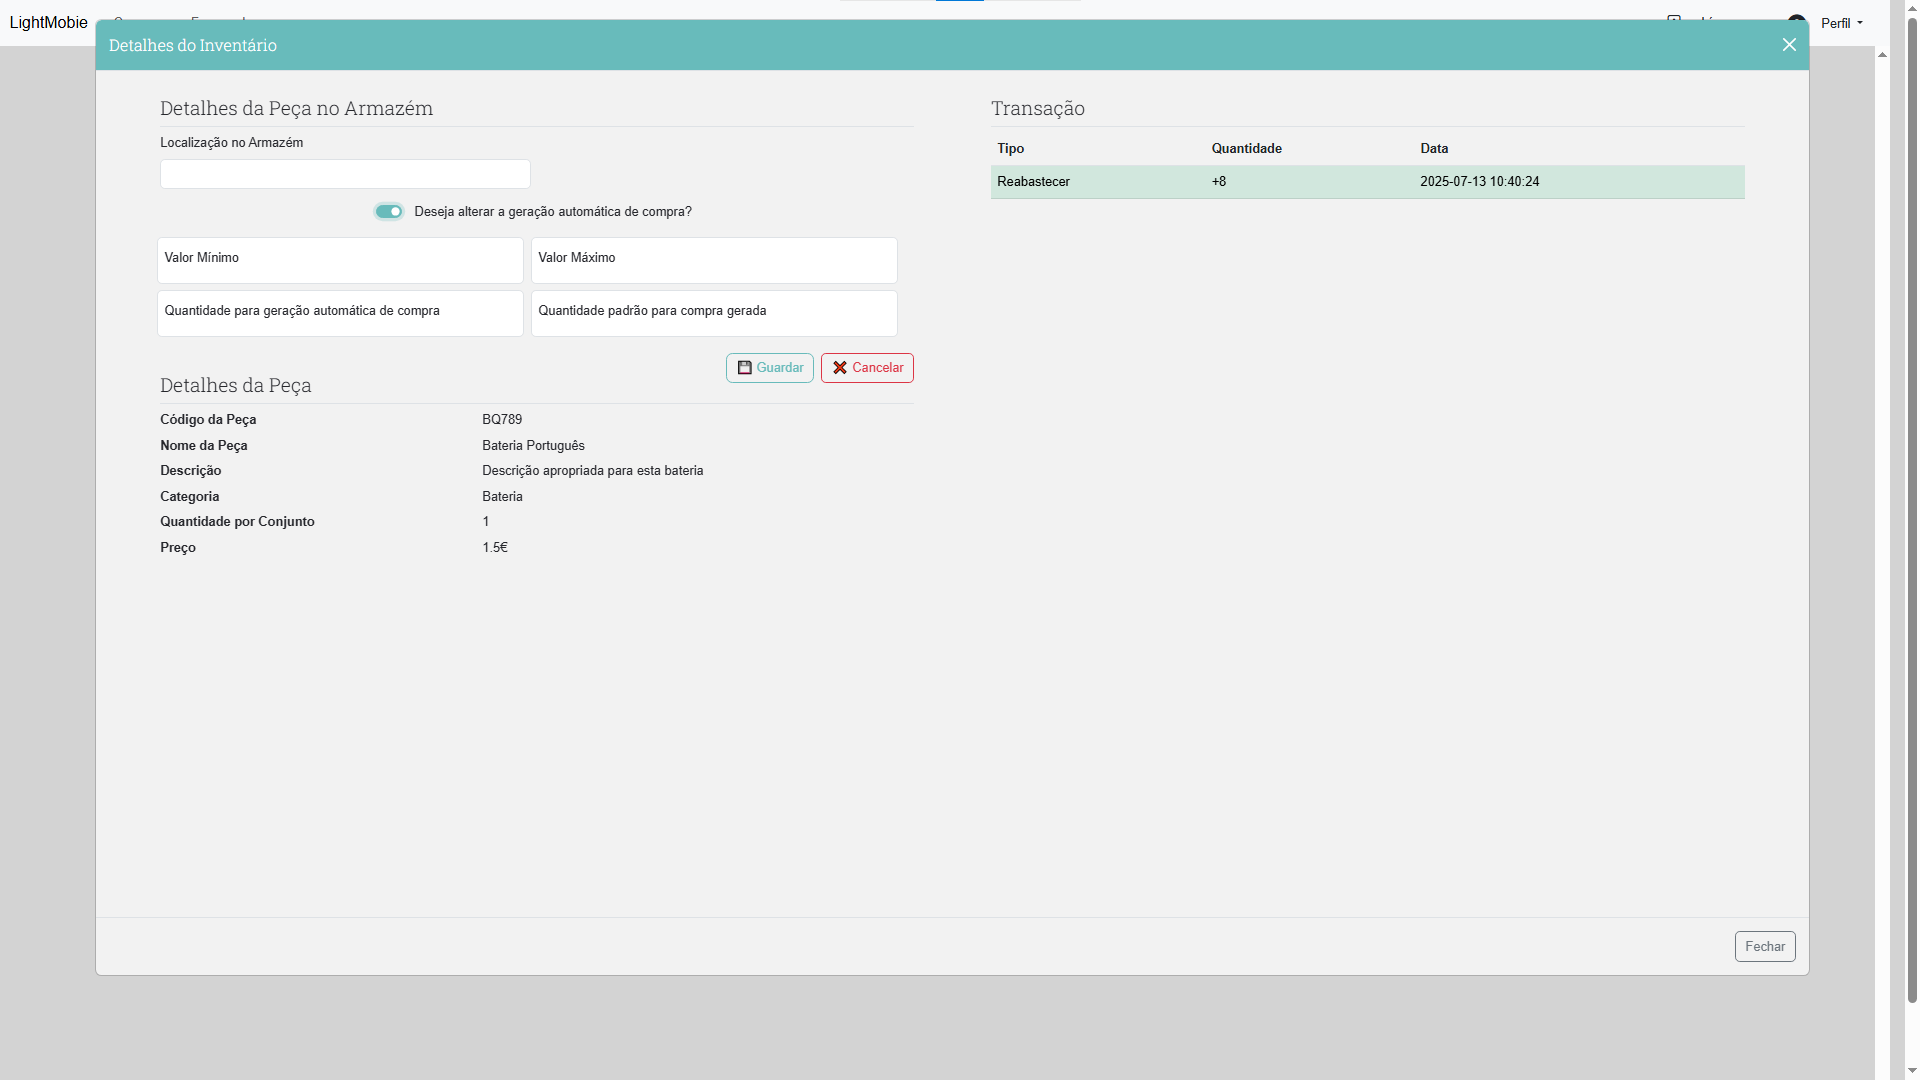
\includegraphics[width=\textwidth]{figs/Implementation/warehouse/inventoryEdit}
  \label{fig:inventoryEdit}
\end{figure}



\begin{figure}[htbp]
  \caption{Assgined purchase details.}
  \centering
  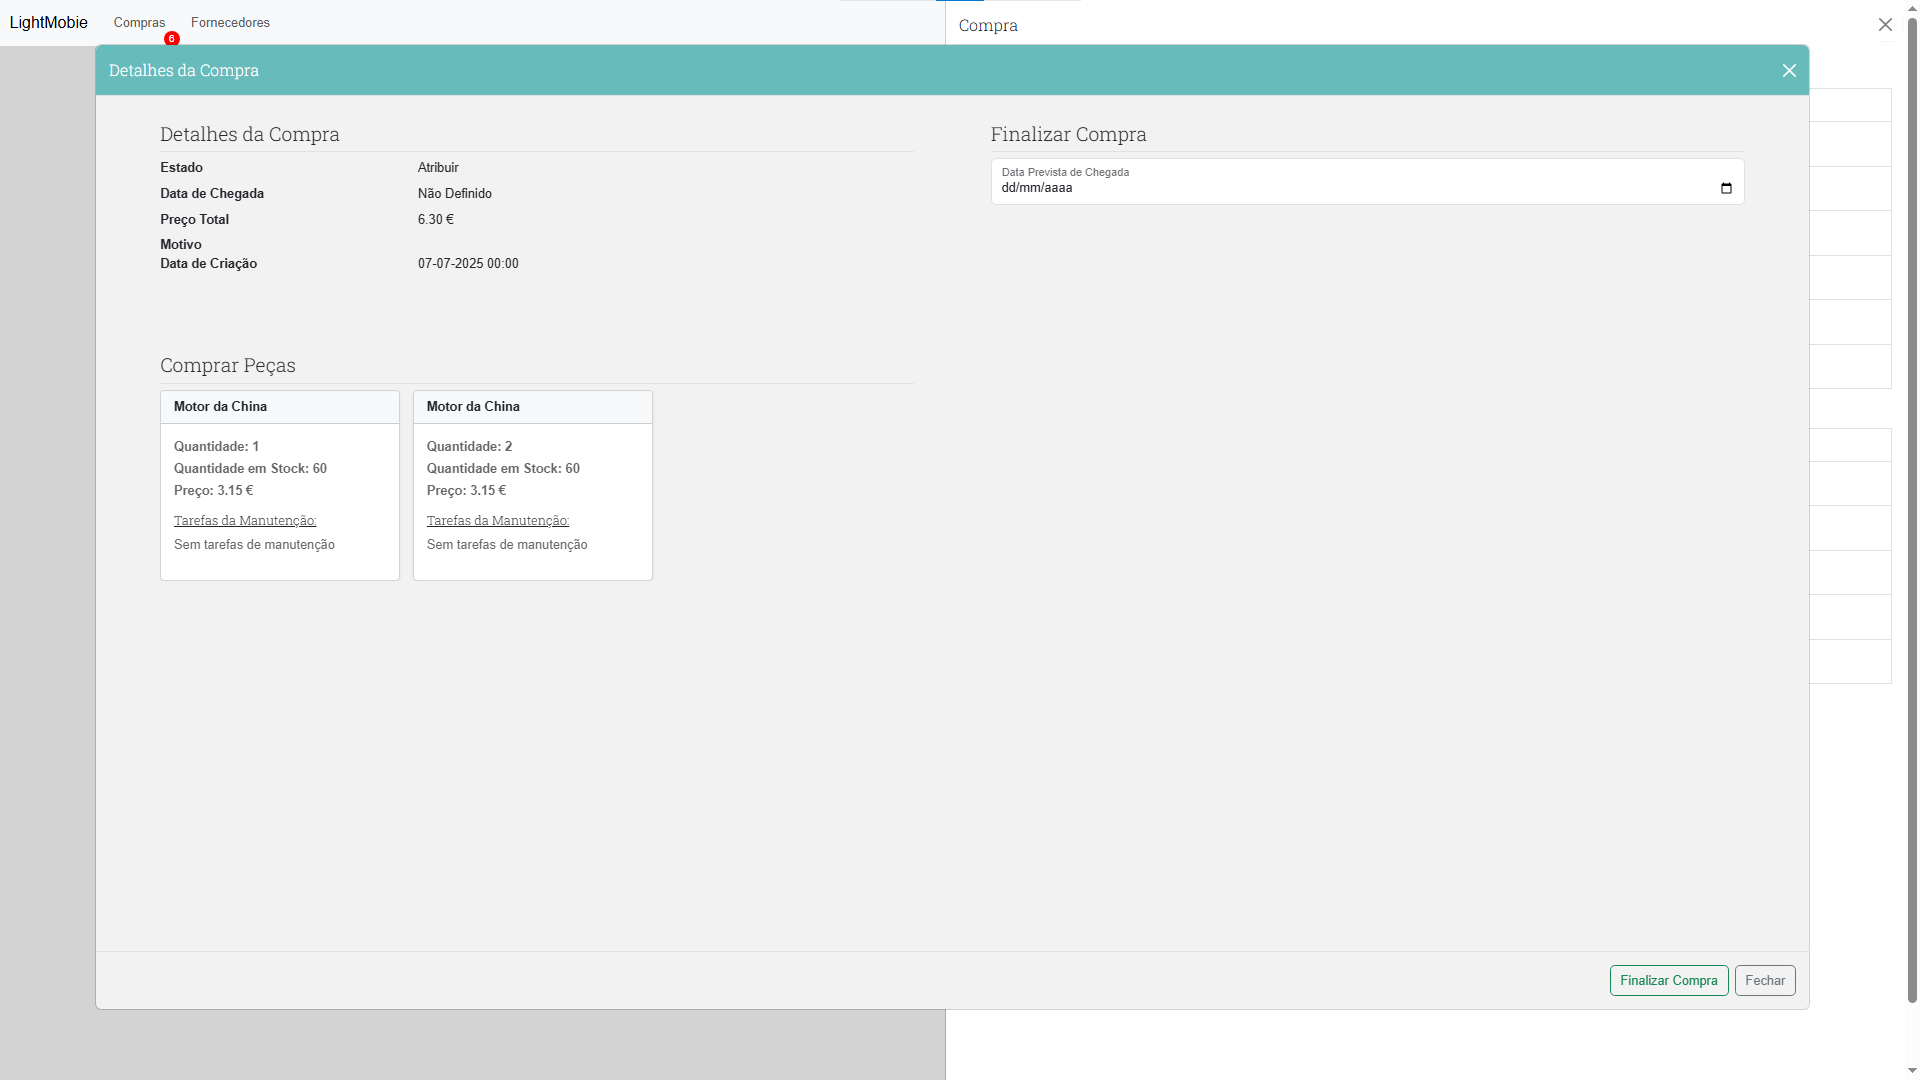
\includegraphics[width=\textwidth]{figs/Implementation/warehouse/PurchaseDetails}
  \label{fig:PurchaseDetails}
\end{figure}


\begin{figure}[htbp]
  \caption{Waiting delivery purchase details.}
  \centering
  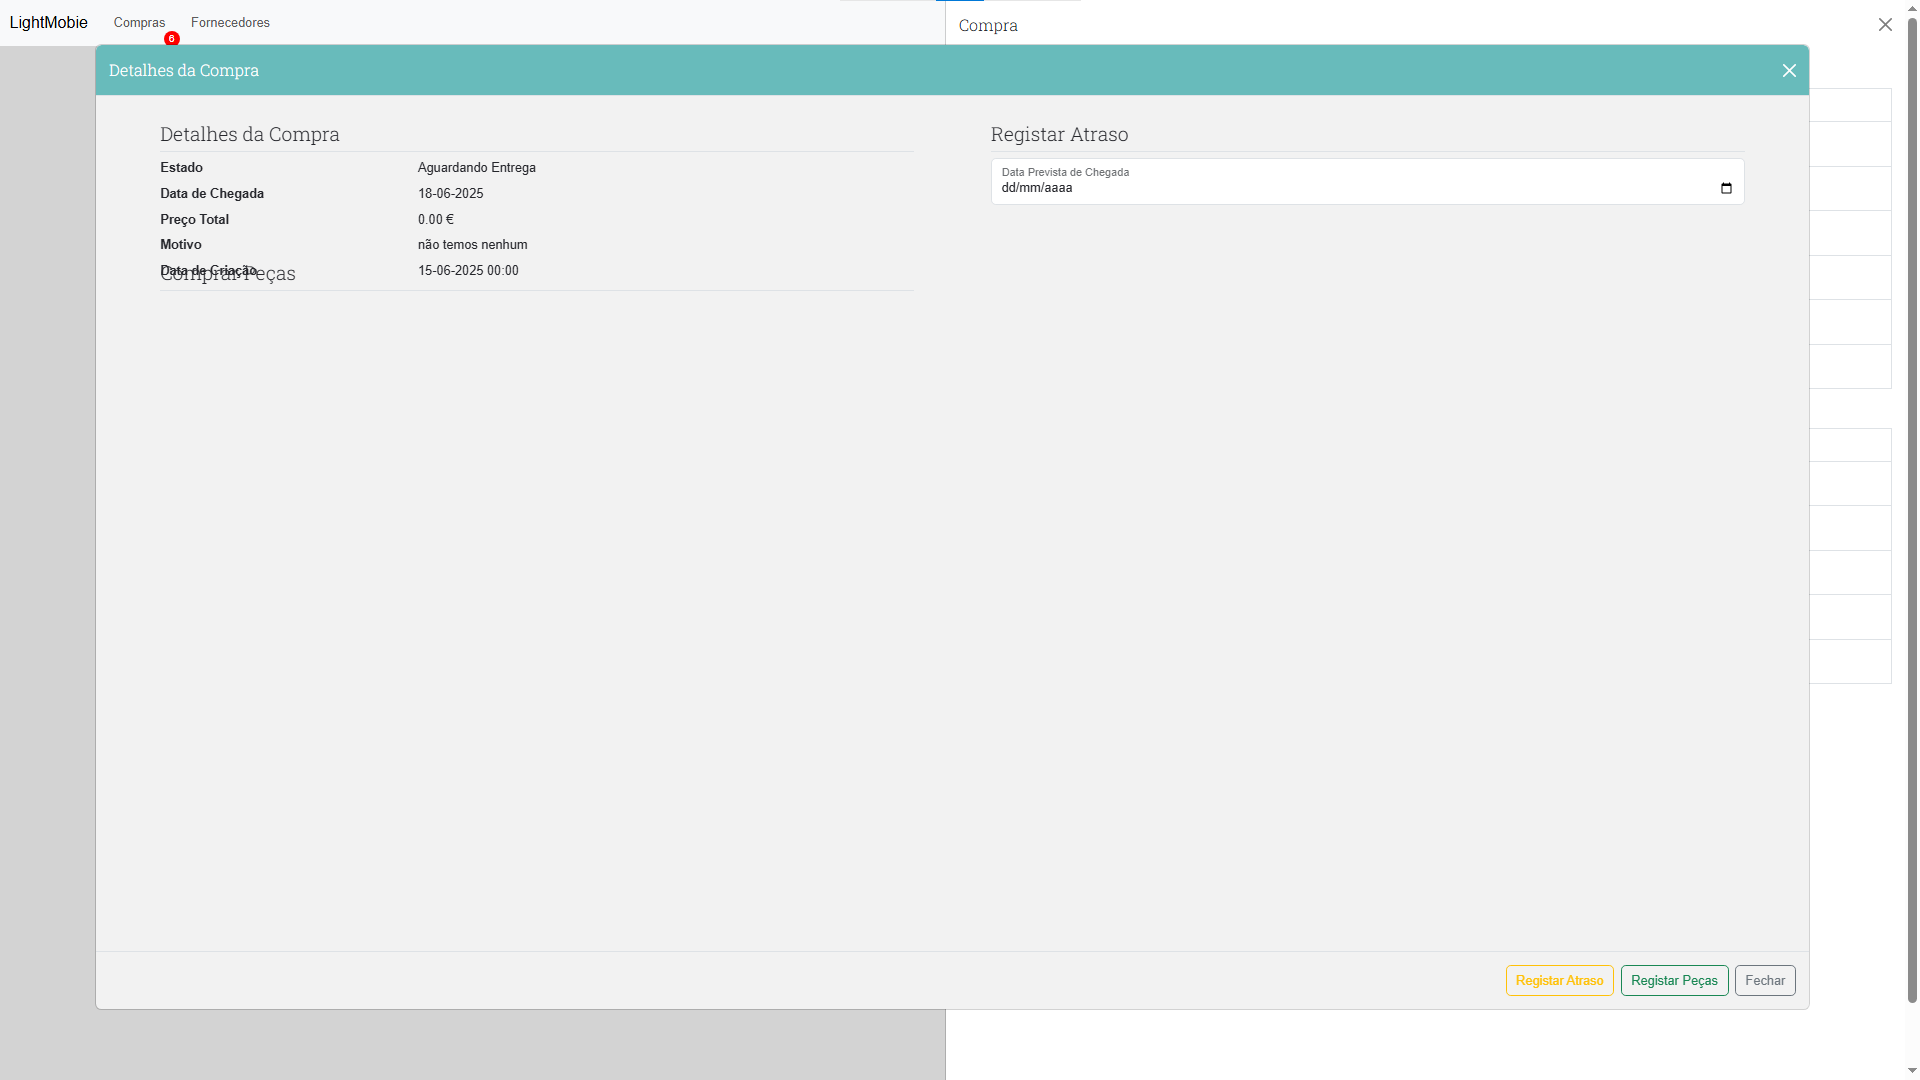
\includegraphics[width=\textwidth]{figs/Implementation/warehouse/PurchaseRegisterParts}
  \label{fig:PurchaseRegisterParts}
\end{figure}


\begin{figure}[htbp]
  \caption{Delivered purchase details.}
  \centering
  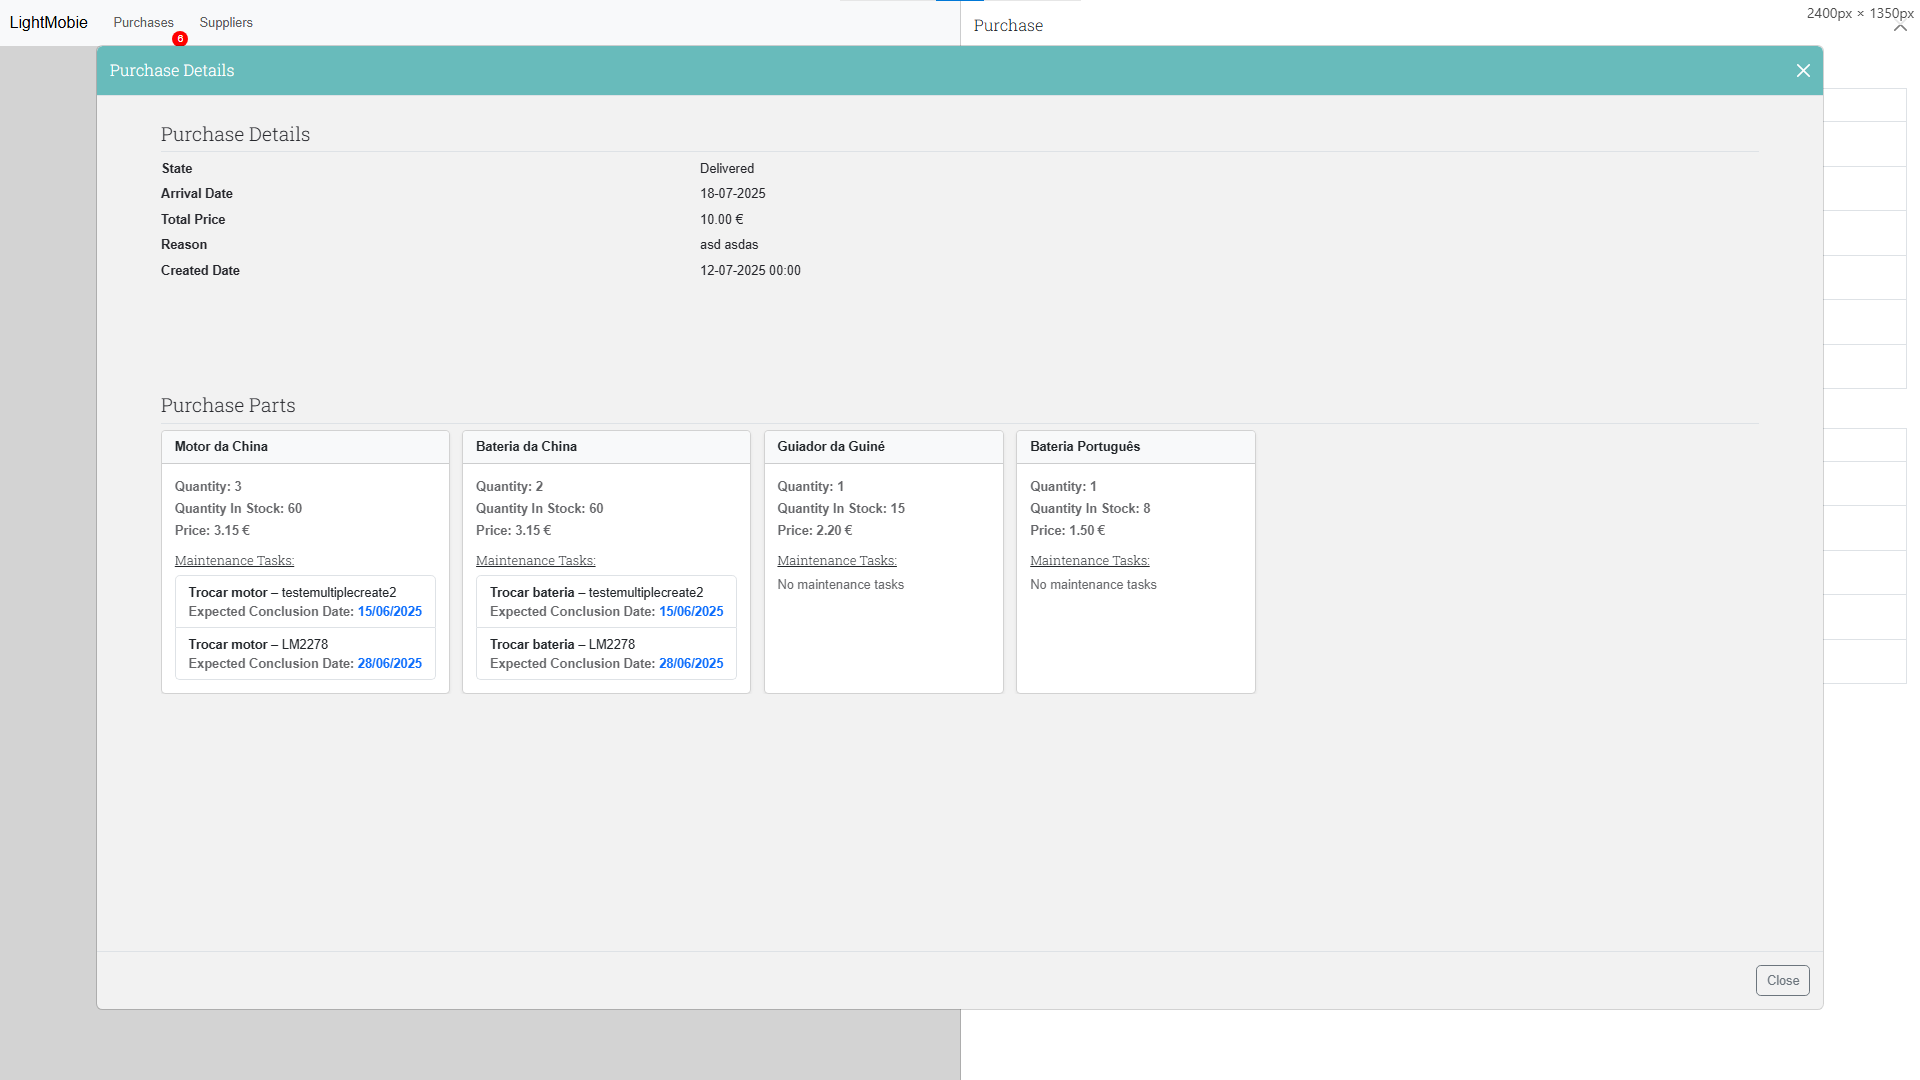
\includegraphics[width=\textwidth]{figs/Implementation/warehouse/PurchaseFinishedDetails}
  \label{fig:PurchaseFinishedDetails}
\end{figure}



\begin{figure}[htbp]
  \caption{Supplier details.}
  \centering
  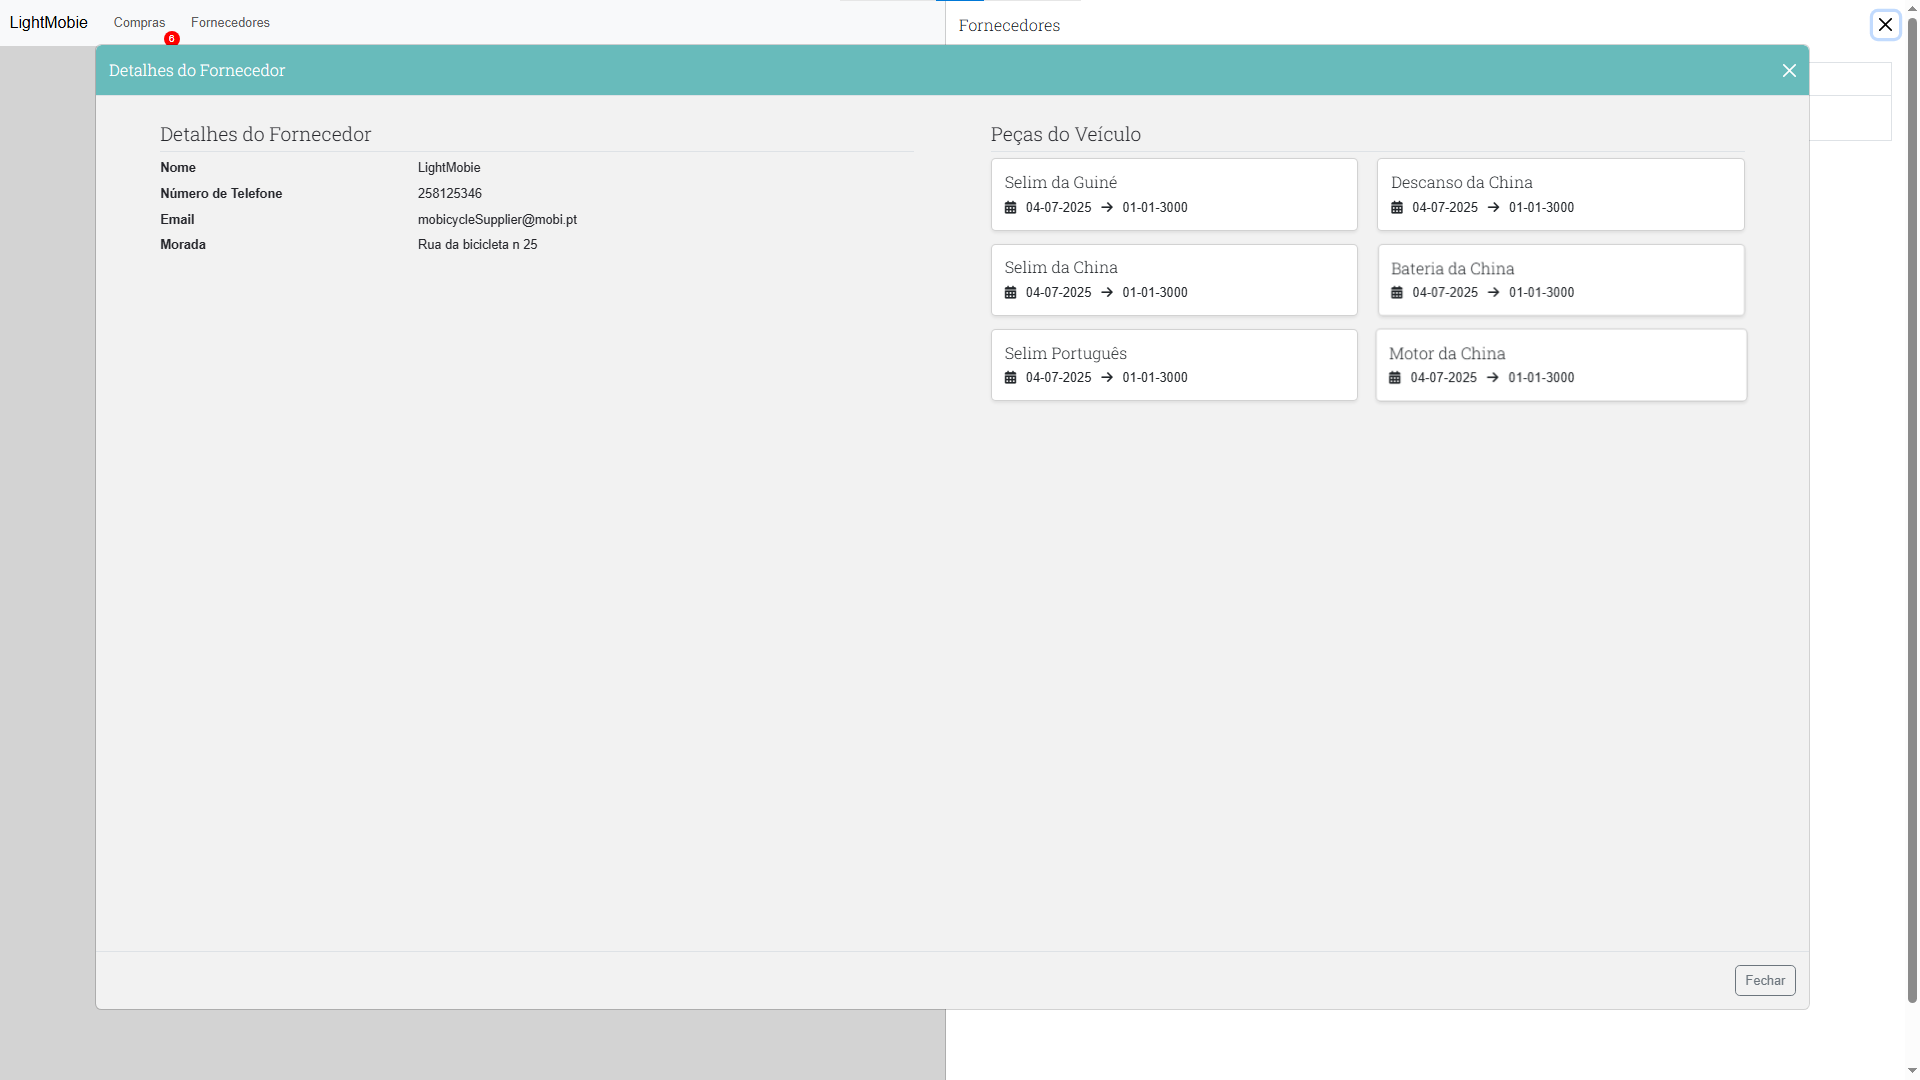
\includegraphics[width=\textwidth]{figs/Implementation/warehouse/supplierDetails}
  \label{fig:supplierDetails}
\end{figure}




\begin{figure}[htbp]
  \caption{Assign task to a mechanic.}
  \centering
  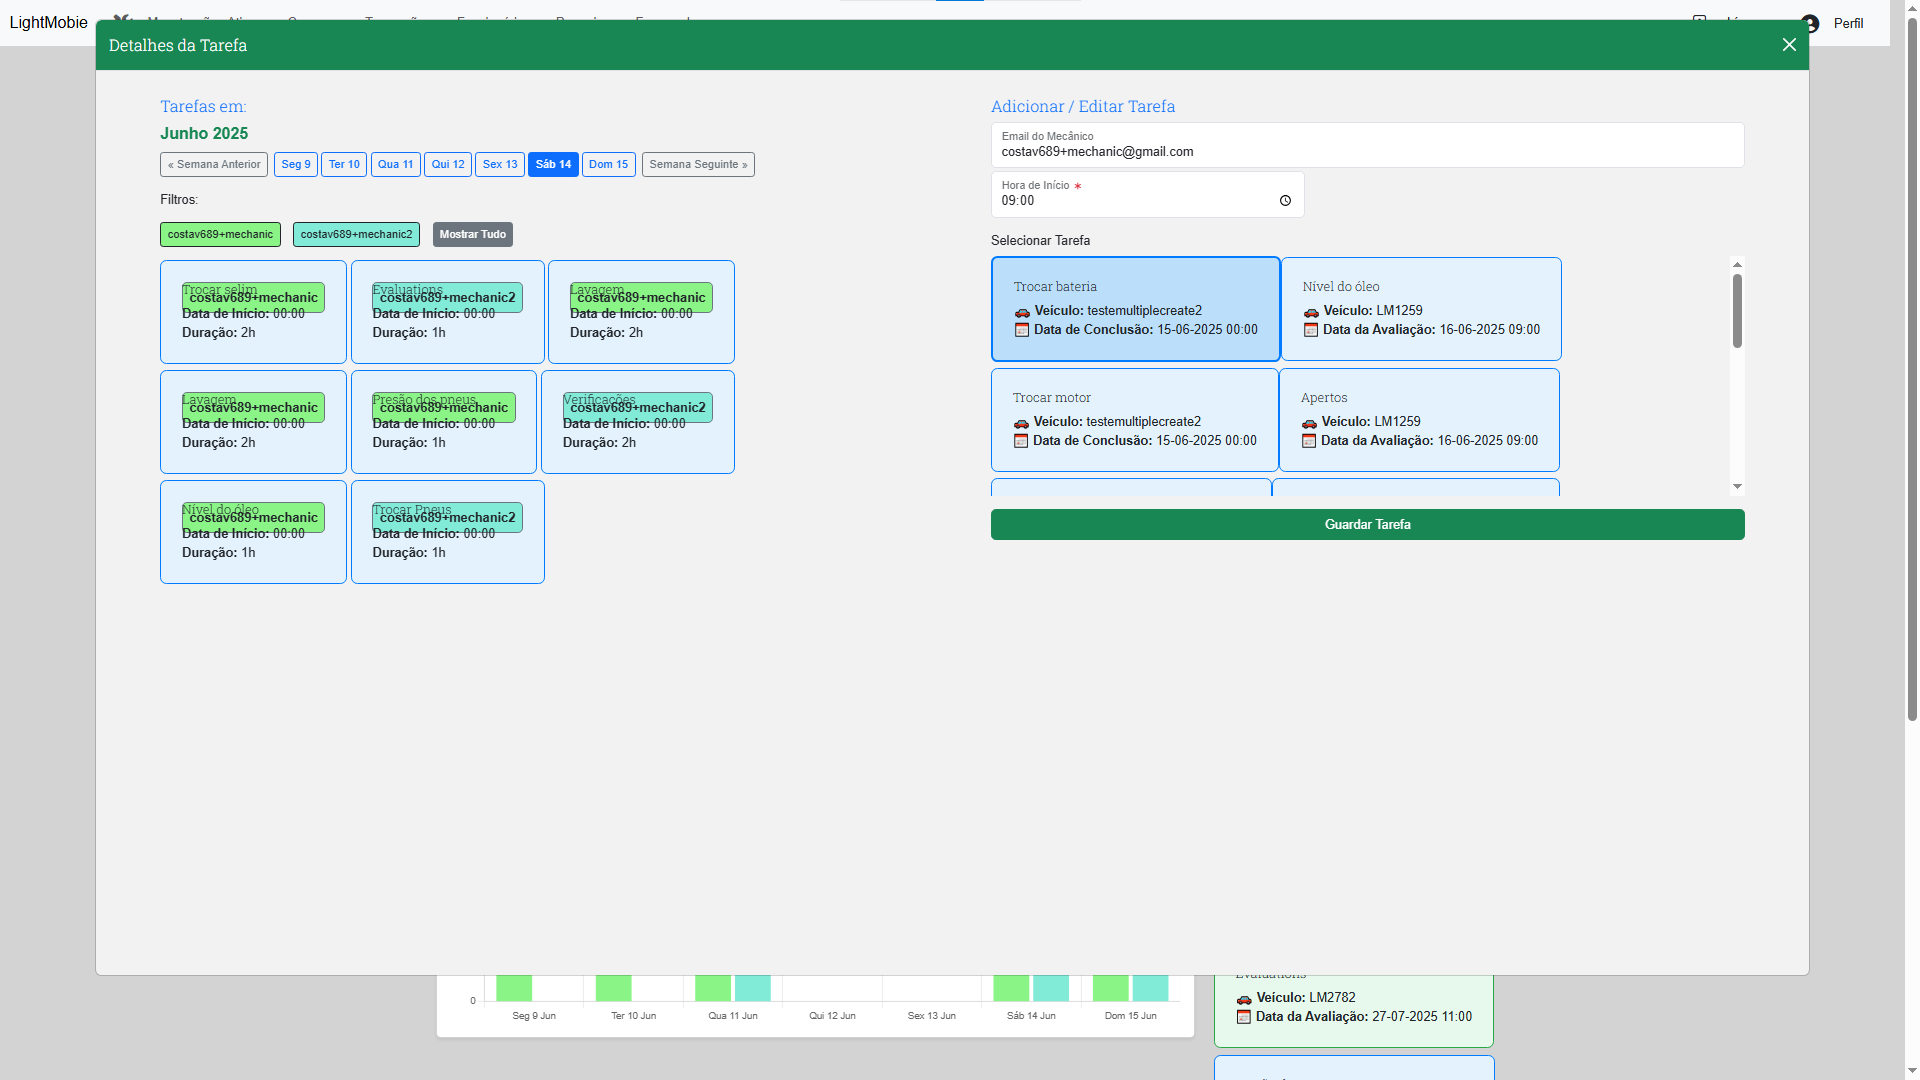
\includegraphics[width=\textwidth]{figs/Implementation/workshopmanager/addTask}
  \label{fig:workshopmanagerAssignTask}
\end{figure}


\begin{figure}[htbp]
  \caption{Active maintenance list.}
  \centering
  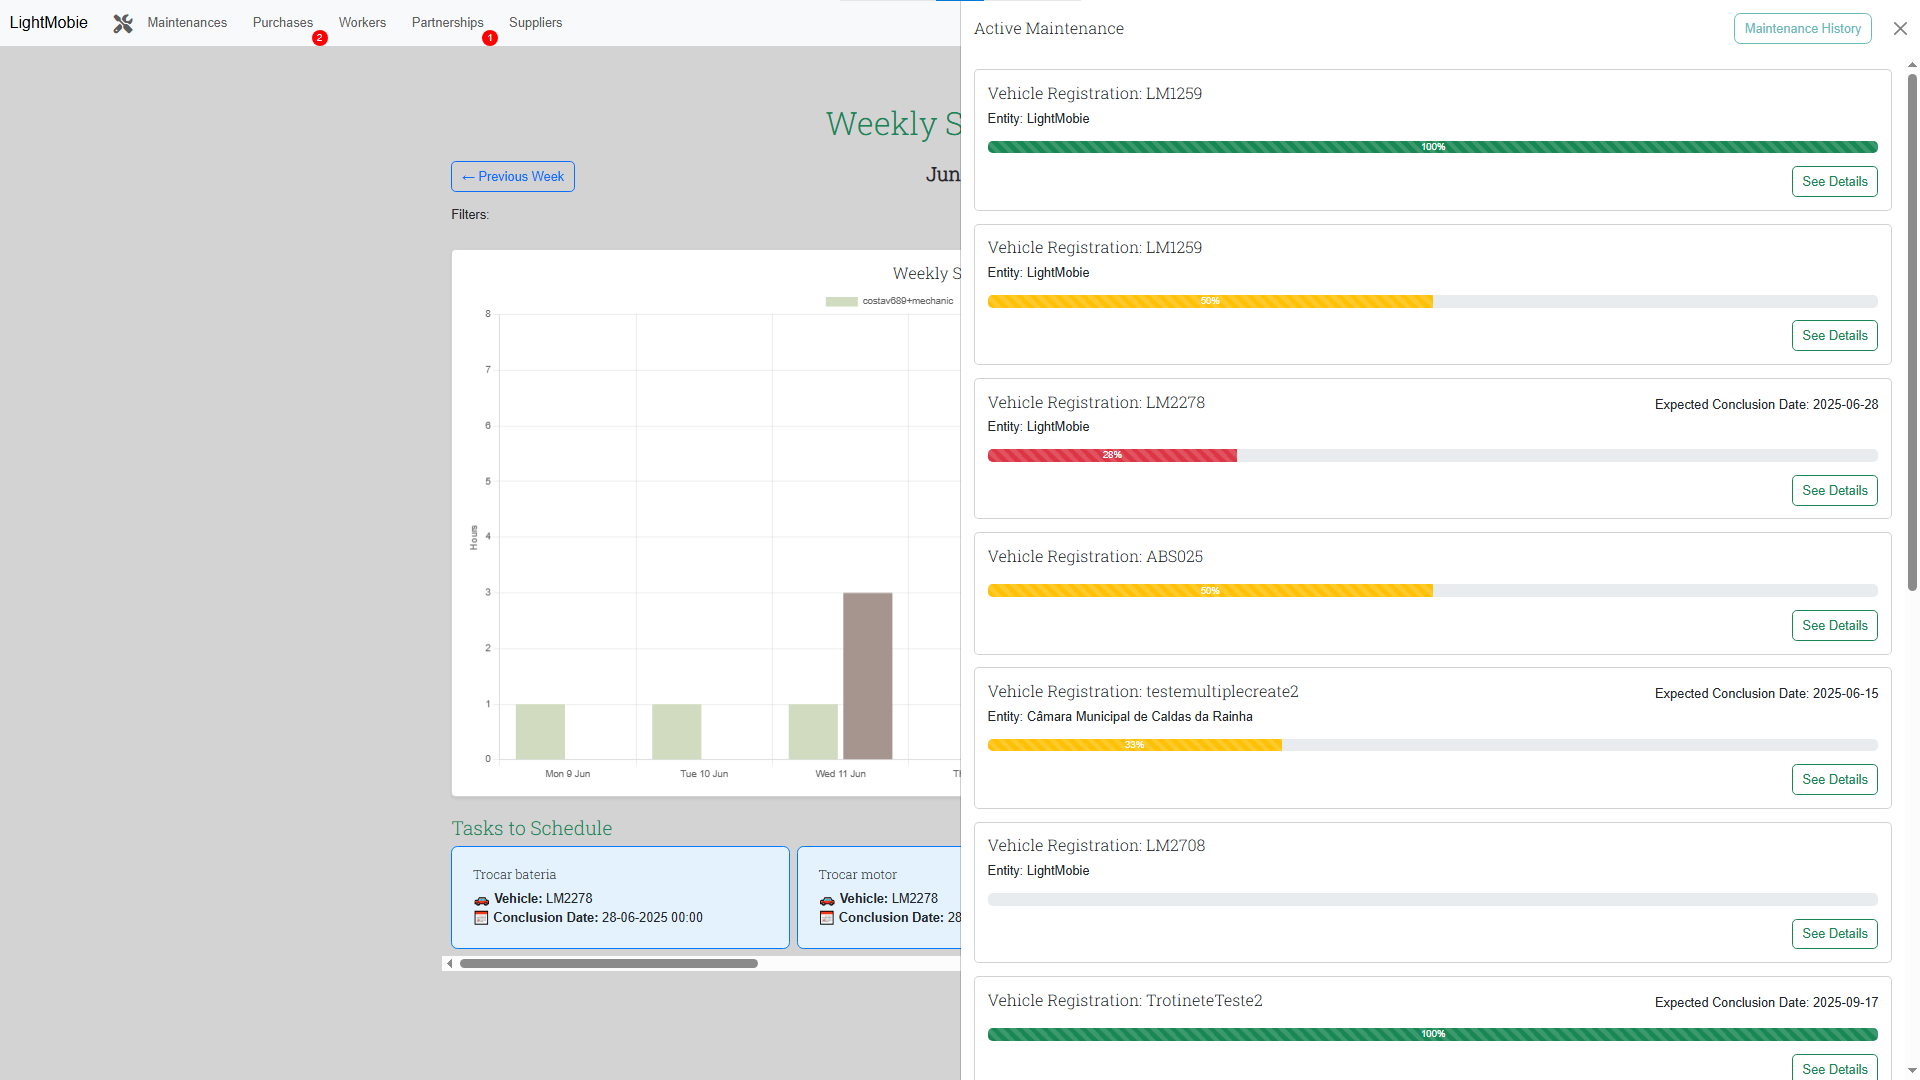
\includegraphics[width=\textwidth]{figs/Implementation/workshopmanager/maintenanceList}
  \label{fig:workshopmanagerMaintenanceList}
\end{figure}


\begin{figure}[htbp]
  \caption{Maintenance details information tab.}
  \centering
  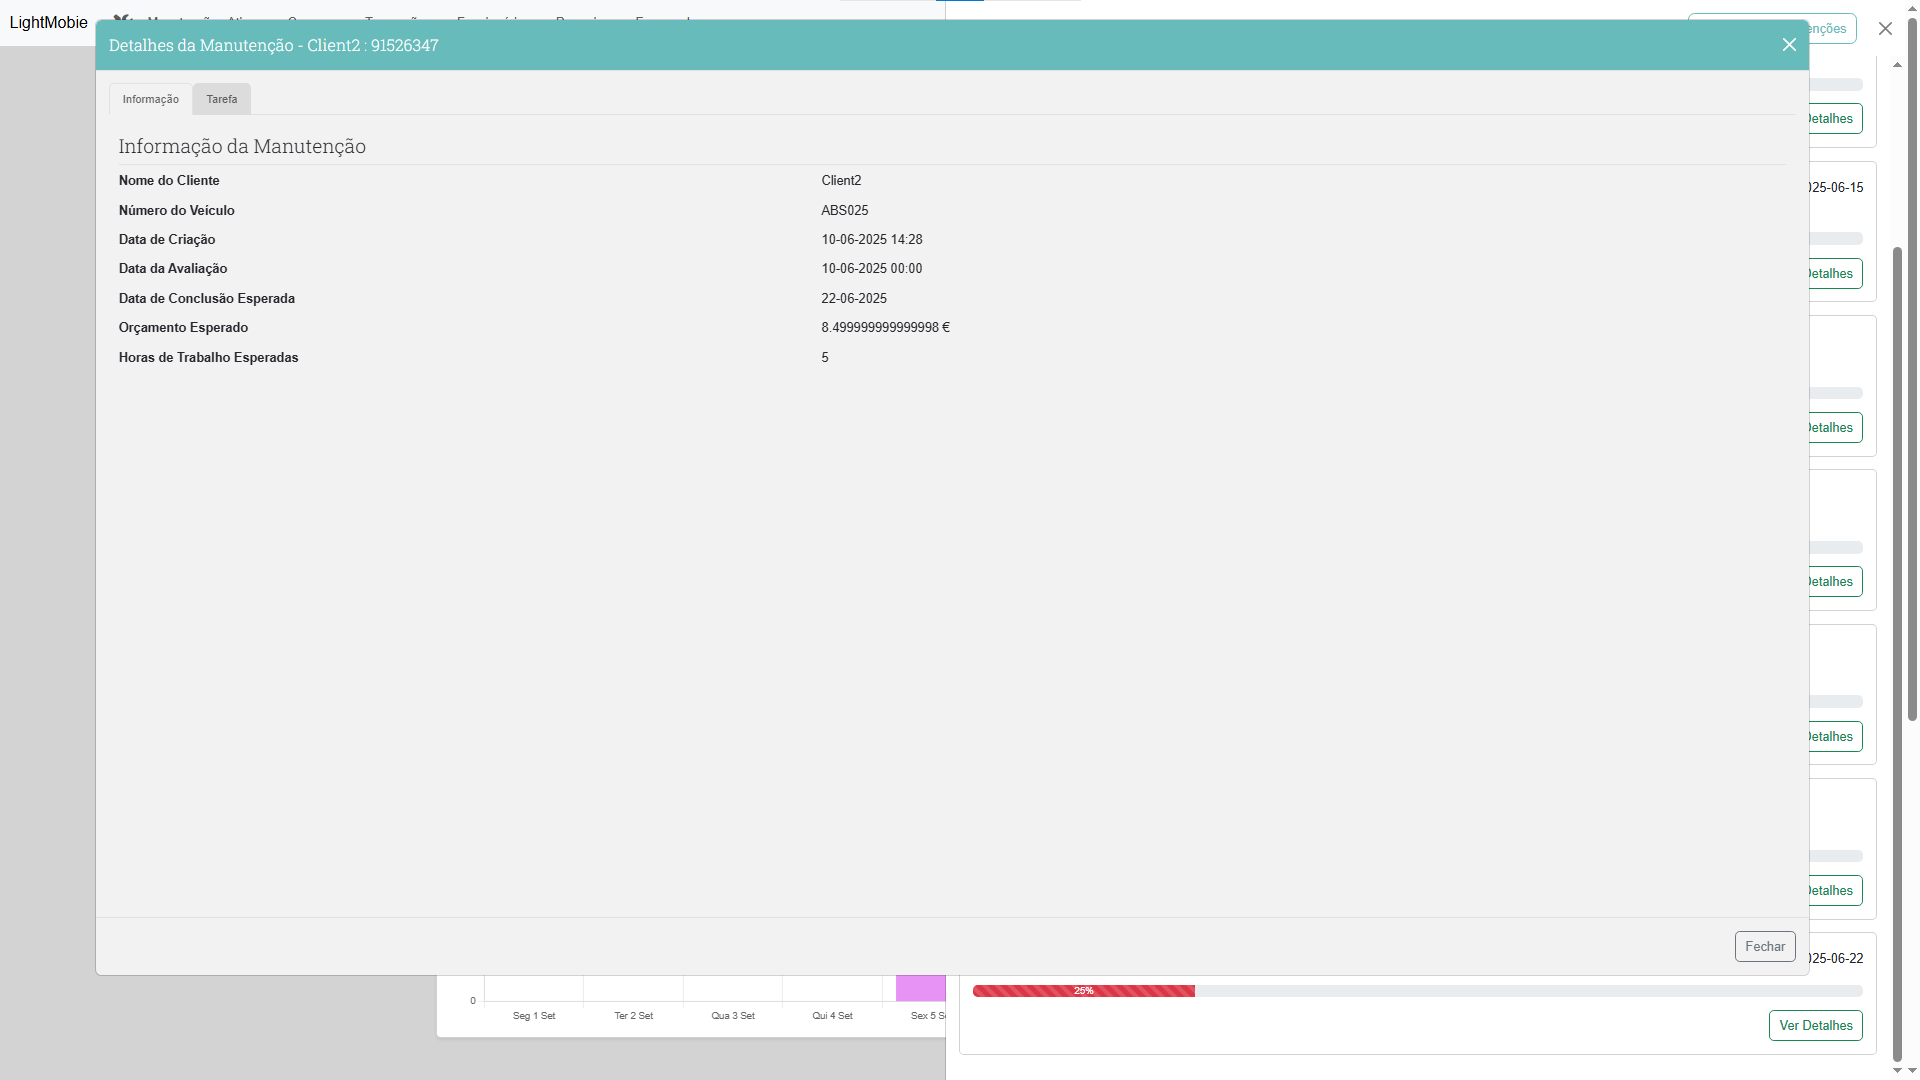
\includegraphics[width=\textwidth]{figs/Implementation/workshopmanager/maintenanceDetails}
  \label{fig:workshopmanagerMaintenanceDetails}
\end{figure}

\begin{figure}[htbp]
  \caption{Maintenance details tasks tab.}
  \centering
  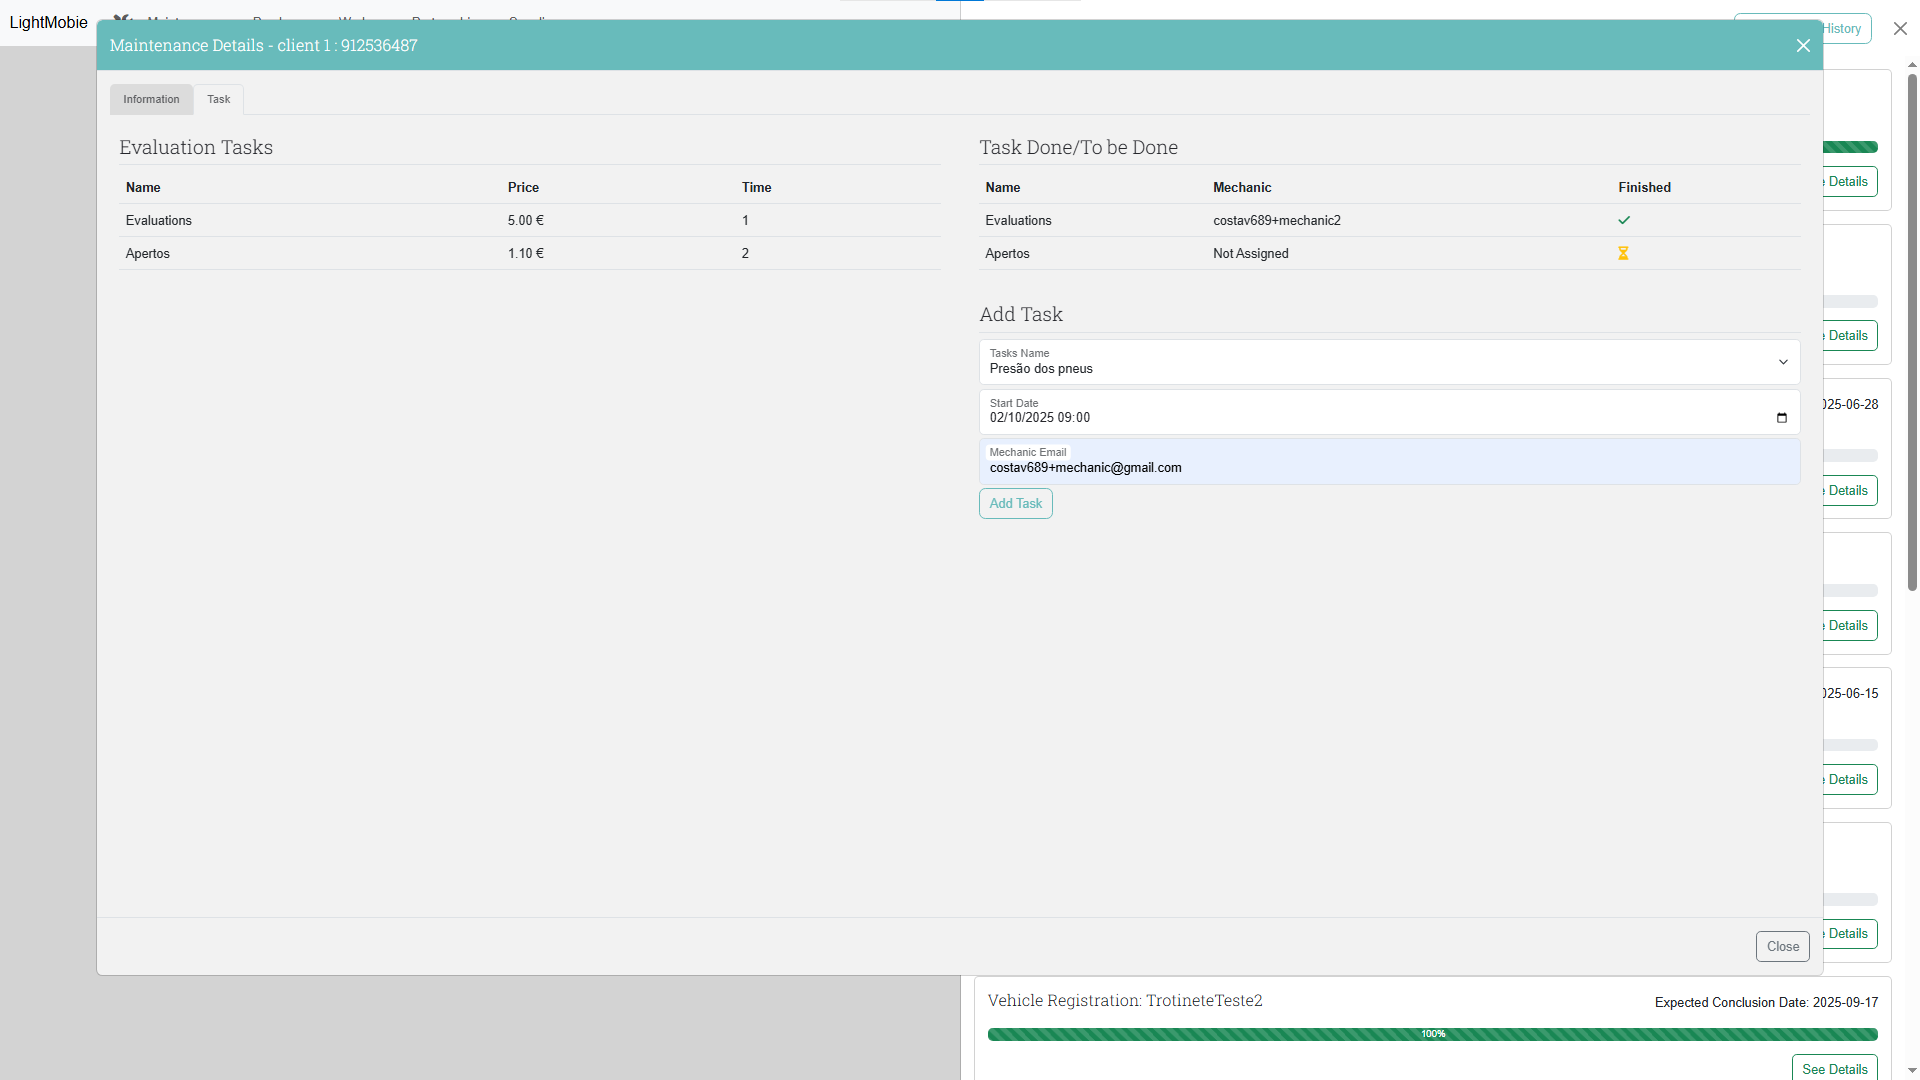
\includegraphics[width=\textwidth]{figs/Implementation/workshopmanager/maintenanceDetailsTask}
  \label{fig:workshopmanagerMaintenanceDetailsTask}
\end{figure}


\begin{figure}[htbp]
  \caption{Report example.}
  \centering
  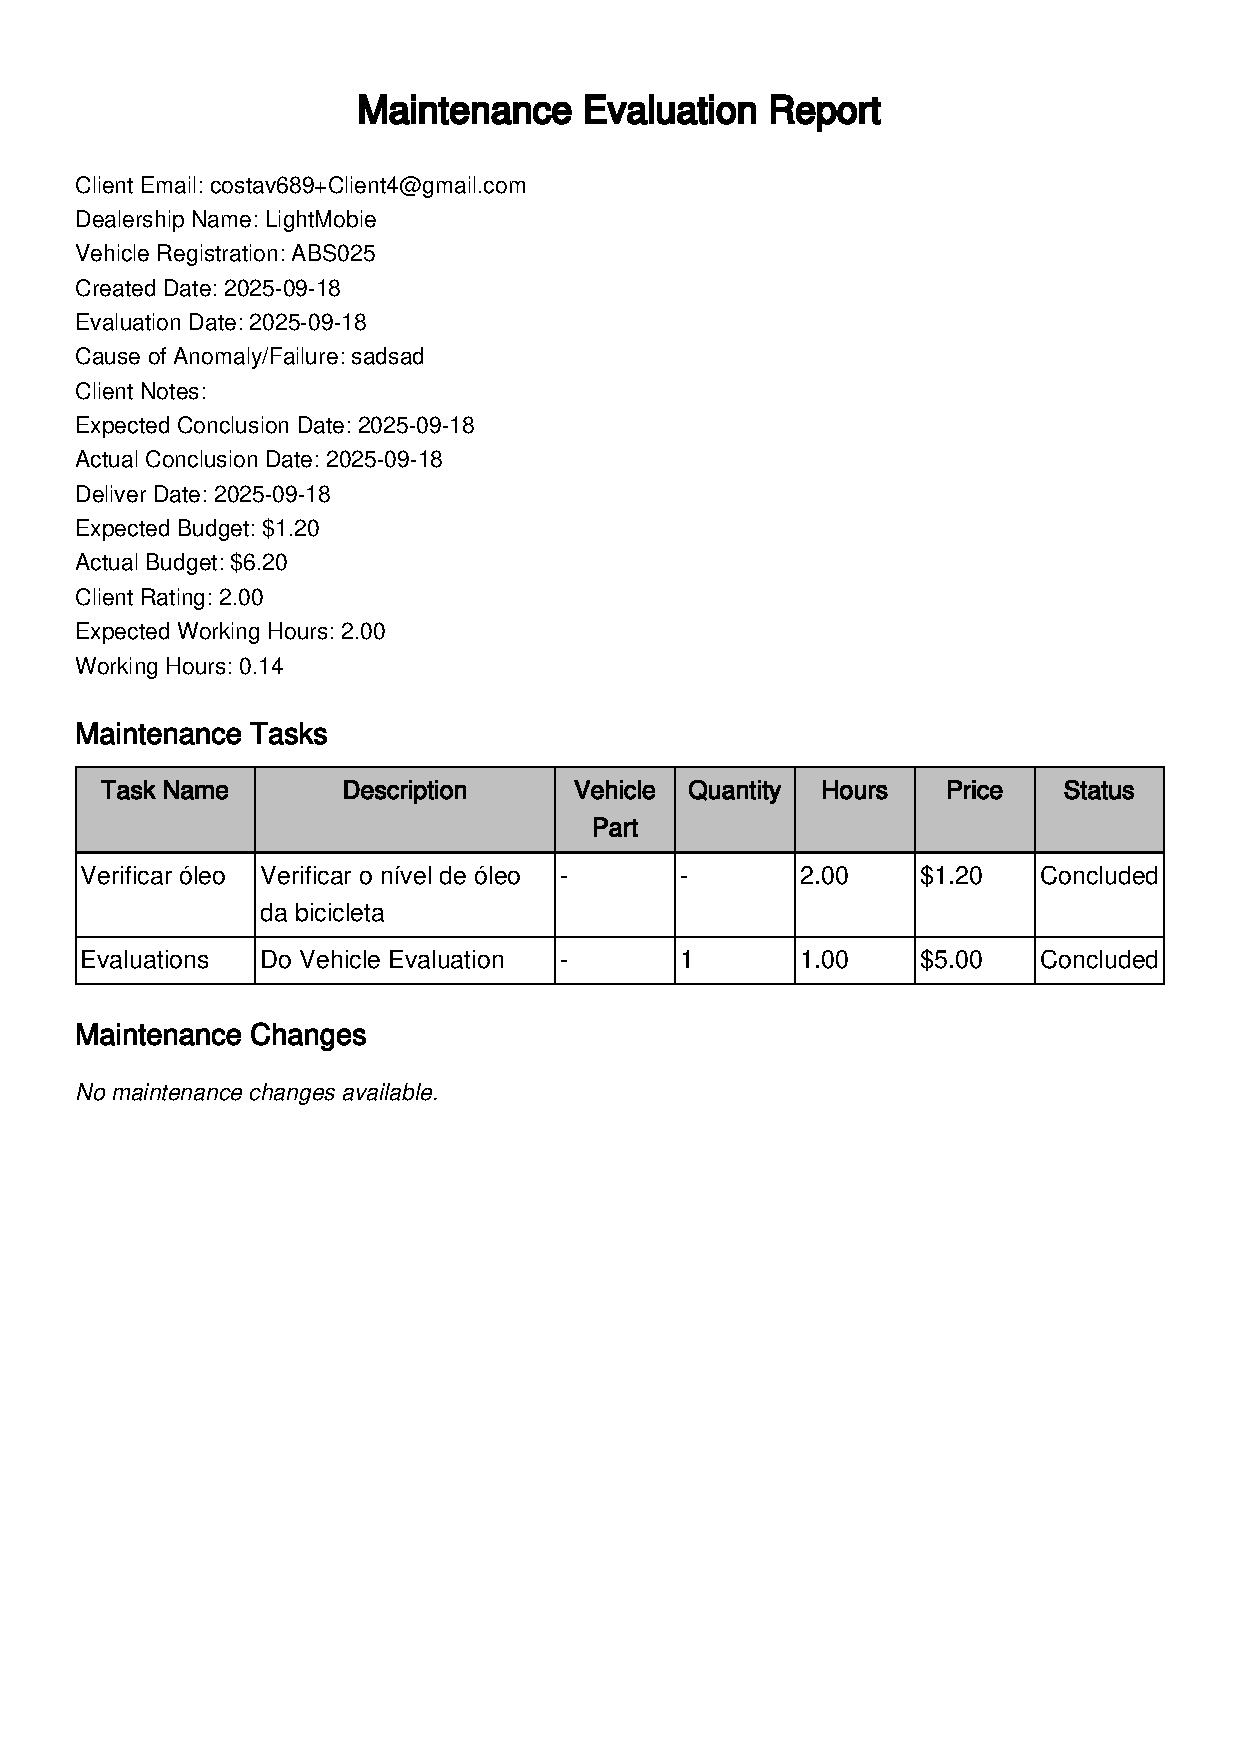
\includegraphics[width=\textwidth]{figs/Implementation/workshopmanager/report}
  \label{fig:report}
\end{figure}


 


\begin{figure}[htbp]
  \caption{Purchase request details.}
  \centering
  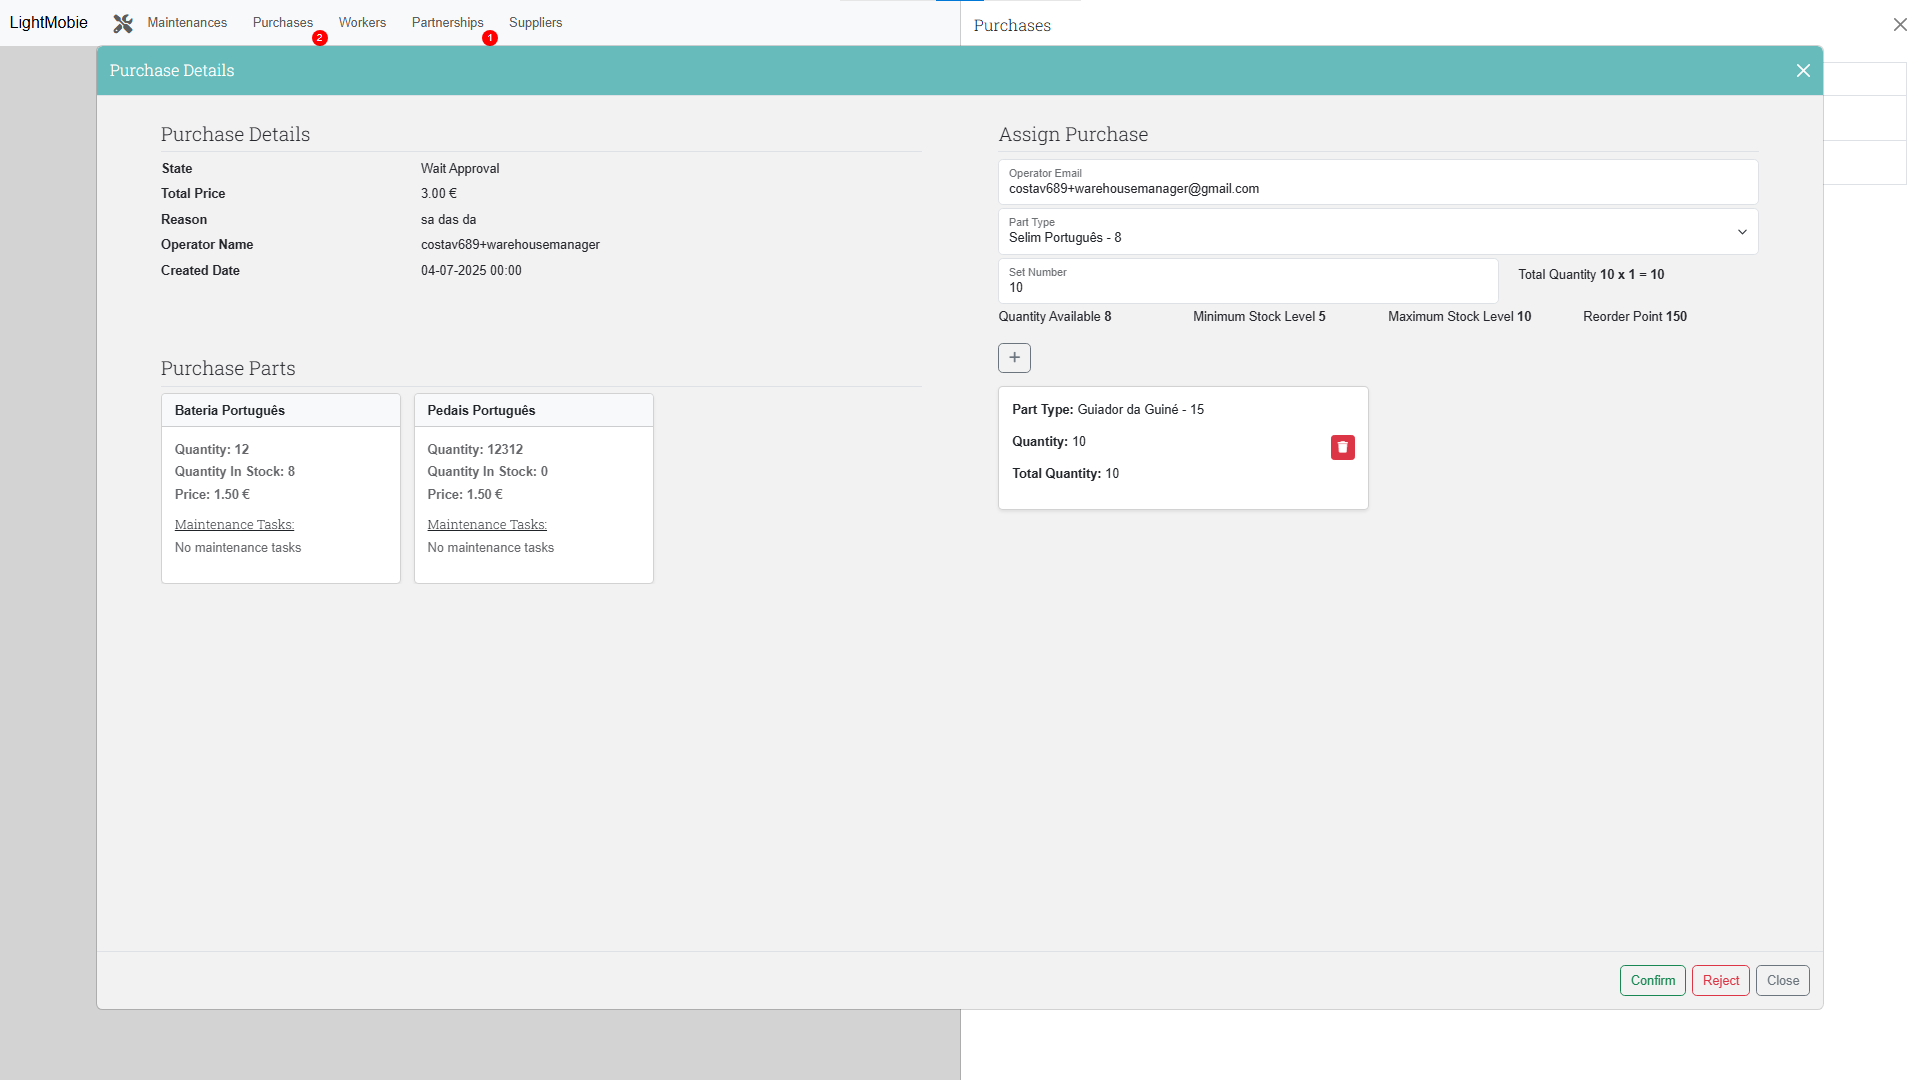
\includegraphics[width=\textwidth]{figs/Implementation/workshopmanager/purchaseDetails}
  \label{fig:workshopmanagerPurchaseDetails}
\end{figure}


\begin{figure}[htbp]
  \caption{Supplier list.}
  \centering
  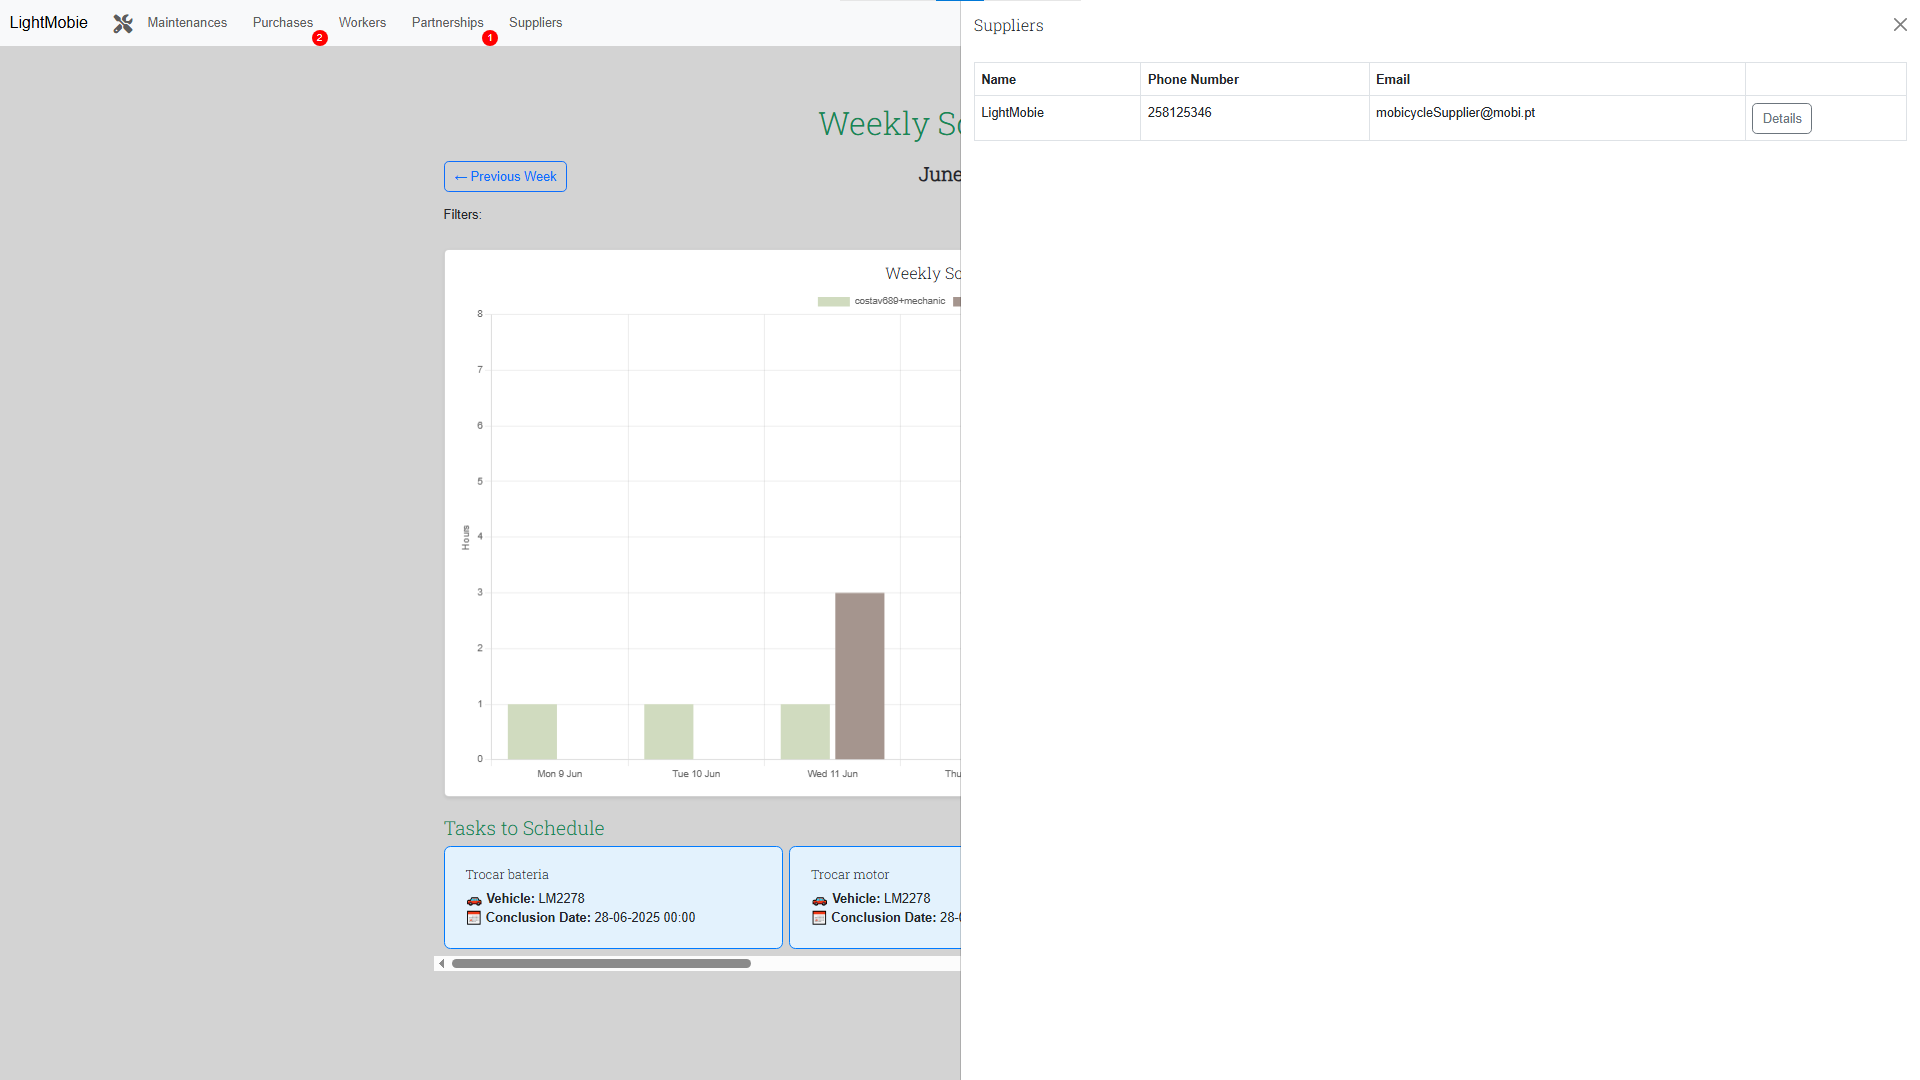
\includegraphics[width=\textwidth]{figs/Implementation/workshopmanager/supplierList}
  \label{fig:workshopmanagerSupplierList}
\end{figure}

\begin{figure}[htbp]
  \caption{Supplier Details.}
  \centering
  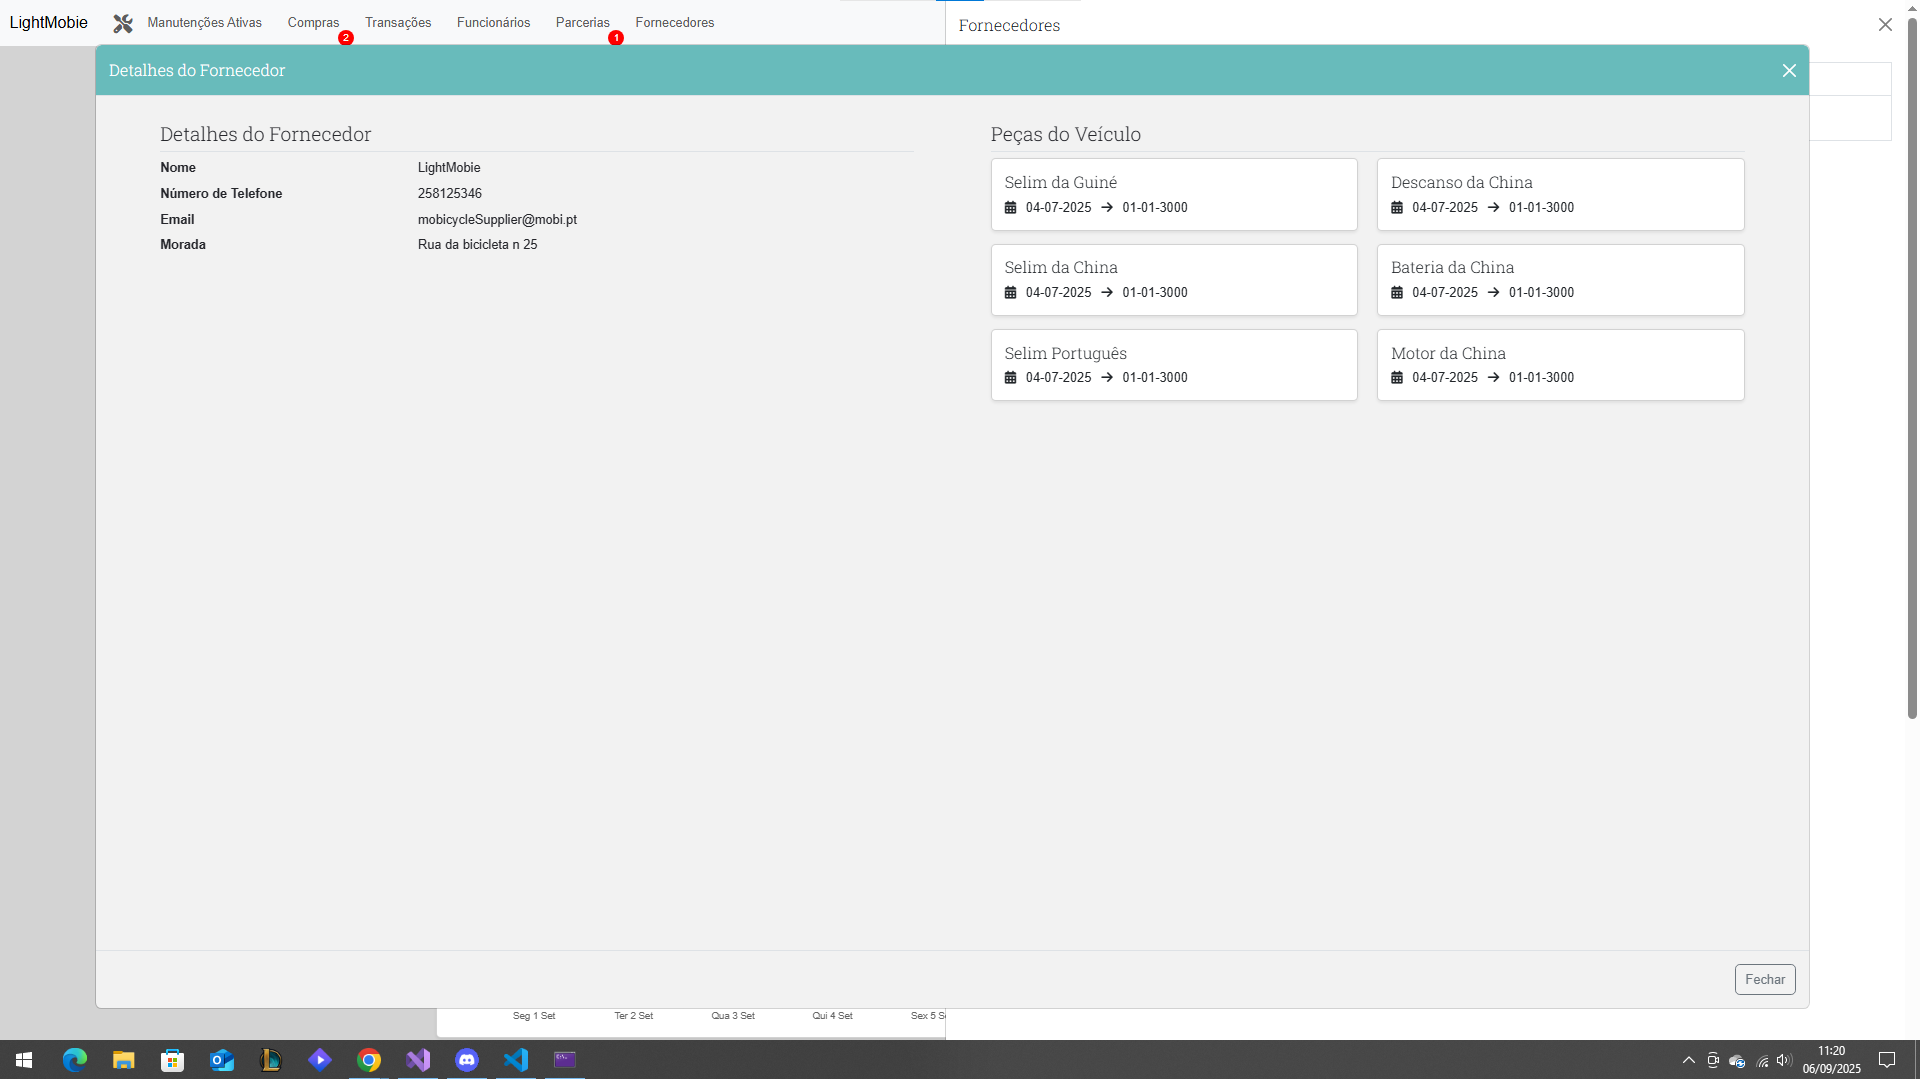
\includegraphics[width=\textwidth]{figs/Implementation/workshopmanager/supplierDetails}
  \label{fig:workshopmanagerupplierDetails}
\end{figure}


\begin{figure}[htbp]
  \caption{Worker details.}
  \centering
  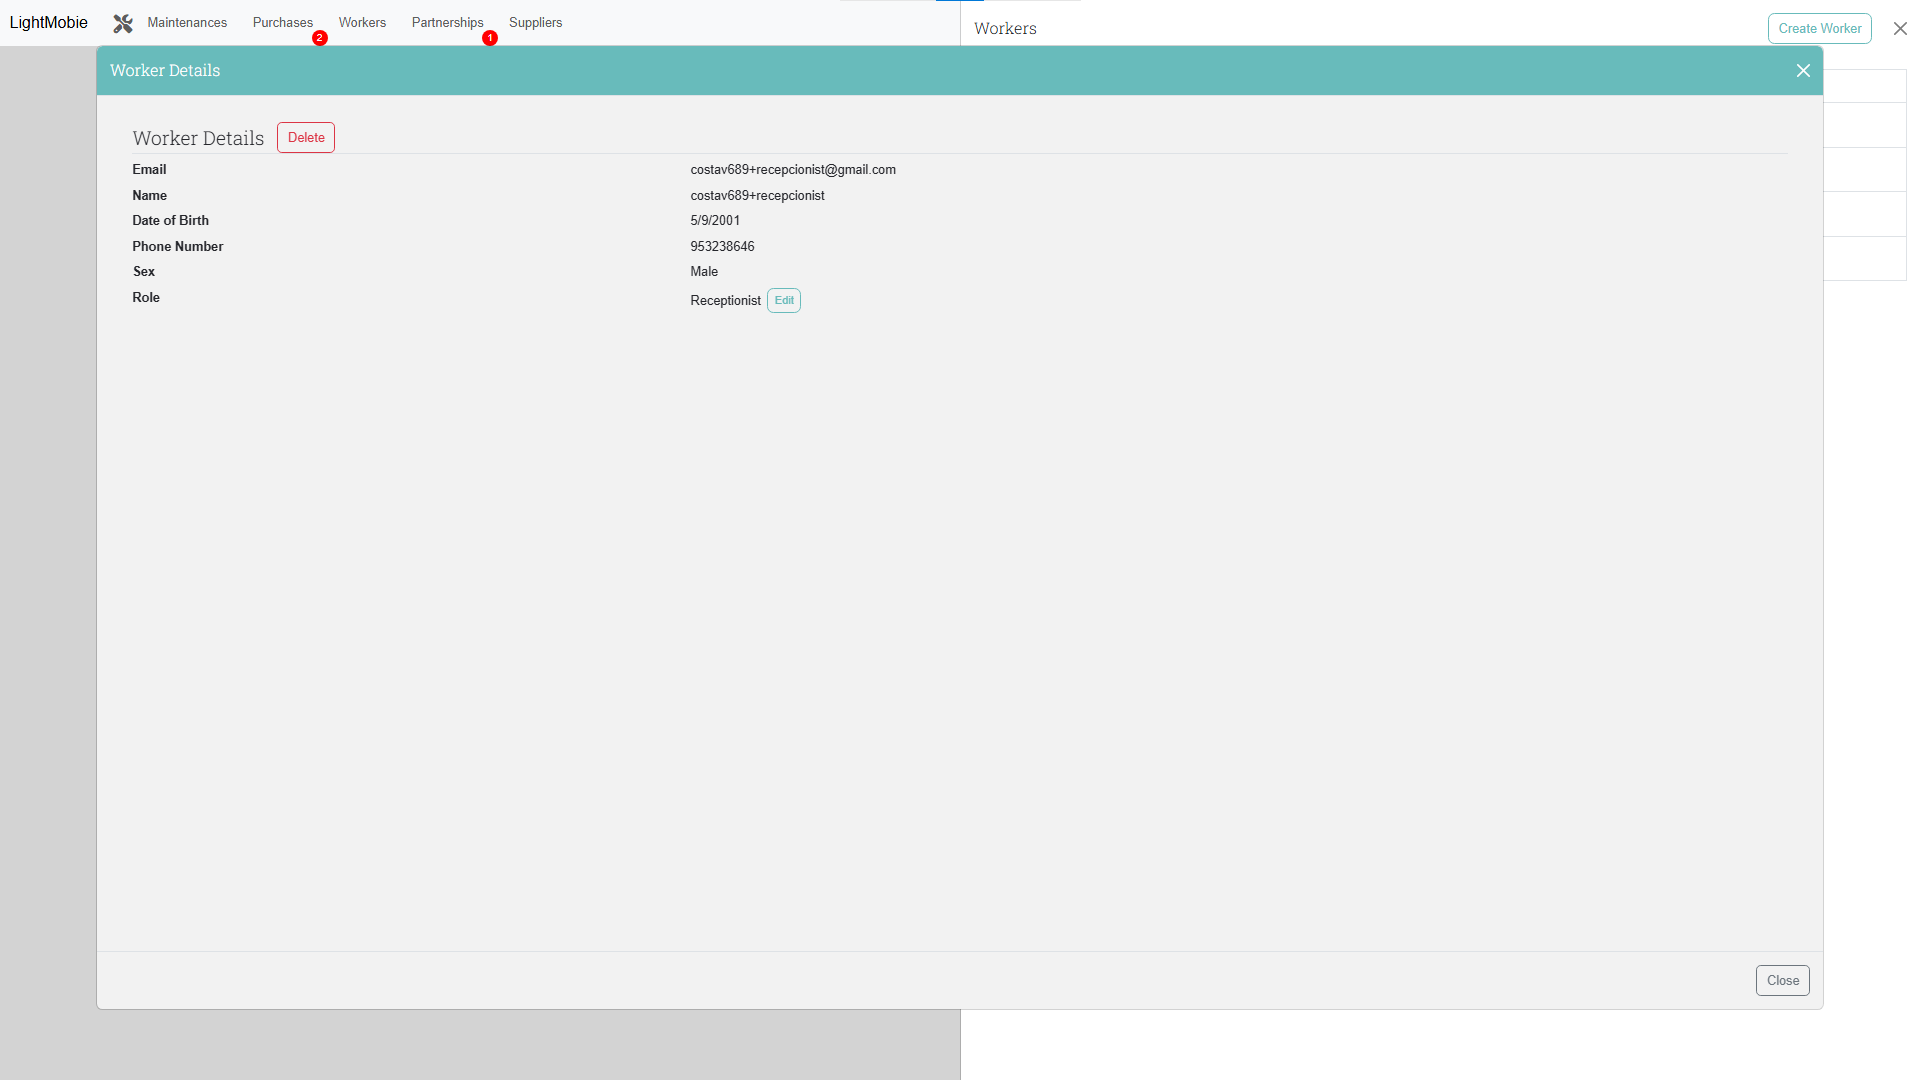
\includegraphics[width=\textwidth]{figs/Implementation/workshopmanager/workerDetails}
  \label{fig:workerDetails}
\end{figure}



\begin{figure}[htbp]
  \caption{Create worker.}
  \centering
  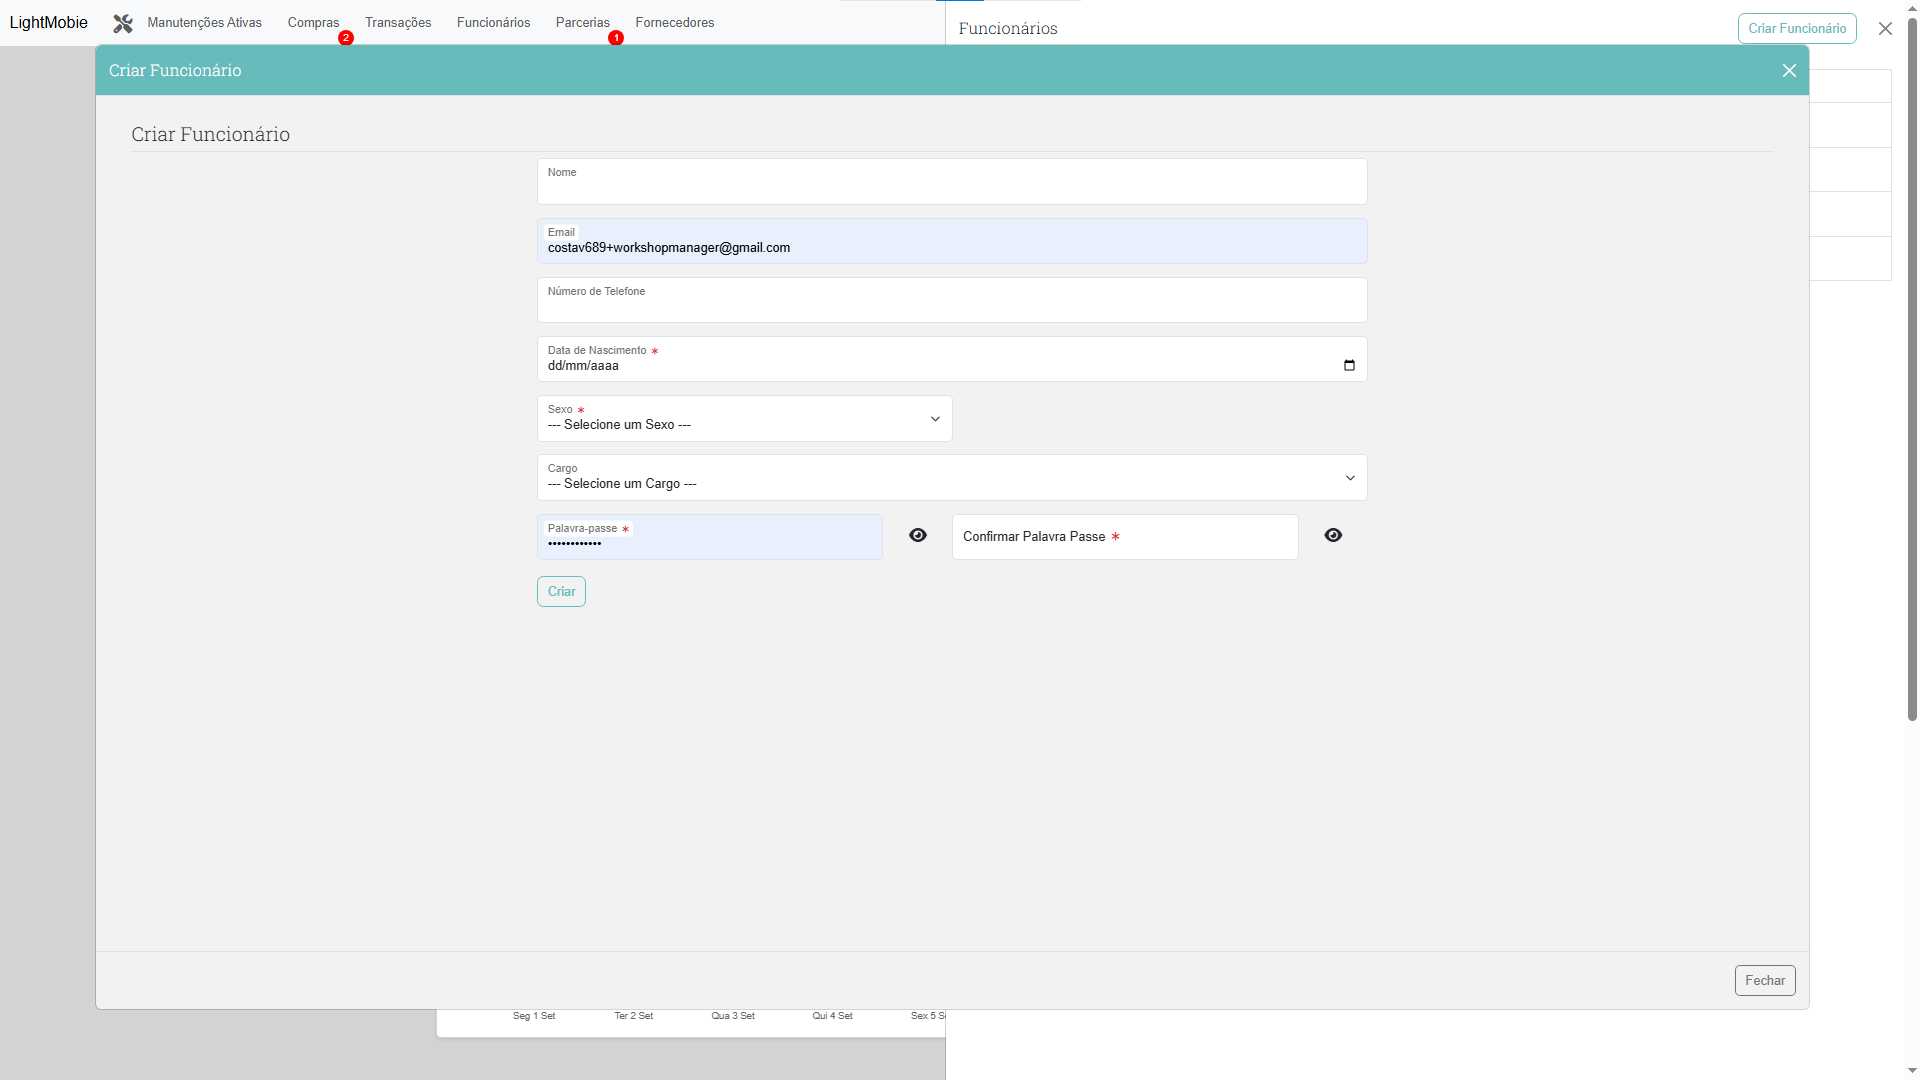
\includegraphics[width=\textwidth]{figs/Implementation/workshopmanager/workerCreate}
  \label{fig:workerCreate}
\end{figure}


\begin{figure}[htbp]
  \caption{Client email notification of the end of the maintenance.}
  \centering
  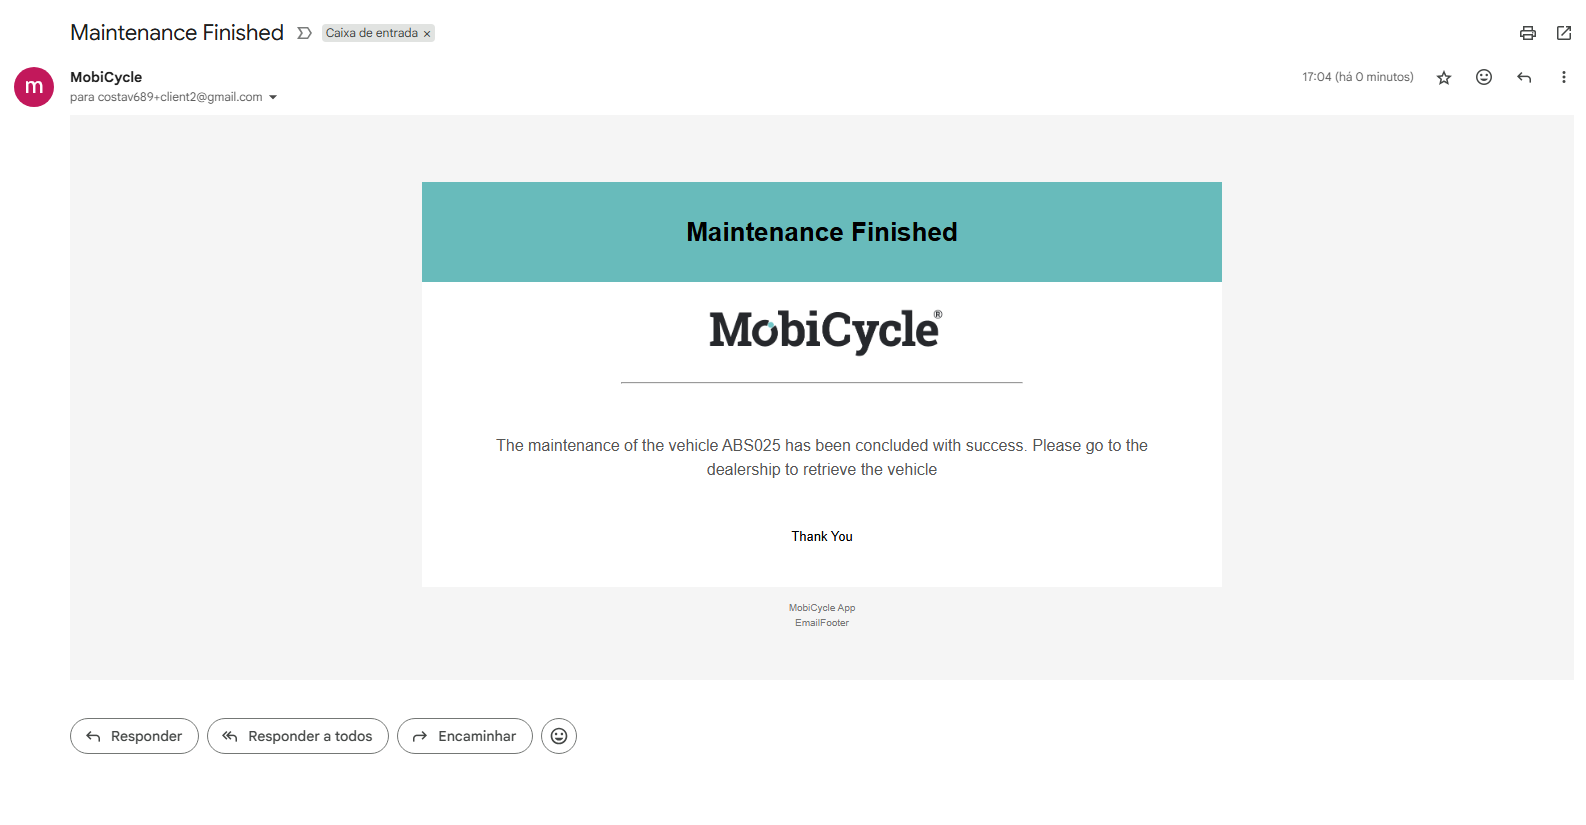
\includegraphics[width=\textwidth]{figs/Implementation/client/MaintenanceFinishedNotification}
  \label{fig:MaintenanceFinishedNotification}
\end{figure}


\begin{figure}[htbp]
  \caption{Client home page with no active maintenance.}
  \centering
  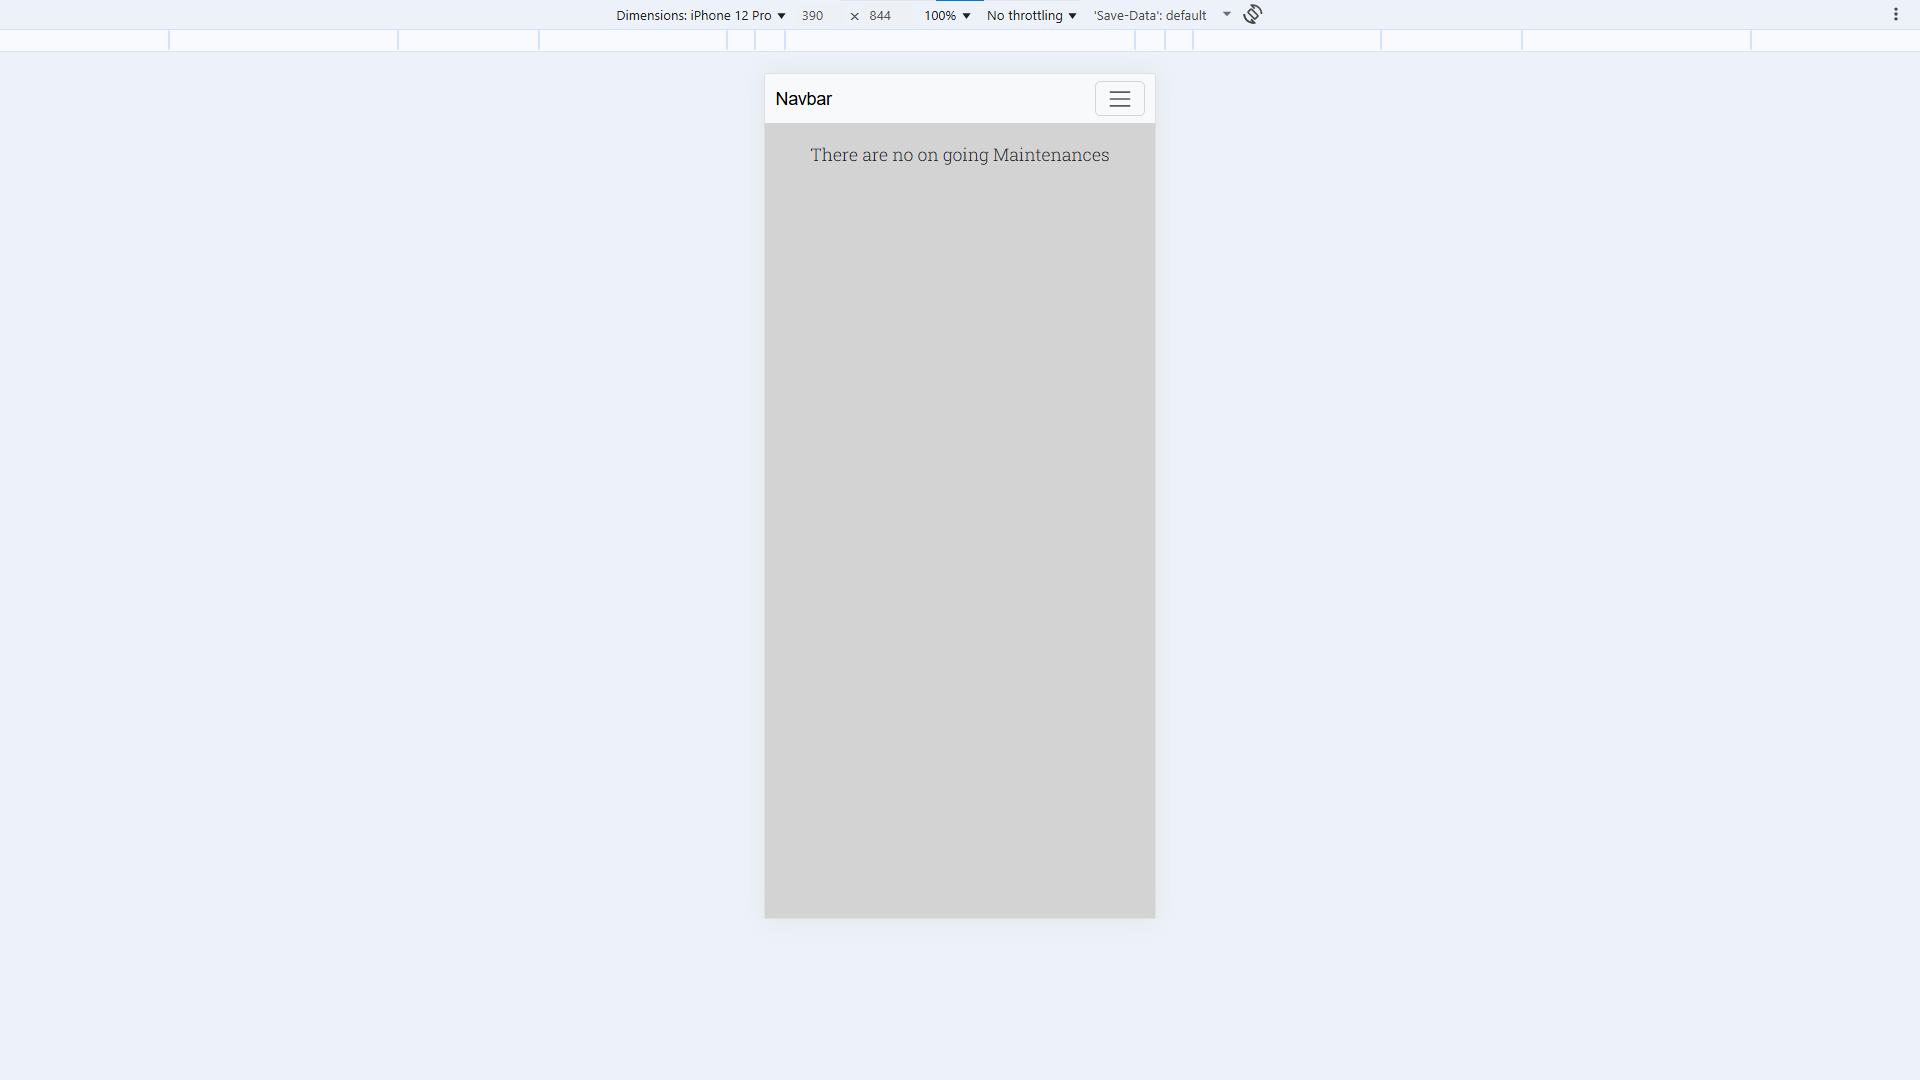
\includegraphics[width=0.30\textwidth]{figs/Implementation/client/MaintenanceNoState}
  \label{fig:MaintenanceNoState}
\end{figure}



\begin{figure}[htbp]
  \caption{Client Home page when he schedules a maintenance with the rececionist.}
  \centering
  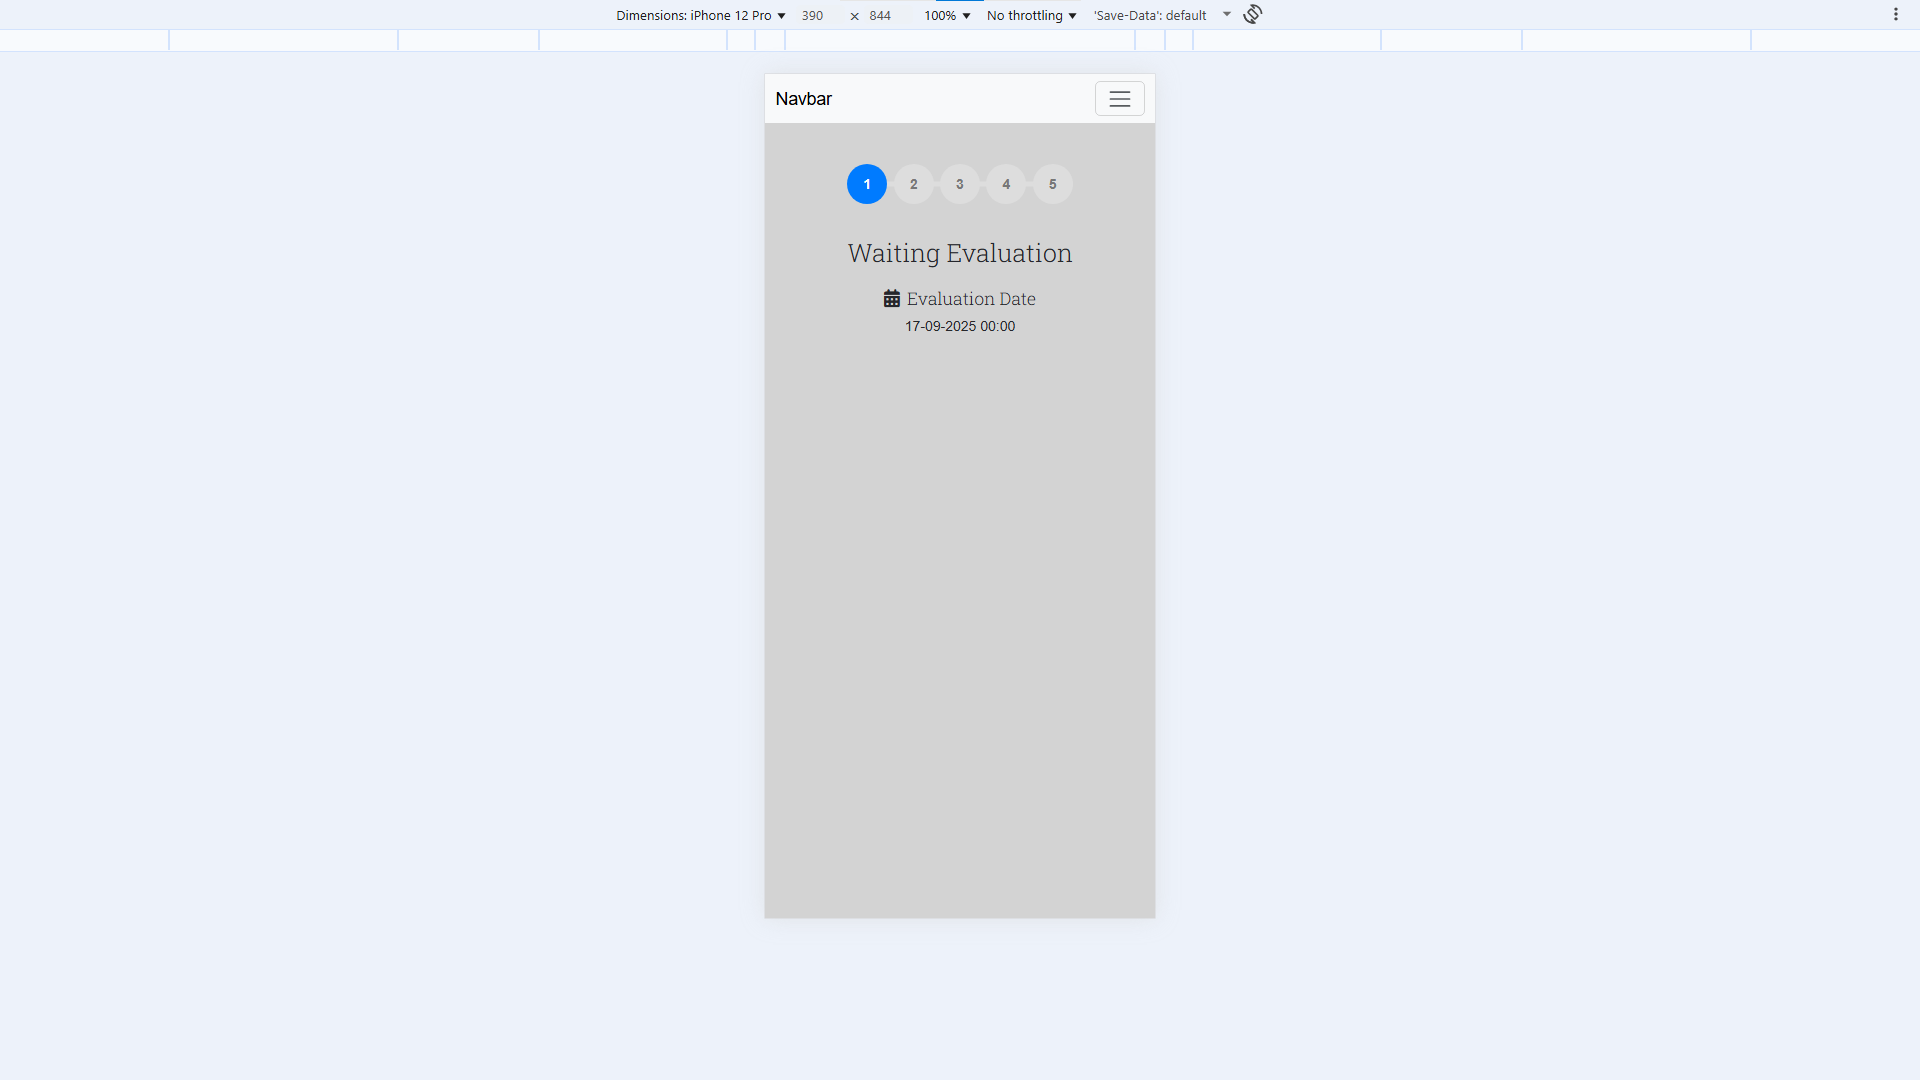
\includegraphics[width=0.30\textwidth]{figs/Implementation/client/MaintenanceState1}
  \label{fig:MaintenanceState1}
\end{figure}




\begin{figure}[htbp]
  \caption{Client Home page when the maintenance is approved.}
  \centering
  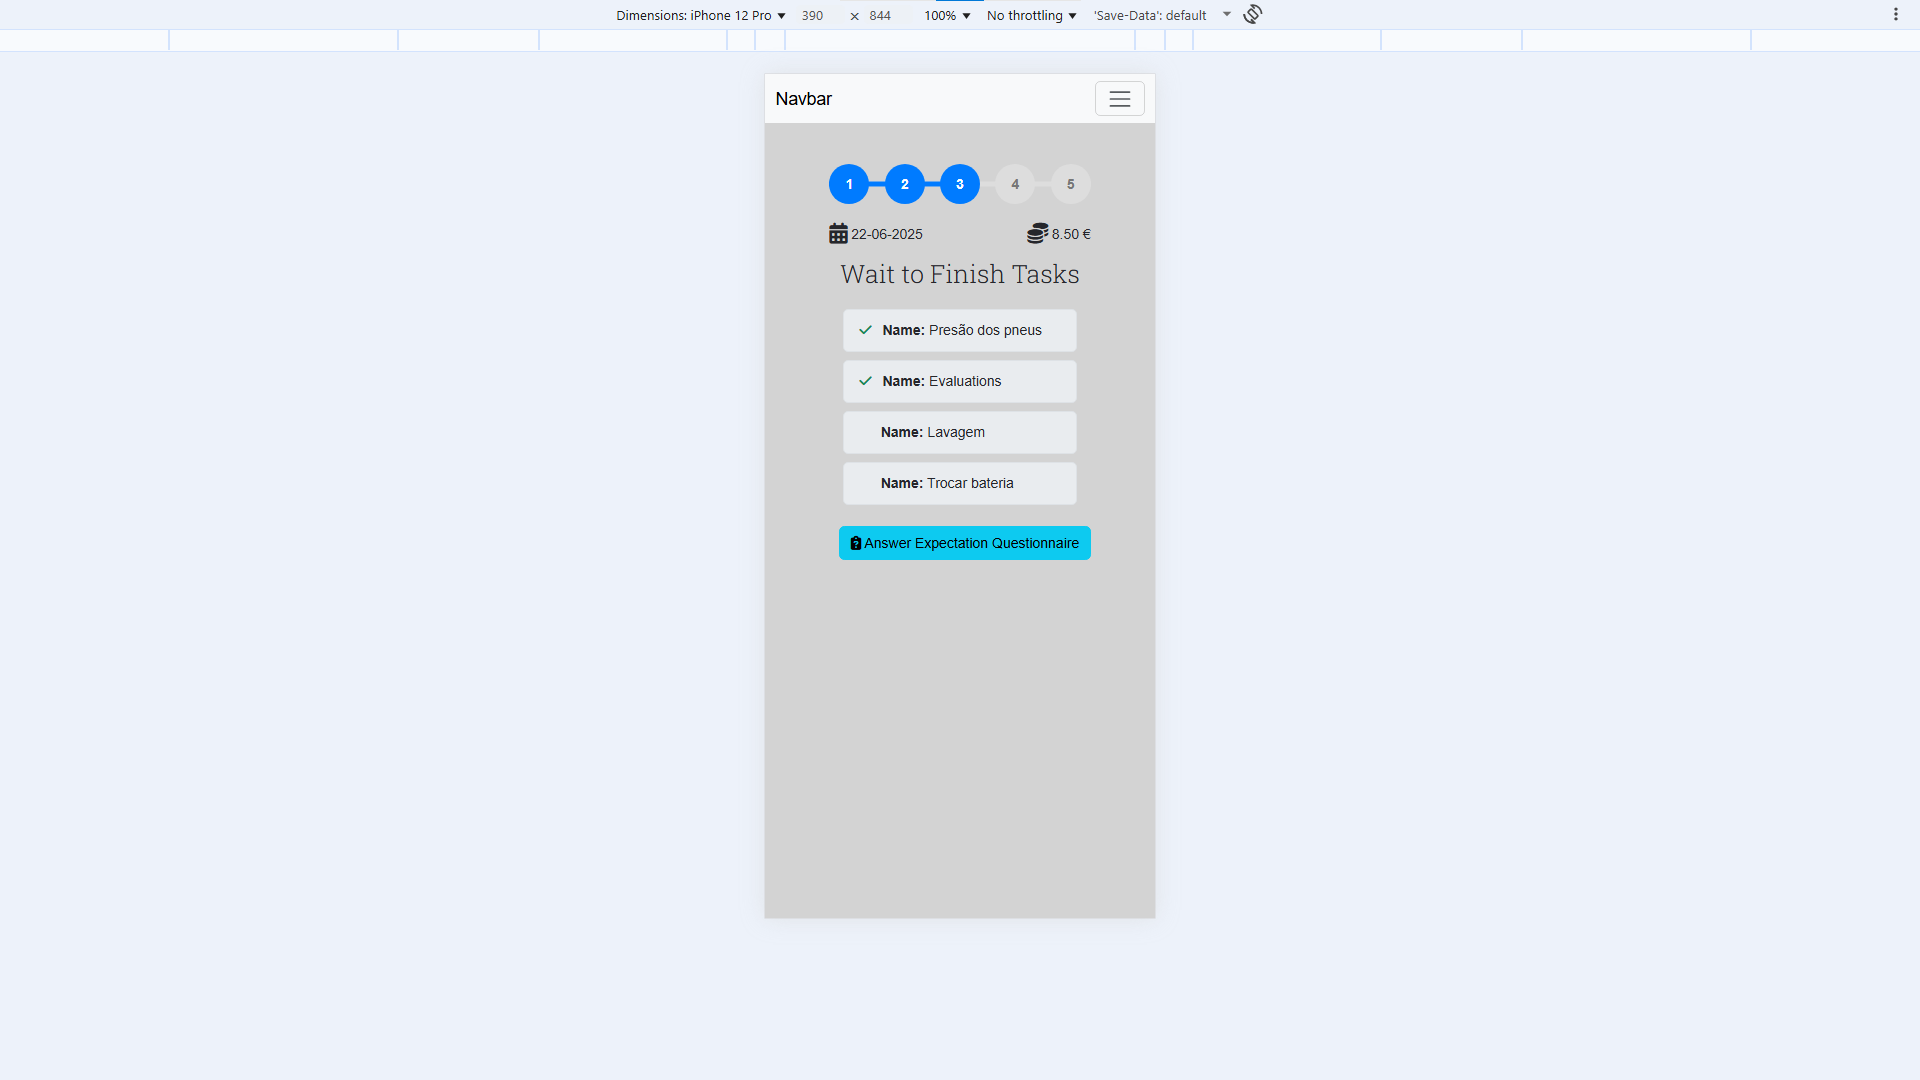
\includegraphics[width=0.30\textwidth]{figs/Implementation/client/MaintenanceState3}
  \label{fig:MaintenanceState3}
\end{figure}


\begin{figure}[htbp]
  \caption{Client Home page when the maintenance tasks are completed and the client can go take the vehicle.}
  \centering
  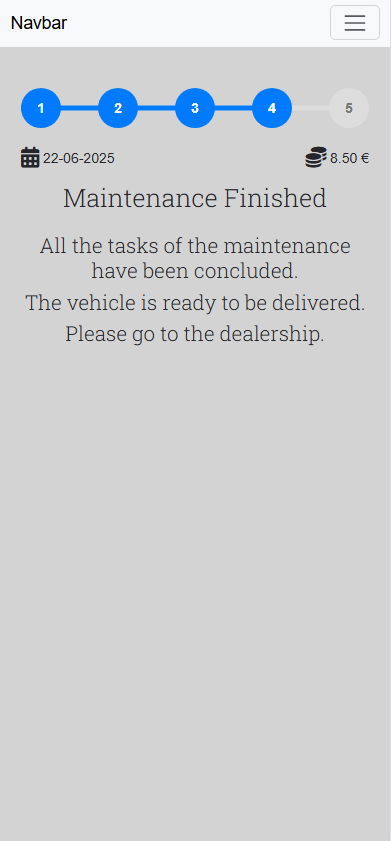
\includegraphics[width=0.30\textwidth]{figs/Implementation/client/MaintenanceState4}
  \label{fig:MaintenanceState4}
\end{figure}


\begin{figure}[htbp]
  \caption{Client Expectation Questionaire refering the questions and introduction in ~\cite{master_servqual_model}.}
  \centering
  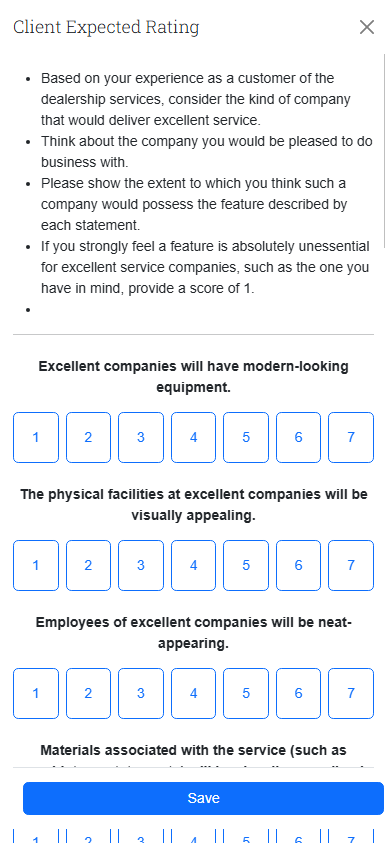
\includegraphics[width=0.30\textwidth]{figs/Implementation/client/ExpectationQuestionare}
  \label{fig:ExpectationQuestionare}
\end{figure}


\begin{figure}[htbp]
  \caption{Client Perception Questionaire refering the questions and introduction in ~\cite{master_servqual_model}.}
  \centering
  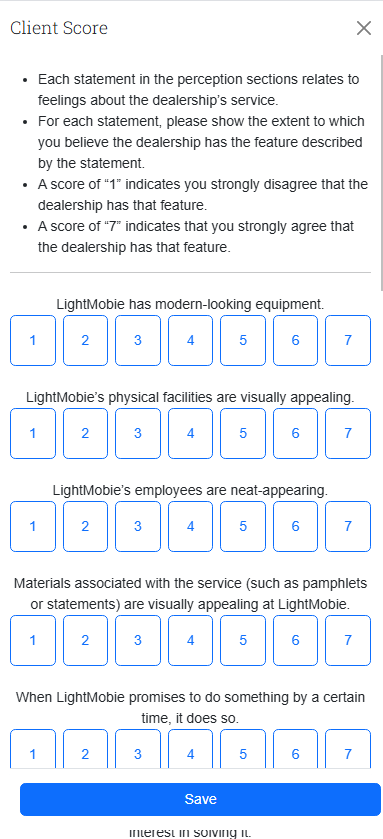
\includegraphics[width=0.30\textwidth]{figs/Implementation/client/PerceptionQuestionare}
  \label{fig:PerceptionQuestionare}
\end{figure}


\begin{figure}[htbp]
  \caption{Details of a maintenance example the tab of information.}
  \centering
  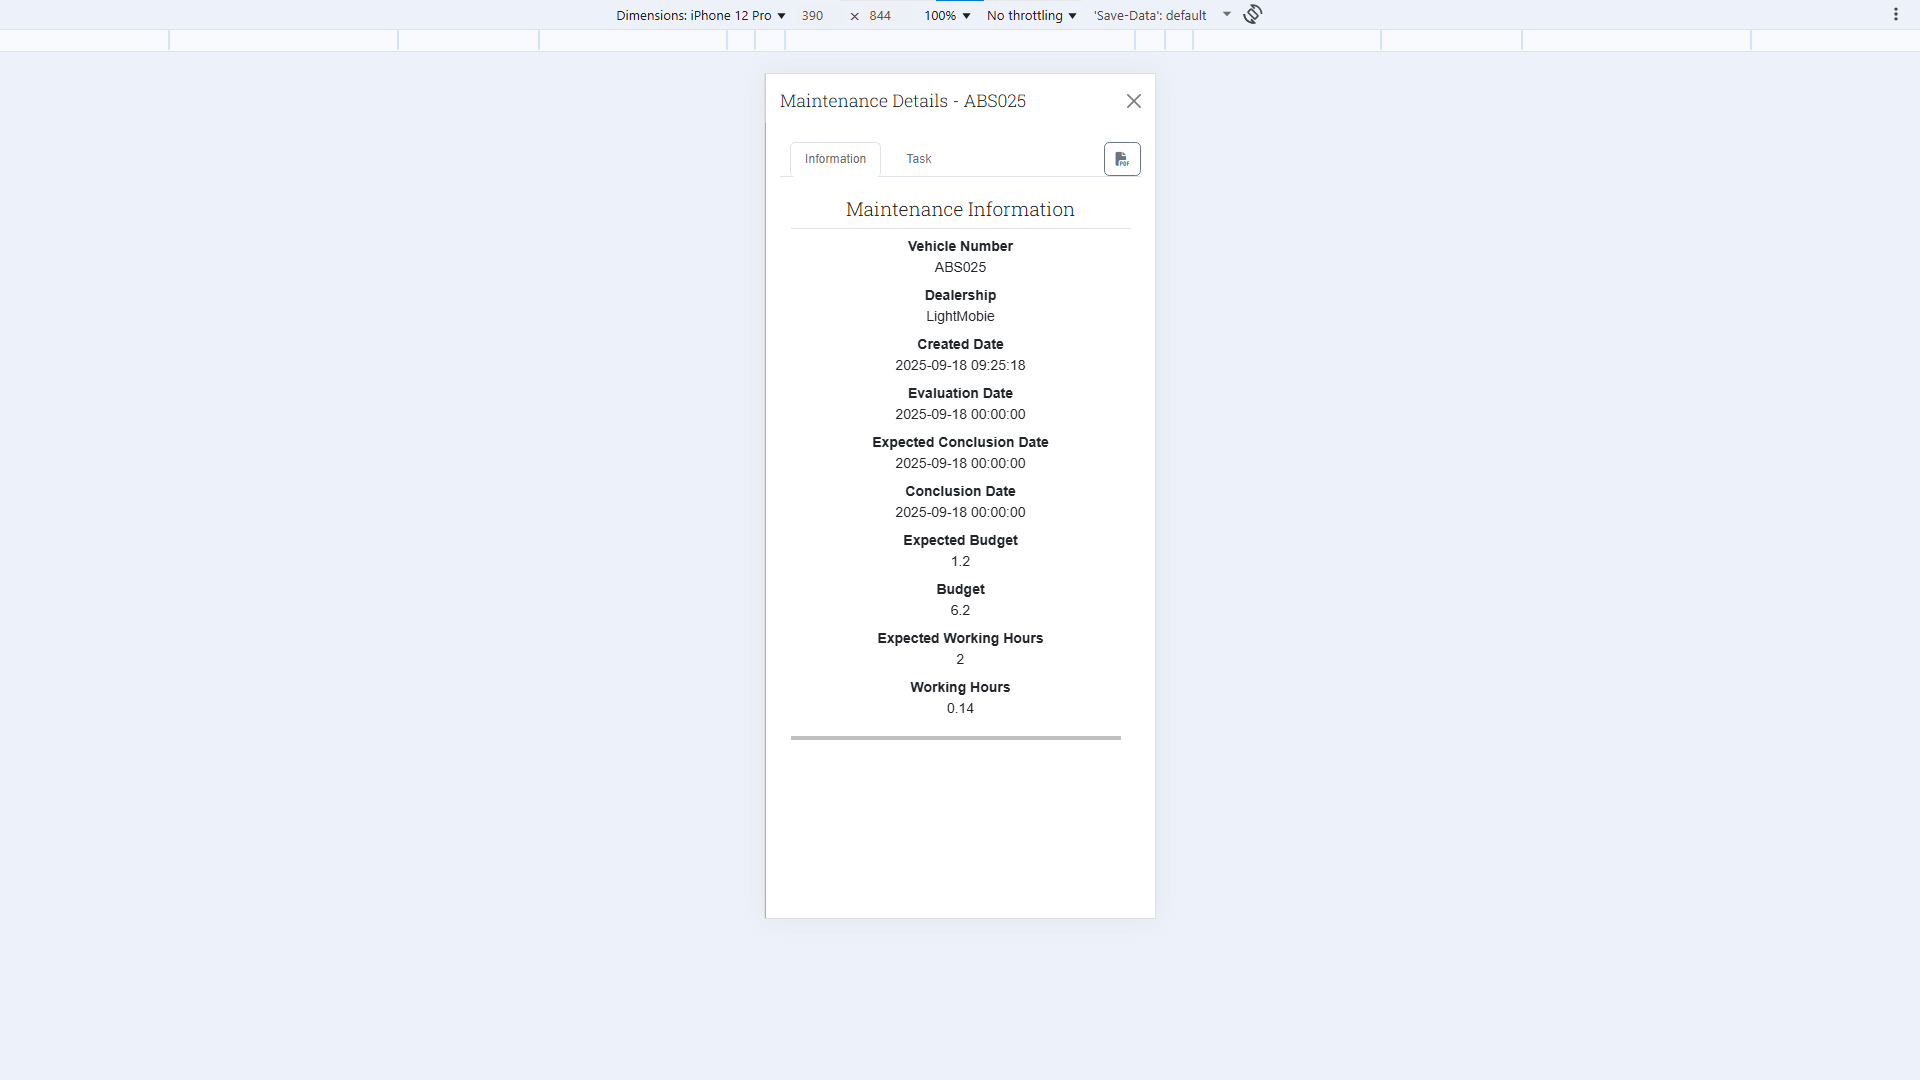
\includegraphics[width=0.30\textwidth]{figs/Implementation/client/MaintenanceDetailsInfo}
  \label{fig:MaintenanceDetailsInfo}
\end{figure}


\begin{figure}[htbp]
  \caption{Details of a maintenance example the list of task.}
  \centering
  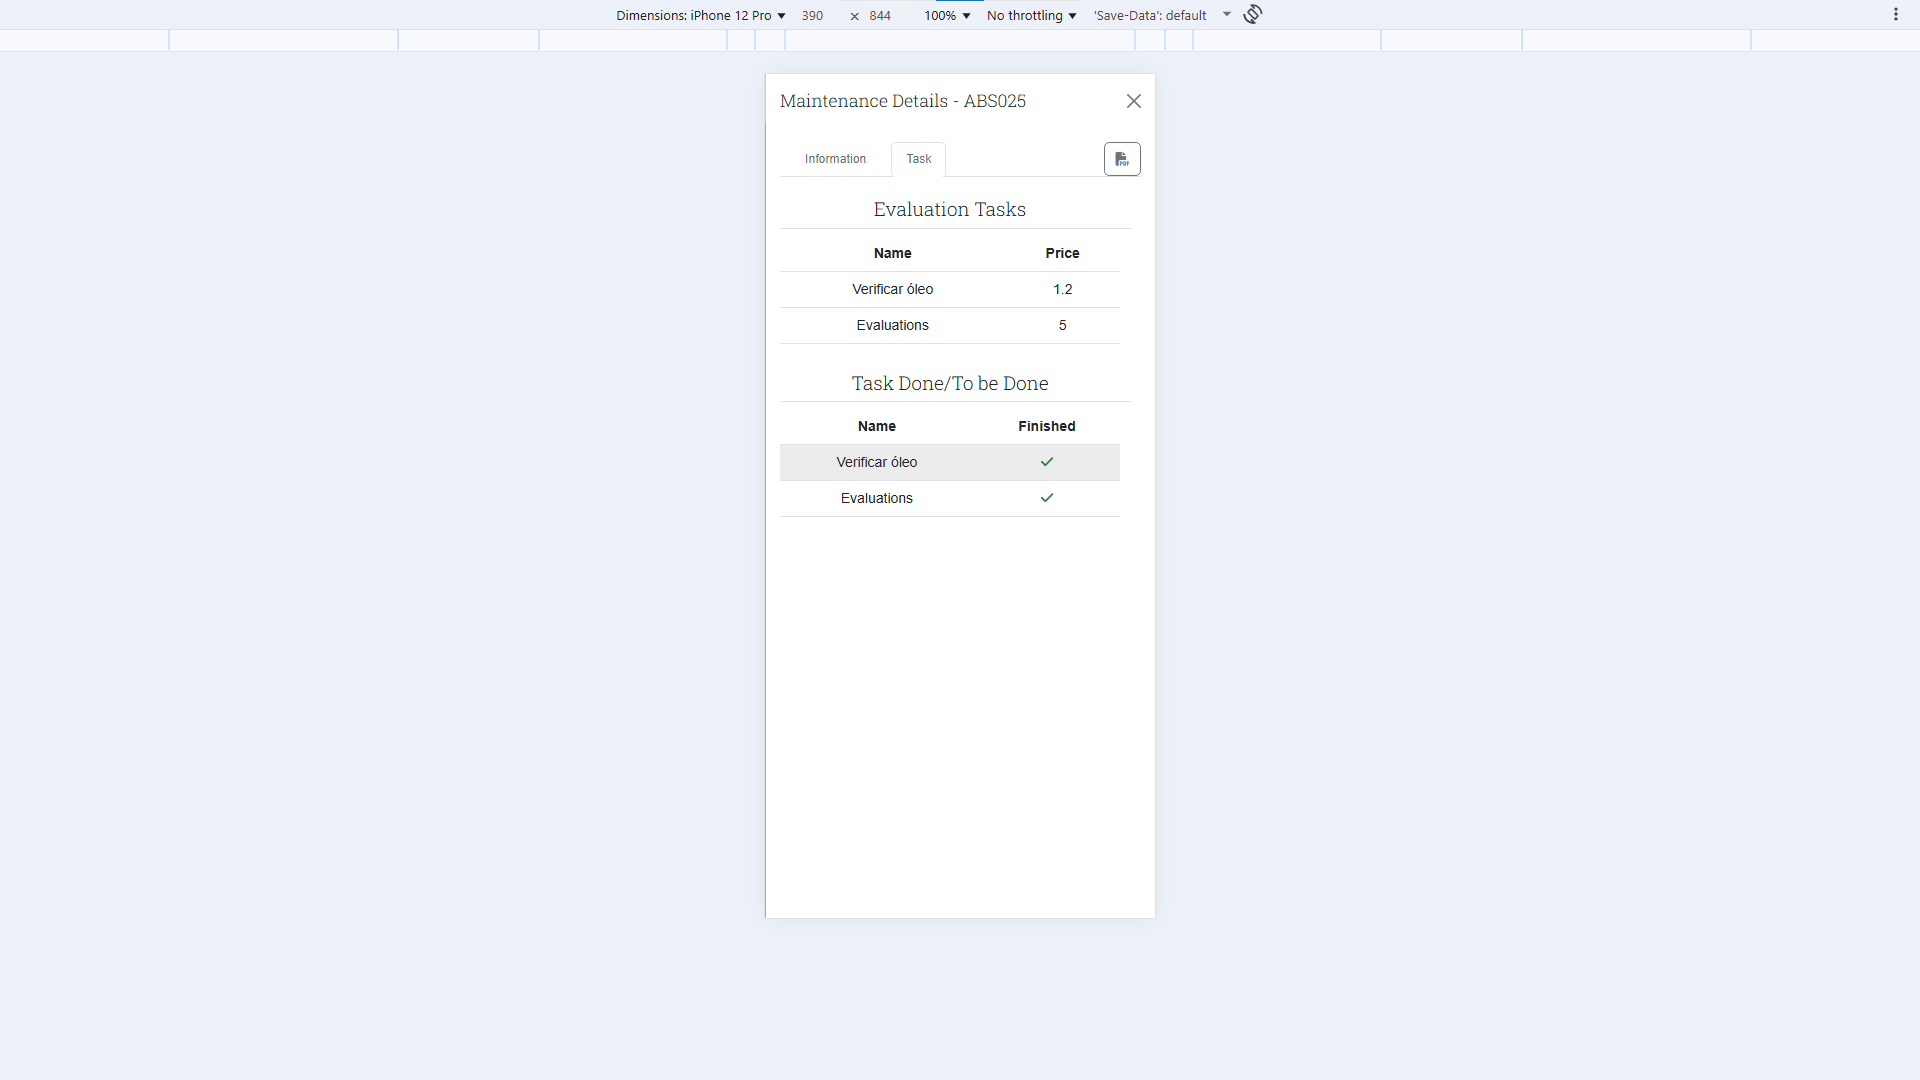
\includegraphics[width=0.30\textwidth]{figs/Implementation/client/MaintenanceDetailsTasks}
  \label{fig:MaintenanceDetailsTasks}
\end{figure}




\begin{figure}[htbp]
  \caption{Parts type details.}
  \centering
  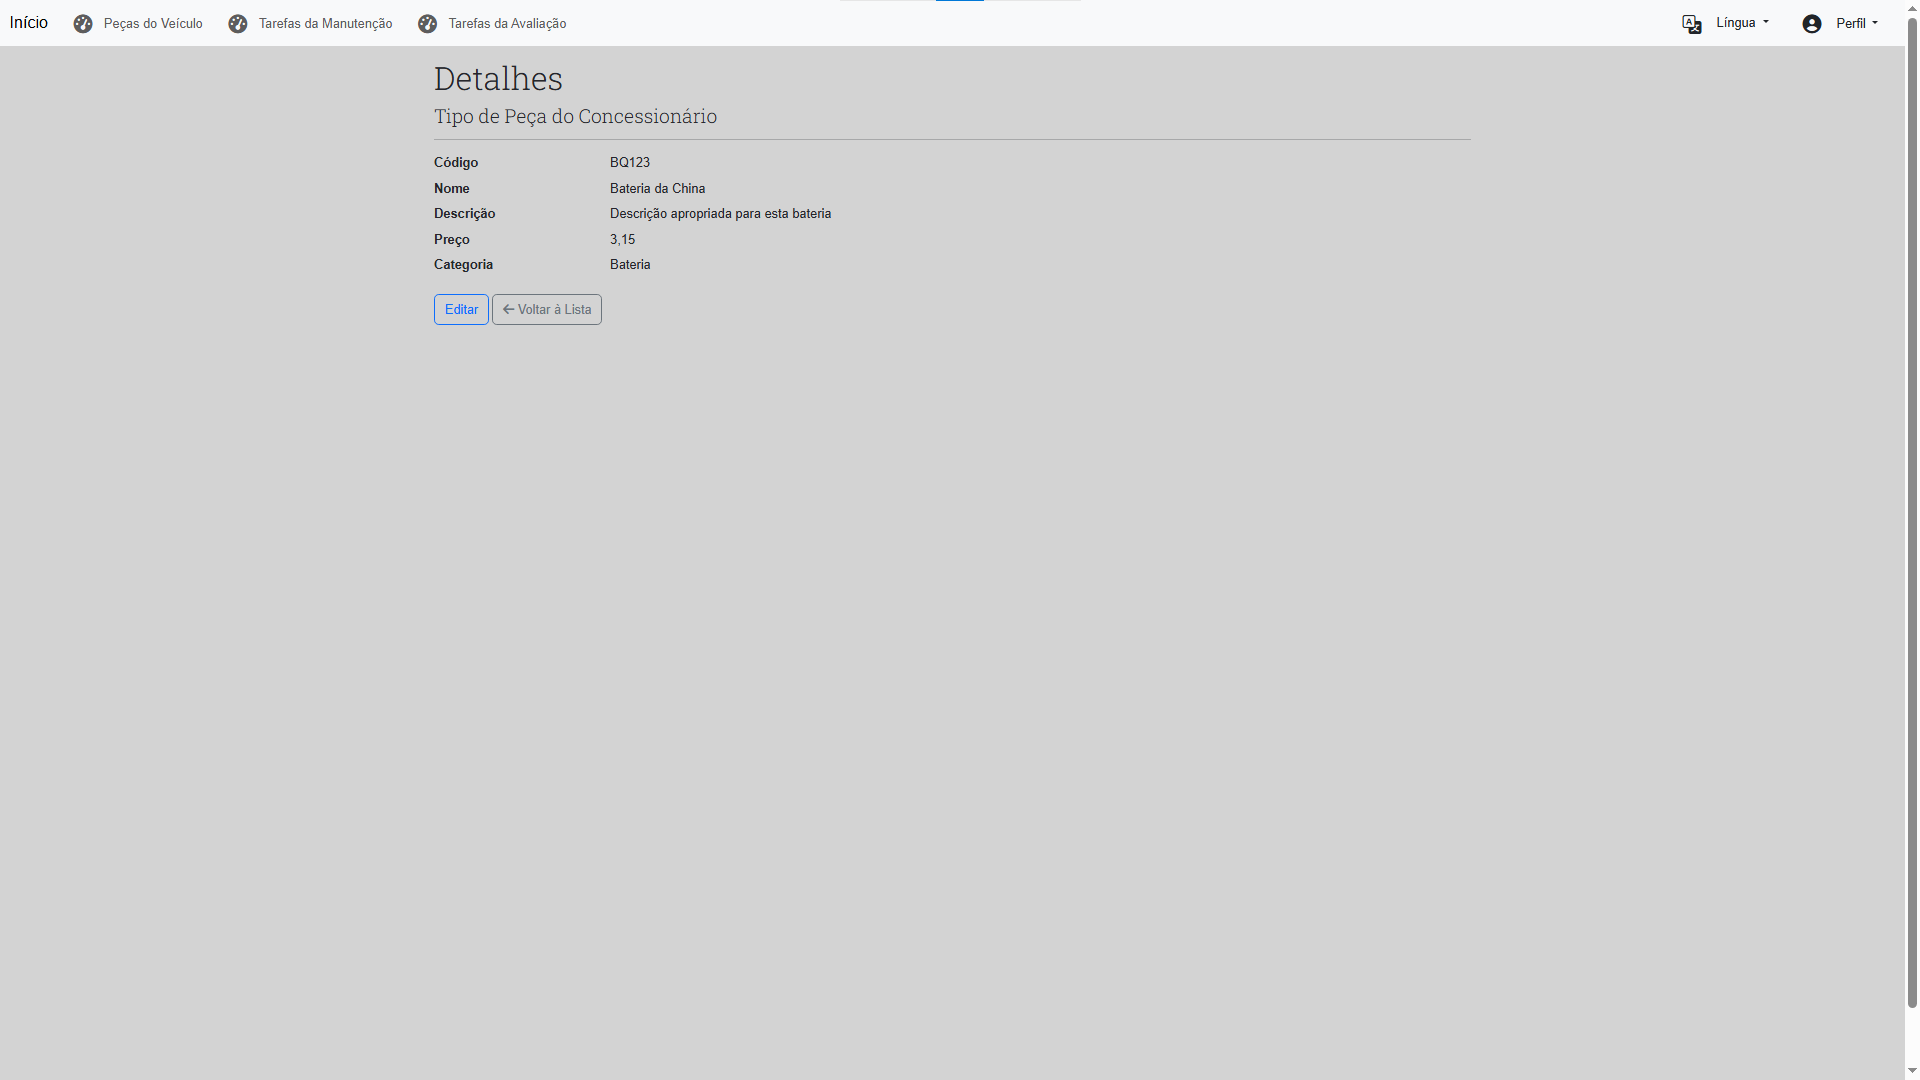
\includegraphics[width=\textwidth]{figs/Implementation/dealershipAdmin/partsDetails}
  \label{fig:partsDetails}
\end{figure}

\begin{figure}[htbp]
  \caption{Parts type edit.}
  \centering
  \includegraphics[width=\textwidth]{figs/Implementation/dealershipAdmin/partsEdit}
  \label{fig:partsEdit}
\end{figure}

\begin{figure}[htbp]
  \caption{Parts type delete.}
  \centering
  \includegraphics[width=\textwidth]{figs/Implementation/dealershipAdmin/partsDelete}
  \label{fig:partsDelete}
\end{figure}


\begin{figure}[htbp]
  \caption{Parts type create.}
  \centering
  \includegraphics[width=\textwidth]{figs/Implementation/dealershipAdmin/partsCreate}
  \label{fig:partsCreate}
\end{figure}



\begin{figure}[htbp]
  \caption{Task type list index.}
  \centering
  \includegraphics[width=\textwidth]{figs/Implementation/dealershipAdmin/taskIndex}
  \label{fig:taskIndex}
\end{figure}

\clearpage

\begin{figure}[htbp]
  \caption{Eval task list index.}
  \centering
  \includegraphics[width=\textwidth]{figs/Implementation/dealershipAdmin/evalIndex}
  \label{fig:evalIndex}
\end{figure}
 
\begin{figure}[htbp] 
  \caption{Eval task edit.}
  \centering
  \includegraphics[width=\textwidth]{figs/Implementation/dealershipAdmin/evalEdit}
  \label{fig:evalEdit} 
\end{figure}


\begin{figure}[htbp]
  \caption{Task type edit.}
  \centering
  \includegraphics[width=\textwidth]{figs/Implementation/dealershipAdmin/taskEdit}
  \label{fig:taskEdit}
\end{figure}


\begin{figure}[htbp]
  \caption{Task type details.}
  \centering
  \includegraphics[width=\textwidth]{figs/Implementation/dealershipAdmin/taskDetails}
  \label{fig:taskDetails}
\end{figure}

 
\begin{figure}[htbp]
  \caption{Task type delete.}
  \centering
  \includegraphics[width=\textwidth]{figs/Implementation/dealershipAdmin/taskDelete}
  \label{fig:taskDelete}
\end{figure}

\begin{figure}[htbp]
  \caption{Task type create.}
  \centering
  \includegraphics[width=\textwidth]{figs/Implementation/dealershipAdmin/taskCreate}
  \label{fig:taskCreate}
\end{figure}


\begin{figure}[htbp]
  \caption{Eval task create.}
  \centering
  \includegraphics[width=\textwidth]{figs/Implementation/dealershipAdmin/evalCreate}
  \label{fig:evalCreate}
\end{figure}

\begin{figure}[htbp]
  \caption{Eval task delete.}
  \centering
  \includegraphics[width=\textwidth]{figs/Implementation/dealershipAdmin/evalDelete}
  \label{fig:evalDelete}
\end{figure}

\begin{figure}[htbp]
  \caption{Eval task details.}
  \centering
  \includegraphics[width=\textwidth]{figs/Implementation/dealershipAdmin/evalDetails}
  \label{fig:evalDetails}
\end{figure}

\foreach \p in {1,...,11}{%  <-- change 5 to the total number of pages
\begin{figure}[p]
  \caption{User tests tasks — page \p}
  \centering
  \includegraphics[page=\p,width=\textwidth]{figs/chapter5/UserTestsTasksEnglish}
  \label{fig:UserTestsTasks-\p}
\end{figure}
}

\foreach \p in {1,...,6}{%  <-- change 5 to the total number of pages
\begin{figure}[p]
  \caption{Aplication questionaire— page \p}
  \centering
  \includegraphics[page=\p,width=\textwidth]{figs/chapter5/AplicationQuestionaire}
  \label{fig:AplicationQuestionaire-\p}
\end{figure}  
}






\end{document}
